
\allowdisplaybreaks % makes it so align envs can span between multiple pages

%\setcounter{chapter}{31}
\chapter{Generative Models}
\label{chapter:generative_models}
\index{Generative models}

\section{Introduction}
Generative models perform (or describe) the synthesis of data. Recall the image classifier from \chap{\ref{chapter:intro_to_learning}}, shown again below (\fig{\ref{fig:gen_models_image_classification}}):

\begin{figure}[h]
    \centerline{
    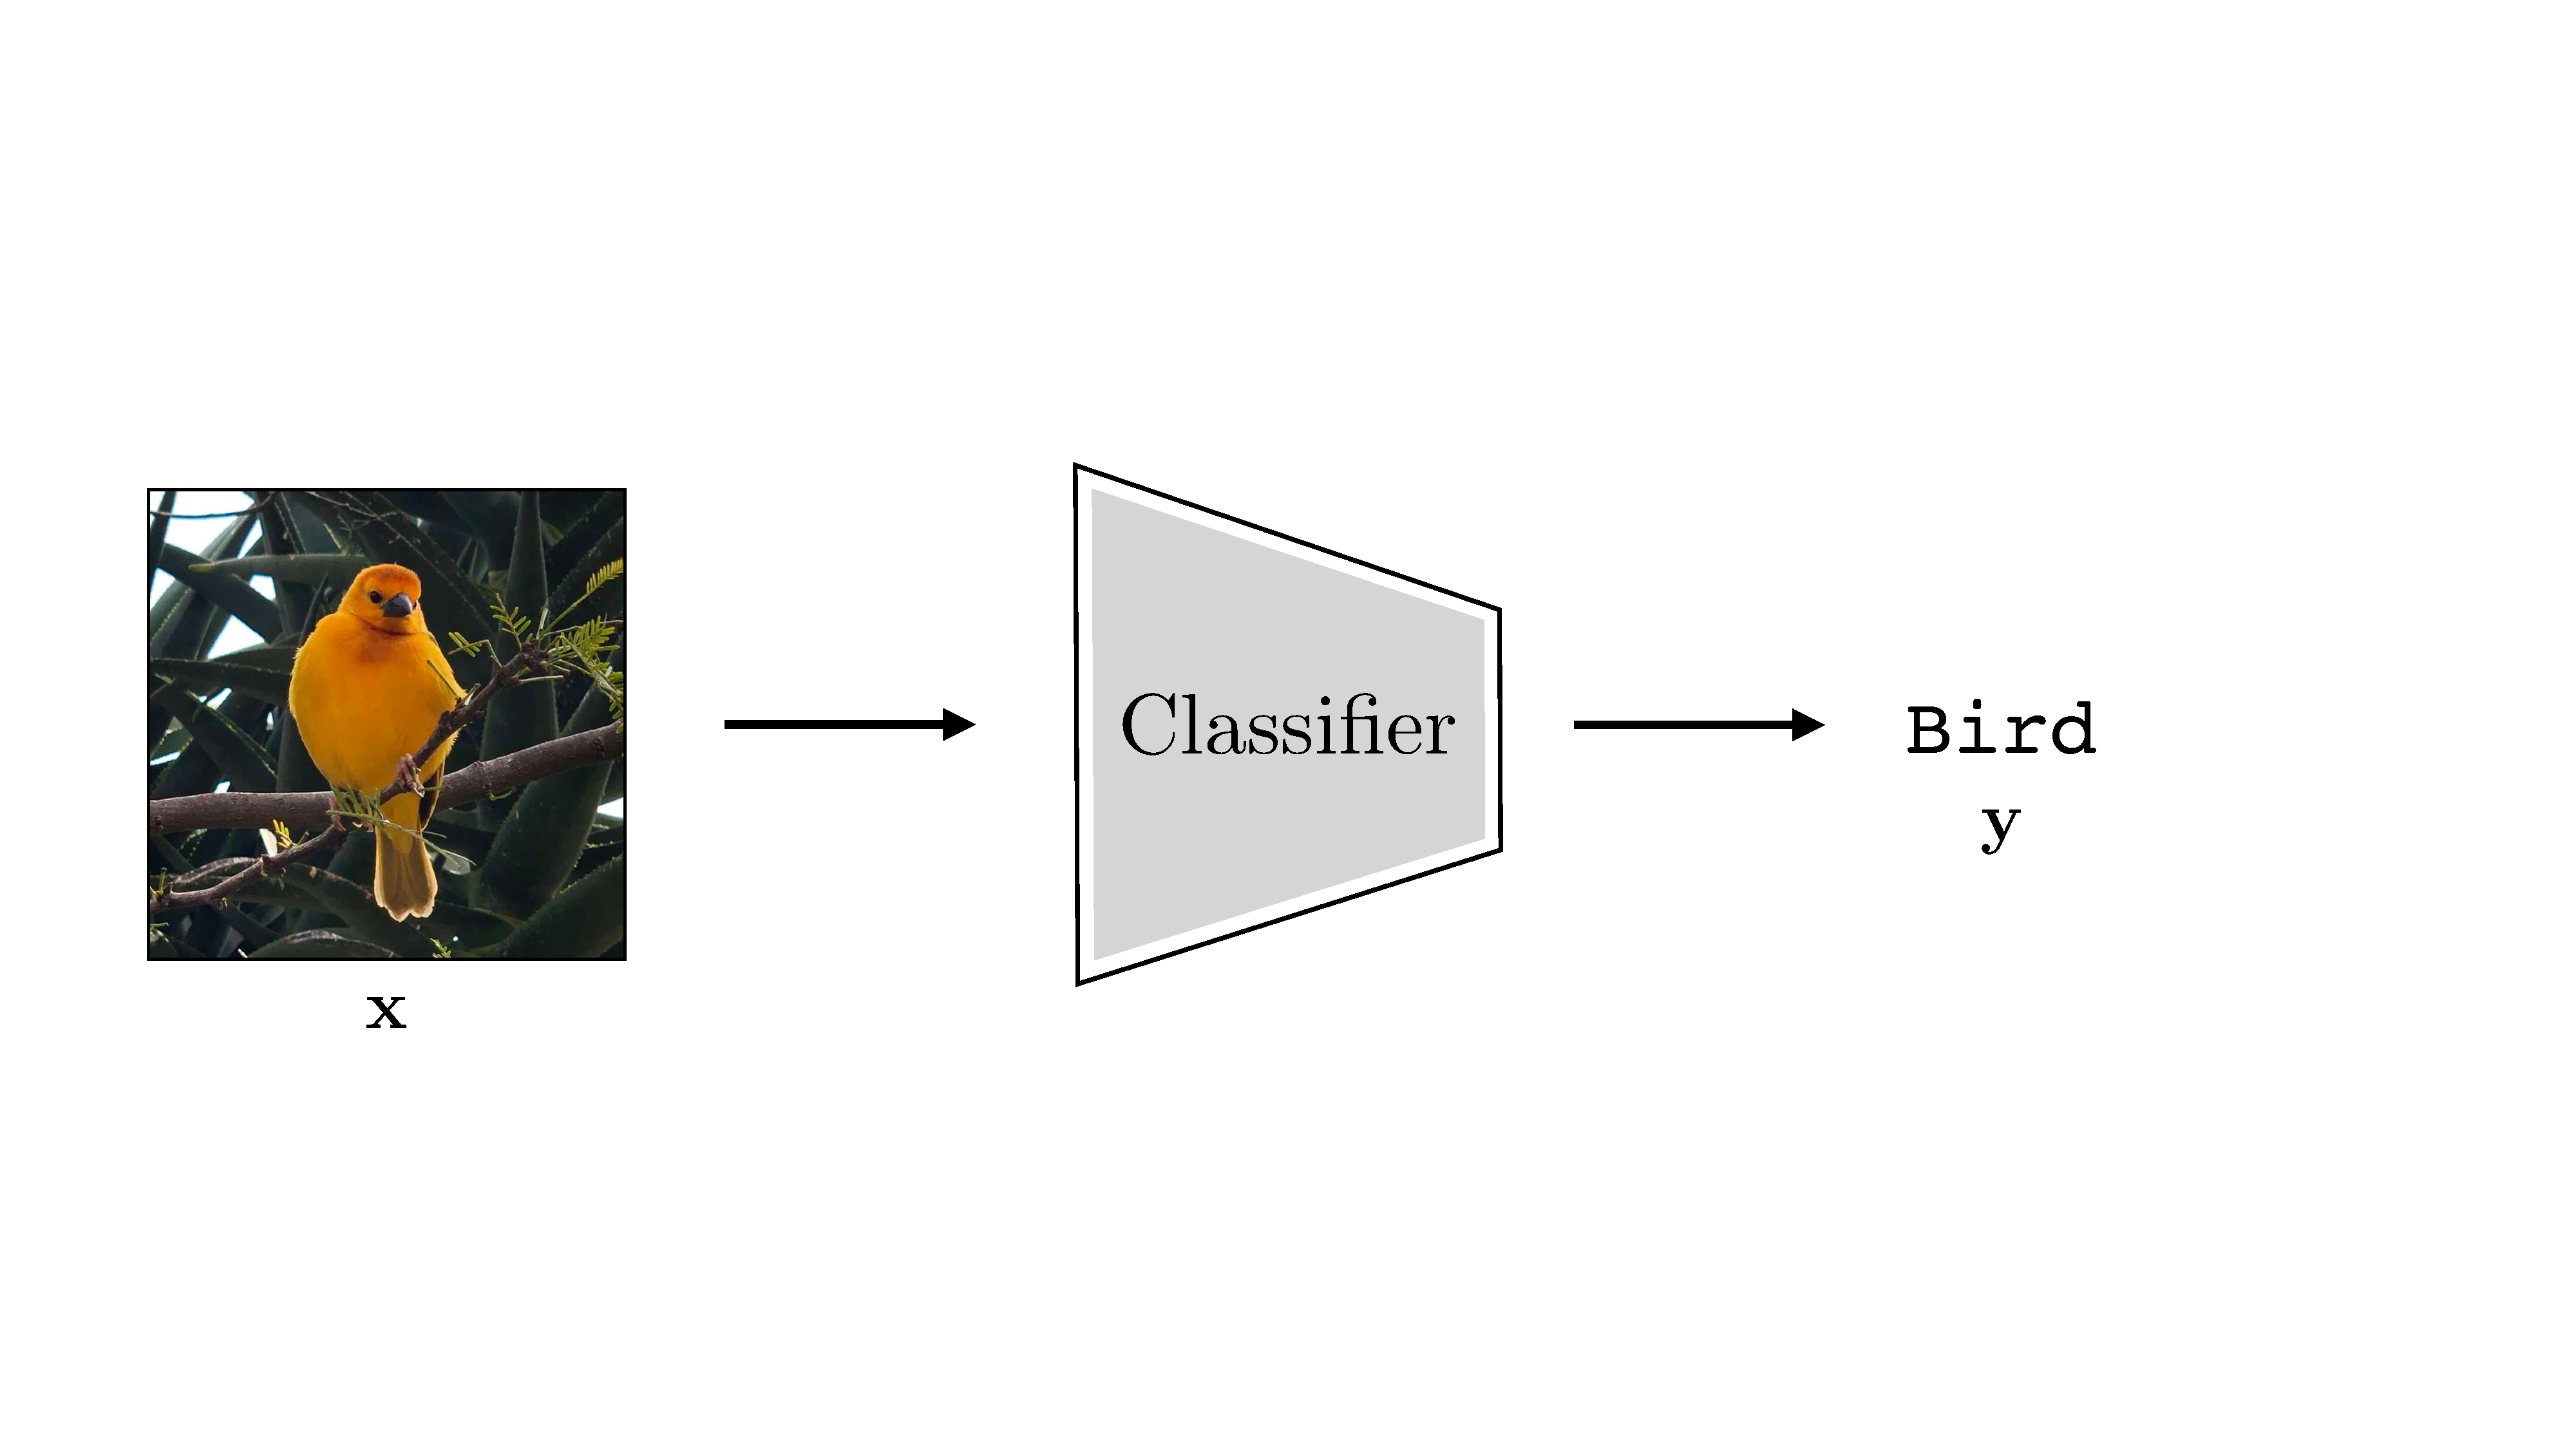
\includegraphics[width=0.7\linewidth]{./figures/generative_models/image_classification_bird.pdf}
    }
    \caption{A classifier maps images to labels.}
    \label{fig:gen_models_image_classification}
\end{figure}

A generative model does the opposite (\fig{\ref{fig:gen_models_image_generation}}):

\begin{figure}[h]
    \centerline{
    \hspace*{0.05\linewidth}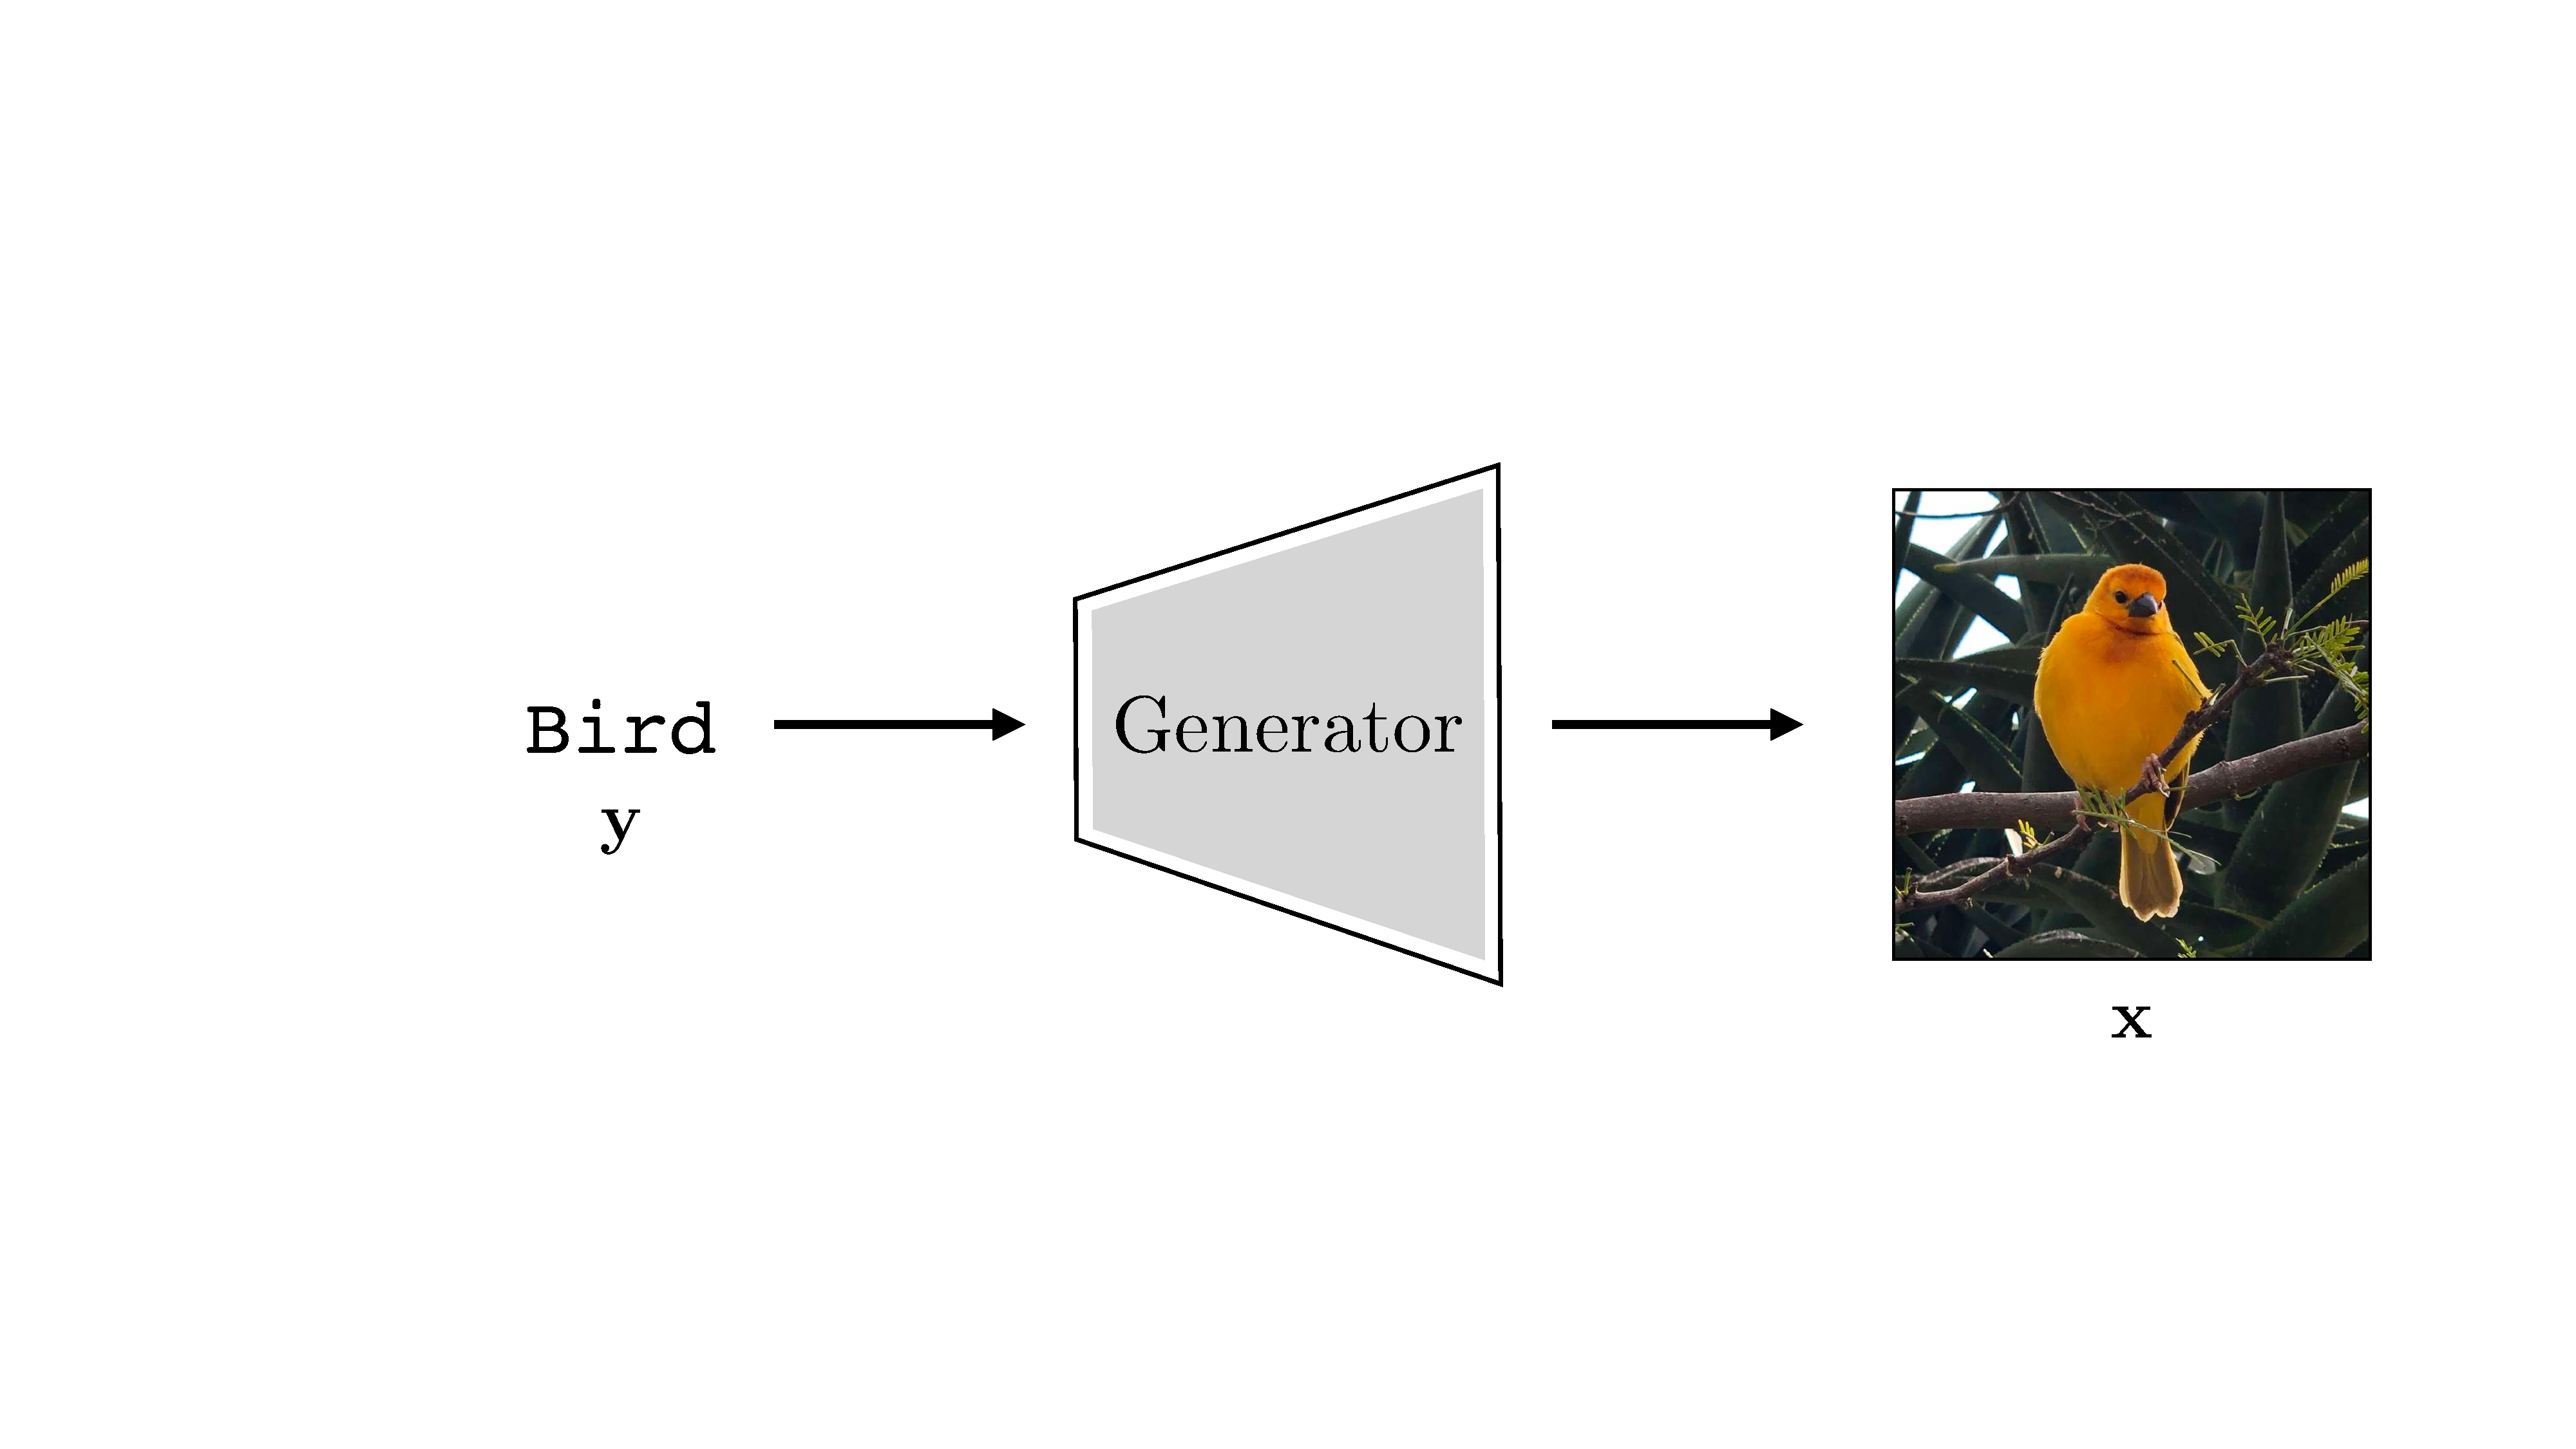
\includegraphics[width=0.7\linewidth]{./figures/generative_models/image_generation_bird.pdf}
    }
    \caption{A generator maps labels (or other descriptions) to images.}
    \label{fig:gen_models_image_generation}
\end{figure}

Whereas an image classifier is a function $f: \mathcal{X} \rightarrow \mathcal{Y}$, a generative model is a function in the opposite direction $g: \mathcal{Y} \rightarrow \mathcal{X}$. Things are a bit different in this direction. The function $f$ is {\bf many-to-one}: there are many images that all should be given the same label ``bird.'' The function $g$, conversely, is {\bf one-to-many}: there are many possible outputs for any given input. Generative models handle this ambiguity by making $g$ a {\bf stochastic function}.\marginnote{Although we describe $\mathbf{y}$ as a label here, generative models can in fact take other kinds of instructions as inputs, such as text descriptions of what we want to generate or hand-drawn sketches that we wish the model to fill in.}[-1.8cm]
%\marginnote{In this chapter, note that if $X$ is a random variable, $\mathbf{x}$ is a realization of this variable, and $\mathbf{X}$ is the domain of that variable. The same applies to $Y$, $Z$, and so on.}[-1.8cm]%\marginnote{$\mathbf{y} \in \mathcal{Y}$ is a class label in this example. We write it in bold since labels are usually represented as vectors, e.g., one-hot codes.}[-1cm]

One way to make a function stochastic is to make it a deterministic function of a stochastic input, and this is how most of the generative models in this chapter will work. We define $g$ as a function, called a \index{Generator}\textbf{generator}, that takes a randomized vector $\mathbf{z}$ as input along with the label/description $\mathbf{y}$, and produces an image $\mathbf{x}$ as output, that is, $g: \mathcal{Z} \times \mathcal{Y} \rightarrow \mathcal{X}$. Then this function can output a different image $\mathbf{x}$ for each different setting of $\mathbf{z}$. The generative process is as follows. First sample $\mathbf{z}$ from a prior $p(Z)$, then deterministically generate an image based on $\mathbf{z}$ and $\mathbf{y}$:
\begin{align}
    \mathbf{z} \sim p(Z)\\
    \mathbf{x} = g(\mathbf{z},\mathbf{y})
\end{align}
\marginnote{Graphical model for generating $X \given Y, Z$:\\[6pt]
   \centerline{
   \includegraphics[width=0.15\linewidth]{./figures/generative_models/graphical_model_y_z_to_x_white.eps}}
}[-1.8cm]
This procedure is shown in \fig{\ref{fig:generative_models:image_generation_with_z}}:
\begin{figure}[h]
    \centerline{
    \hspace*{0.1\linewidth}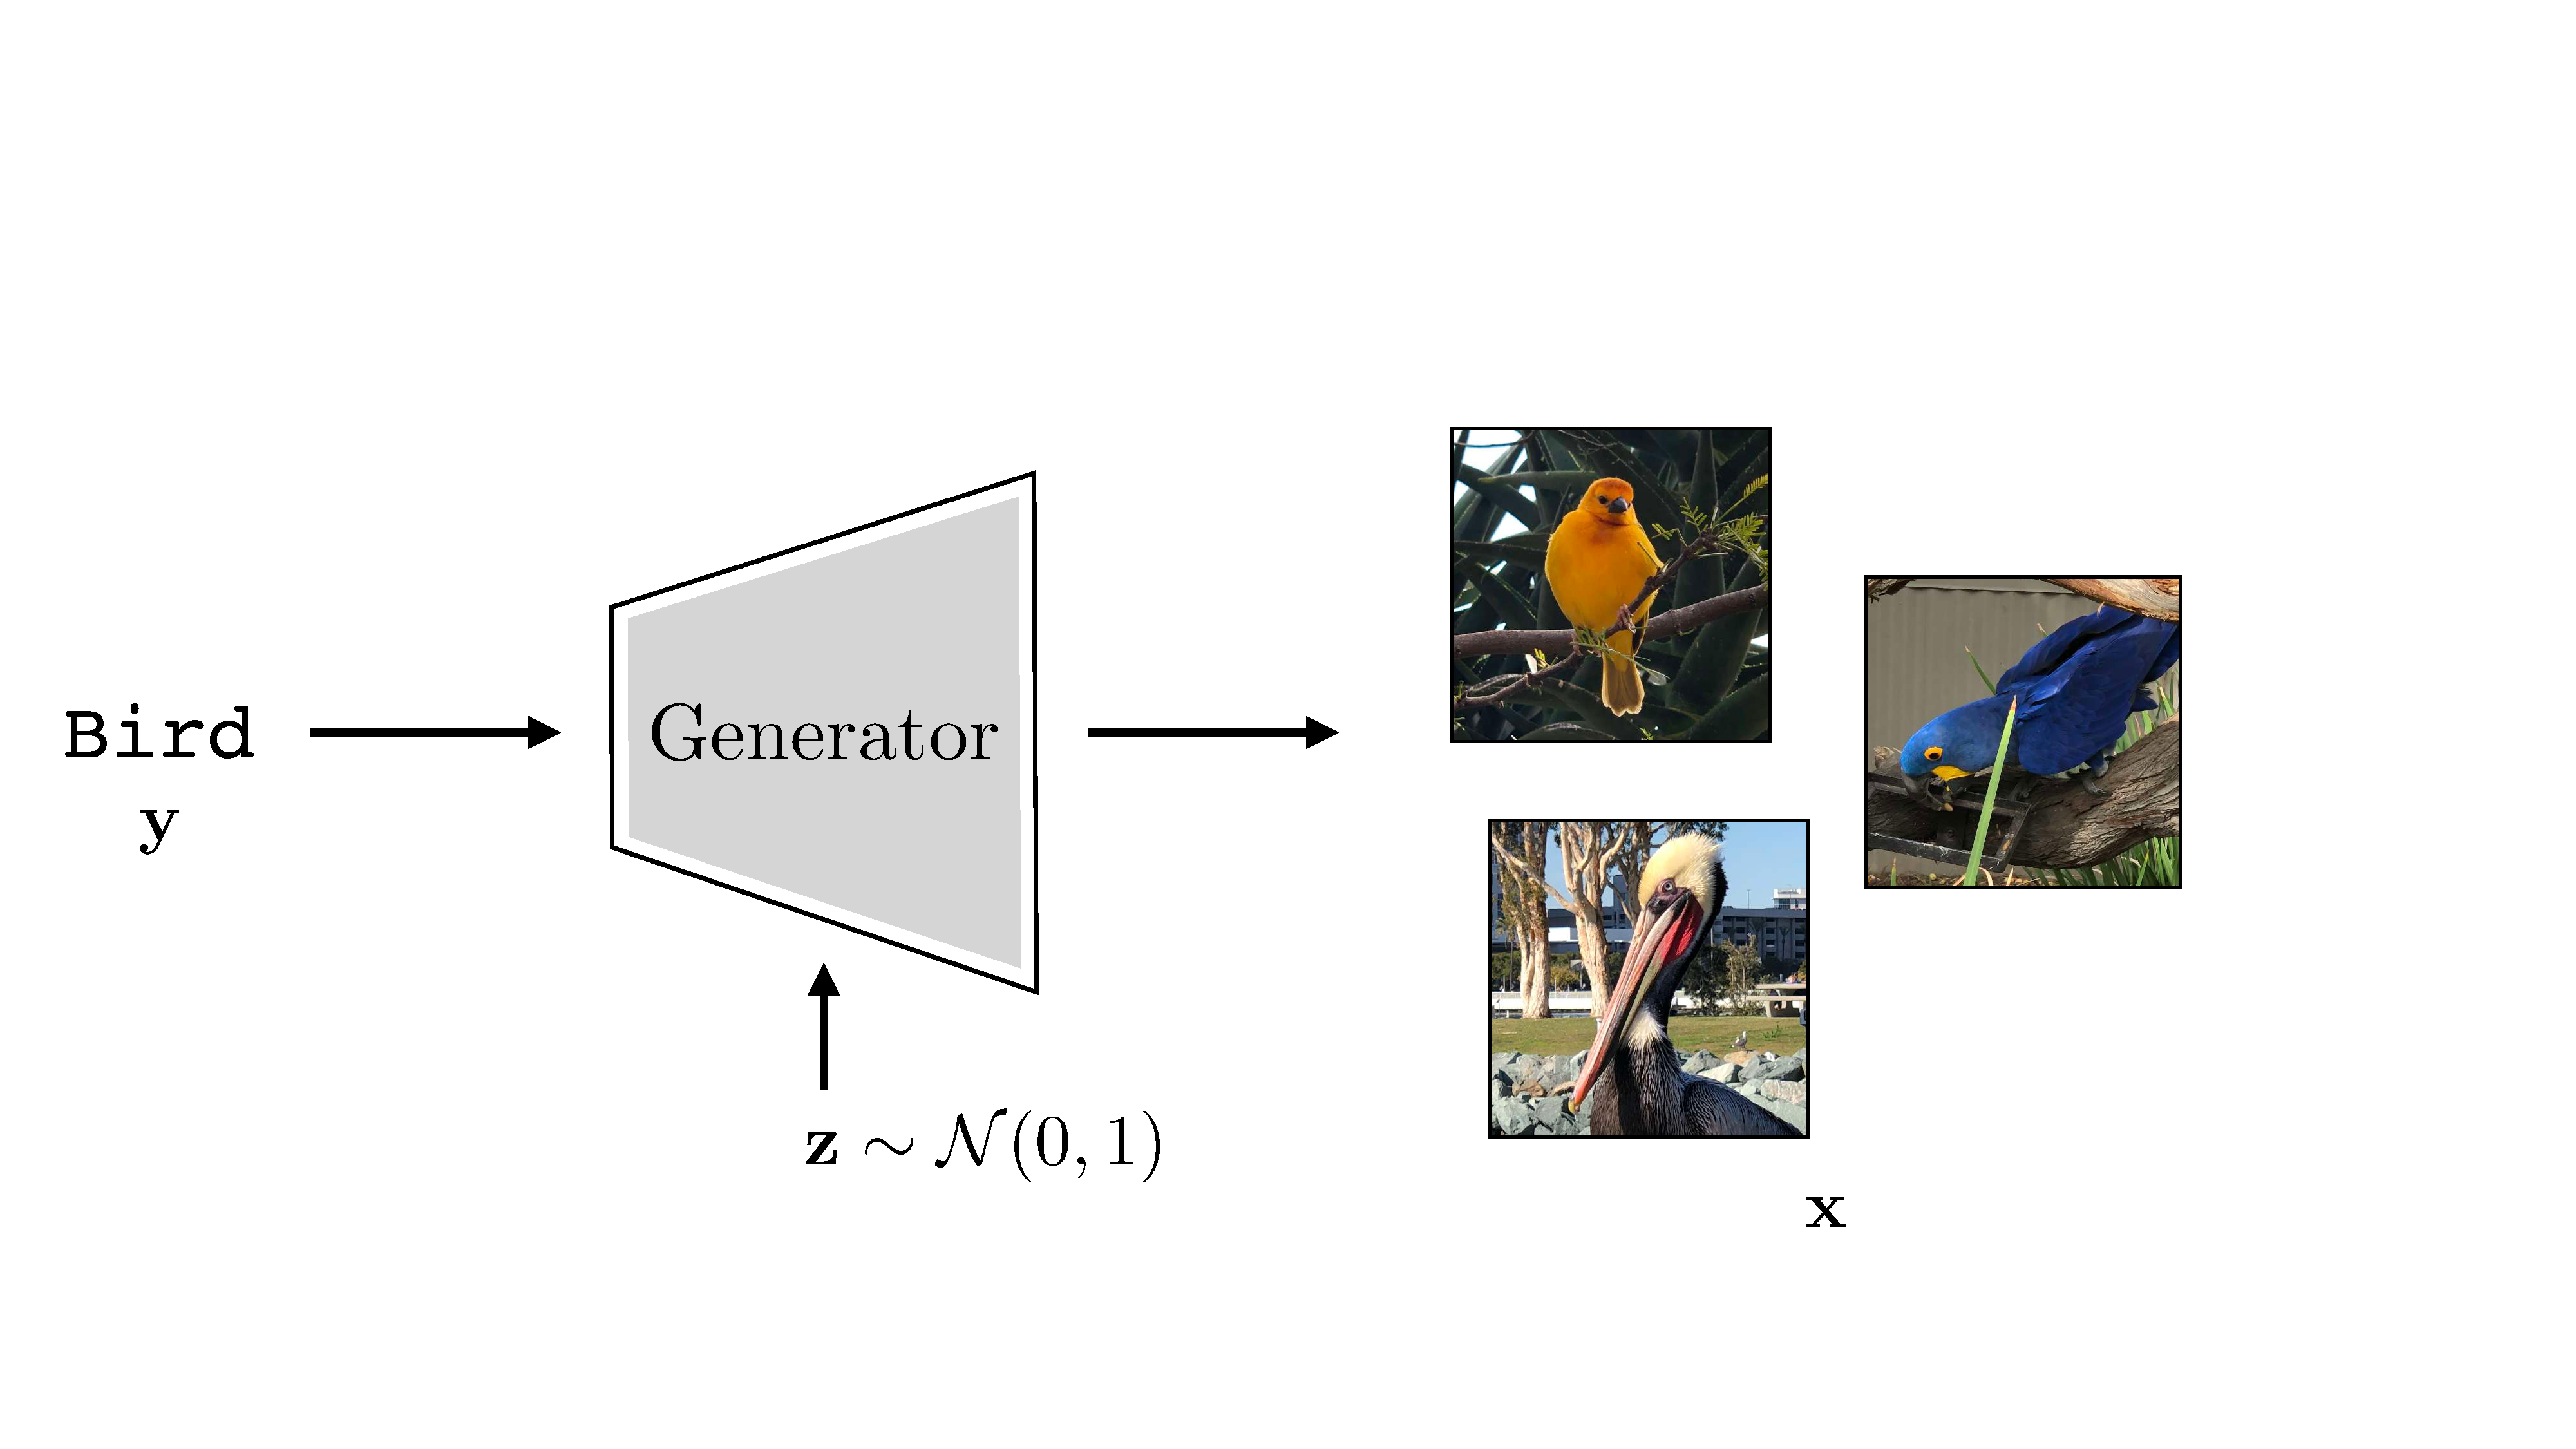
\includegraphics[width=0.7\linewidth]{./figures/generative_models/image_generation_with_z_birds.pdf}
    }
    \caption{Making a generator stochastic by conditioning on a random variable.}
    \label{fig:generative_models:image_generation_with_z}
\end{figure}

Usually we draw $\mathbf{z}$ from a simple distribution such as Gaussian noise, that is, $p(Z) = \mathcal{N}(\mathbf{0},\mathbf{1})$. The way to think of $\mathbf{z}$ is that it is a vector of \index{Latent variables}\textbf{latent variables}, which specify all the attributes of the images other than those determined by the label. These variables are called latent because they are not directly observed in the training data (it just consists of images $\mathbf{x}$ and their labels $\mathbf{y}$). %The $\mathbf{z}$-vector specifies all attributes of the generated image other than those determined by the input information $\mathbf{y}$. 
In our example, $\mathbf{y}$ tells $g$ to make a bird but the $\mathbf{z}$-vector is what specifies exactly which bird. Different dimensions of $\mathbf{z}$ specify different attributes, such as the size, color, pose, background, and so on; everything necessary to fully determine the output image.\marginnote{The $\mathbf{z}$-vector is also sometimes called \textbf{noise}, but noise has a very different meaning here than in signal processing. In signal processing, noise is a nuisance to get rid of. In generative modeling, \textit{the noise is the signal}; it determines exactly which image to generate.}[-3.1cm]% The same word is used because in both cases the ``noise'' is a random variable with a simple distribution (e.g., isotropic Gaussian).}[-3.2cm]

\section{Unconditional Generative Models}
\index{Generative models!Unconditional}
Sometimes we wish to simply make up data from scratch; in fact, this is the canonical setting in which generative models are often studied. To do so, we can simply drop the dependency on the input $\mathbf{y}$. This yields a procedure for making data from scratch:
\begin{align}
    \mathbf{z} \sim p(Z)\\
    \mathbf{x} = g(\mathbf{z})
\end{align}
\marginnote{Graphical model for an unconditional generative model:\\[6pt]
   \centering
   \includegraphics[width=0.06\linewidth]{./figures/generative_models/graphical_model_z_to_x_white.eps}
}[-1.8cm]
%This defines $\mathbf{x}$ as a random variable constructed by transforming random noise $\mathbf{z}$ through a deterministic function $g$. 
%In this form of generative modeling, our goal is to learn $g$ such that the distribution of random variable $\mathbf{x}$ matches some target distribution.
We call this an \textbf{unconditional generative model} because it is model of the unconditional distribution $p(X)$. Generally we will refer to unconditional generative models simply as generative models and use the term \textbf{conditional generative model} for a model of any conditional distribution $p(X \given Y)$. Conditional generative models will be the focus of \chap{\ref{chapter:conditional_generative_models}}; in the present chapter we will restrict our attention, from this point on, to unconditional models.

Why bother with (unconditional) generative models, which make up random synthetic data? At first this may seem a silly goal. Why should we care to make up images from scratch? One reason is \emph{content creation}; we will see other reasons later, but content creation is a good starting point. Suppose we are making a video game and we want to automatically generate a bunch of exciting levels for the player the explore. We would like a procedure for making up new levels from scratch. Such \index{Procedural graphics}{\bf procedural graphics} have been successfully used to generate random landscapes and cities for virtual realities~\cite{parish2001procedural}. Suppose we want to add a river to a landscape. We need to decide what path the river should take. A simple program for generating the path could be ``walk an increment forward, flip a coin to decide whether to turn left or right, repeat.'' 

\newpage
Here is that program in pseudocode:
%Here is a simple program that can make the decisions for us, automating the generation of river paths:
\begin{algorithm}[h]
\SetAlgoVlined
\DontPrintSemicolon
%\marginnote{{\bf Algorithm \ref{alg:generative_models:simple_rivers_script}}: A simple generative model that draws images of rivers.}
\caption{{\bf Algorithm \ref{alg:generative_models:simple_rivers_script}}: A simple generative model that draws images of rivers.}
\fakealgorithmcaption{}
\label{alg:generative_models:simple_rivers_script}
{\bf Input:} Random vector of coin flips $\mathbf{z} = [z_1, \ldots, z_{n}]$ with each $z_i \in \{0,1\}$\;
{\bf Output:} Picture of a river\;
\texttt{start drawing at origin with heading = $90^\circ$}\;
\For{\upshape $i=1, \dots, n$} {
    \texttt{extend line 1 unit in current heading direction}\;
    \If {$z_i==1$} {
        \texttt{rotate heading $10^\circ$ to the right}
    }
    \Else {
        \texttt{rotate heading $10^\circ$ to the left}
    }
}
\end{algorithm}

Here are a few rivers this program draws (\fig{\ref{fig:generative_models:rivers1}}):
\begin{figure}[h]
    \centerline{
    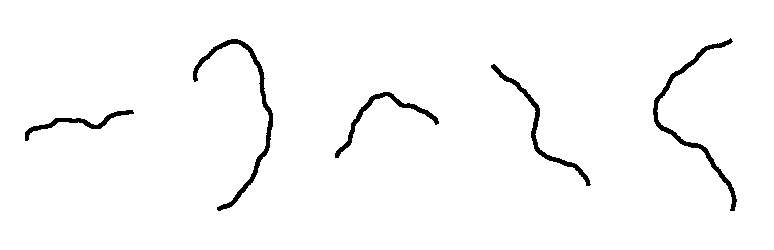
\includegraphics[width=0.8\linewidth]{./figures/generative_models/G4_river.pdf}
    }
    \caption{Procedurally generated rivers.}
    \label{fig:generative_models:rivers1}
\end{figure}

This program relies on a sequence of coin flips to generate the path of the river. In other words, the program took a randomized vector (noise) as input, and converted this vector into an image of the path of the river. It's exactly the same idea as we described previously for generating images of birds, just this time the generator is a program that makes rivers (\fig{\ref{fig:generative_models:gen_model_of_rivers_diagram}}):%\marginnote{In the context of generative models, the term \textbf{noise} has a very different meaning than in the context of signal processing, which you may be more familiar with. In signal processing, we think of noise as a nuisance to get rid of. In generative modeling, noise refers to the disentangled factors of variation input to the model, which affect how an image will look. The same word is used because in both cases the ``noise'' is a random variable with a simple distribution (e.g., isotropic Gaussian).}[-1cm]
\begin{figure}[h]
    \centerline{
    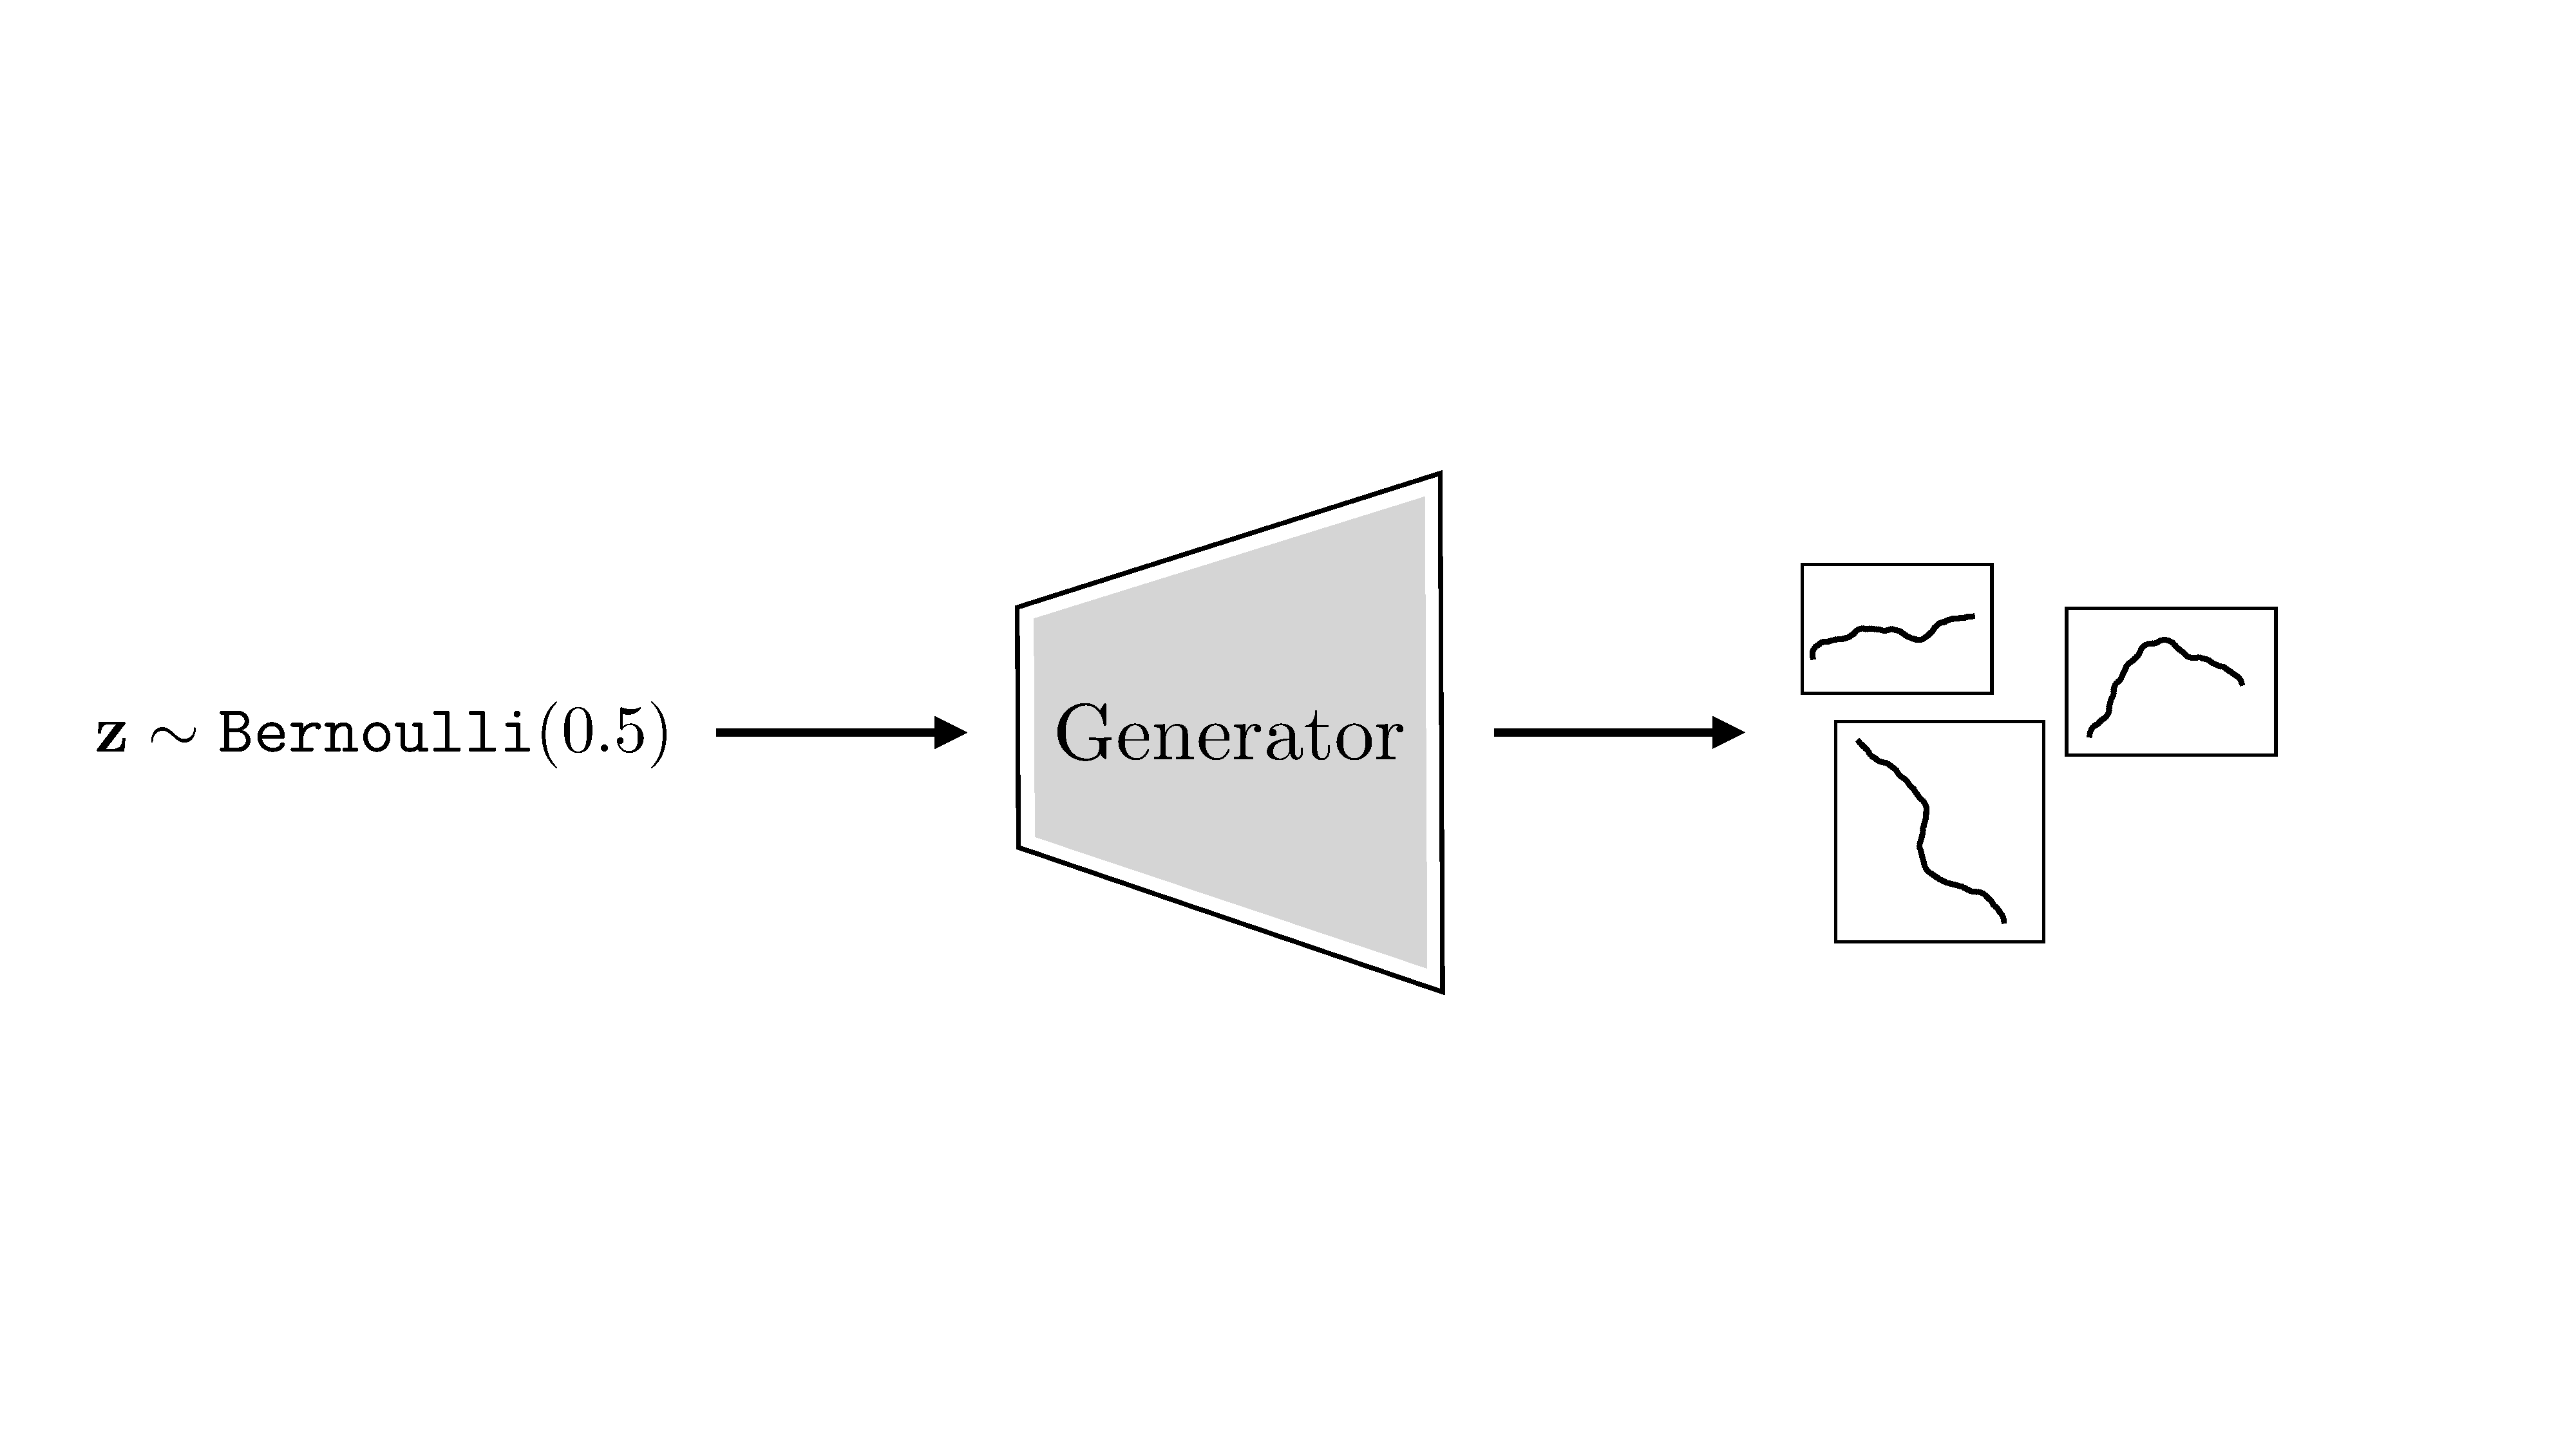
\includegraphics[width=0.75\linewidth]{./figures/generative_models/gen_model_of_rivers_diagram.pdf}
    }
    \caption{A generator that makes procedural rivers.}
    \label{fig:generative_models:gen_model_of_rivers_diagram}
\end{figure}

This generator was written by hand. Next we will see generative models that \textit{learn} the program that synthesizes data.%, by setting its parameters such that the output matches some target distribution, for example, we may wish the output to match the distribution of actual river paths in the wild.
%Imagination.

\section{Learning Generative Models}
How can we learn to synthesize images that look realistic? The machine learning way to do this is to start with a training set of \textit{examples} of real images, $\{\mathbf{x}^{(i)}\}_{i=1}^N$. Recall that in supervised learning, an \textit{example} was defined as an \{\texttt{input}, \texttt{output}\} pair; here things are actually no different, only the \texttt{input} happens to be the null set. We feed these examples to a learner, which spits out a generator function. Later, we may query the generator with new, randomized $\mathbf{z}$-vectors to produce novel outputs, a process called \index{Sampling}\textbf{sampling} from the model. This two-stage procedure is shown in \fig{\ref{fig:generative_models:gen_model_training_vs_sampling}}:
\begin{figure}[h]
    \centerline{
    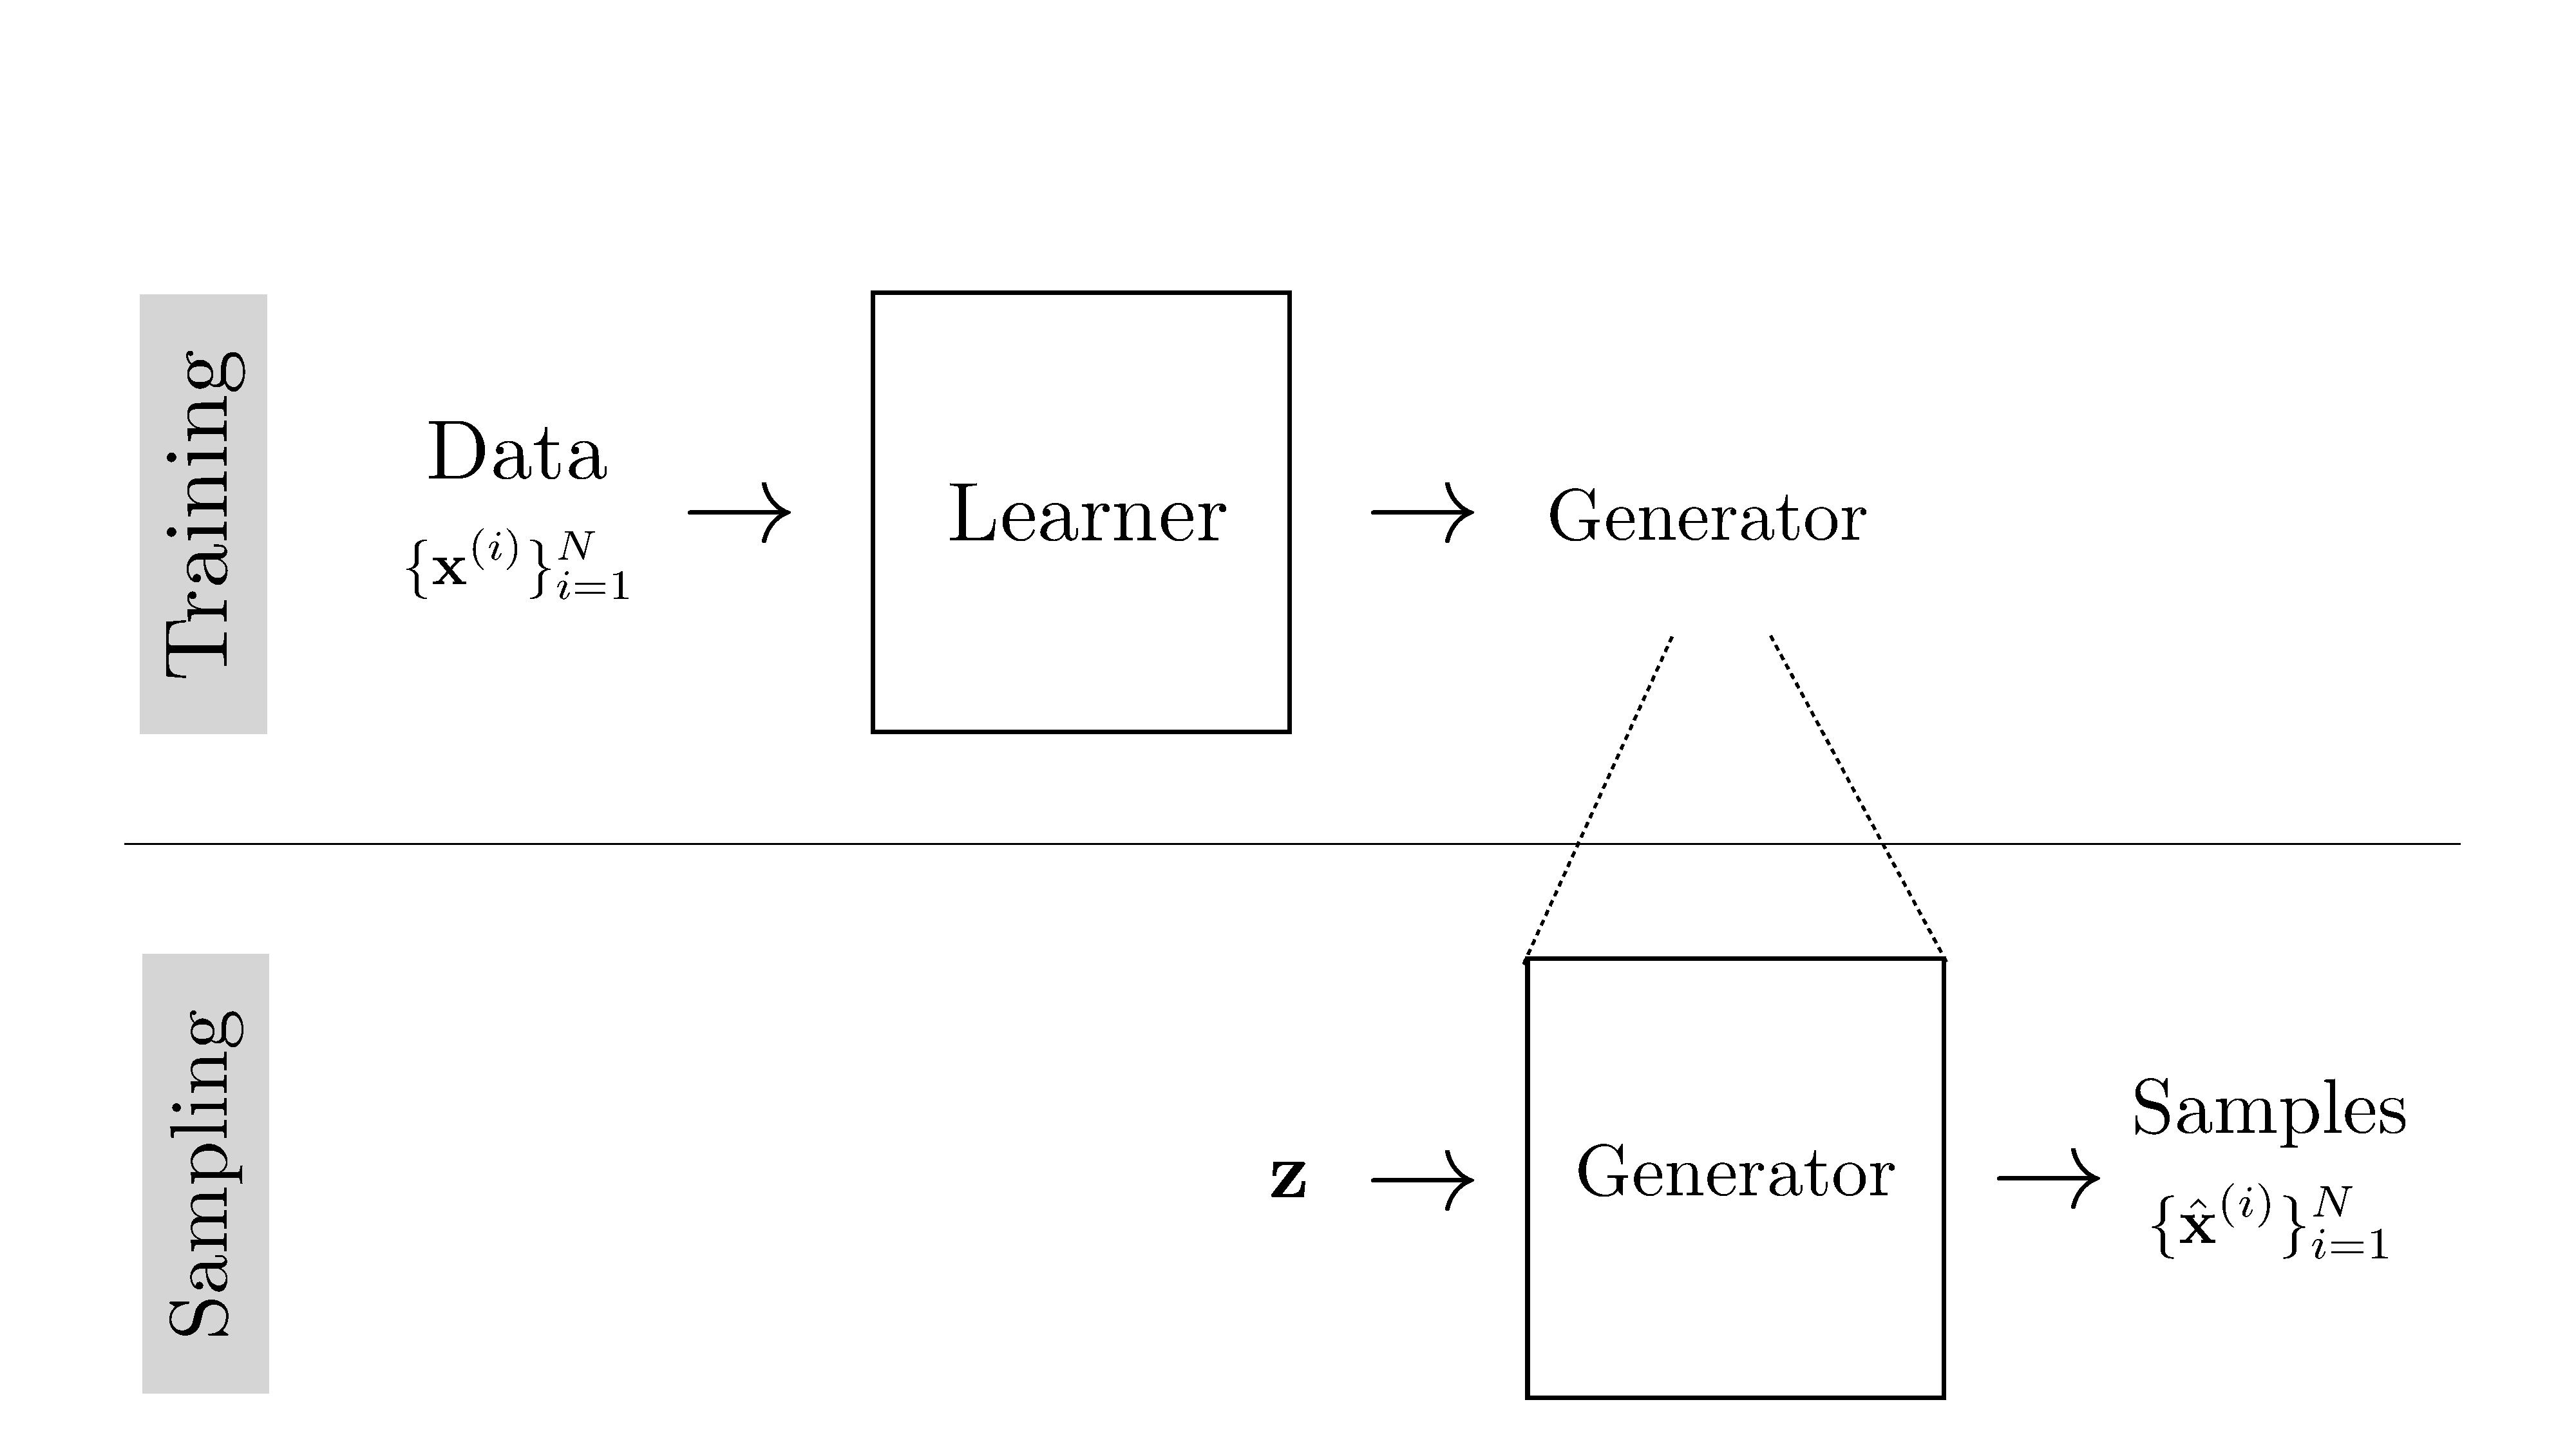
\includegraphics[width=0.9\linewidth]{./figures/generative_models/gen_model_training_vs_sampling.pdf}
    }
    \caption{Learning and using a generator.}
    \label{fig:generative_models:gen_model_training_vs_sampling}
\end{figure}

\subsection{What's the Objective of Generative Modeling?}
The objective of the learner is to create a generator that produces \textit{synthetic} data, $\{\hat{\mathbf{x}}^{(i)}\}_{i=1}^N$, that looks like the \textit{real} data, $\{\mathbf{x}^{(i)}\}_{i=1}^N$. There are a lot of ways of define ``looks like'' and they each result in a different kind of generative model. Two examples are:
\begin{enumerate}
    \item Synthetic data looks like real data if matches the real data in terms of certain marginal statistics, for example, it has the same mean color as real photos, or the same color variance, or the same edge statistics.
    \item Synthetic data looks like real data if it has high probability under a density model fit to the real data.
\end{enumerate}
The first approach is the one we saw in \chap{\ref{chapter:stat_image_models}} on statistical image models, where synthetic textures were made that had the same filter response statistics as a real training example. This approach works well when we only want to match certain properties of the training data. The second approach, which is the main focus of this chapter, is better when we want to produce synthetic data that matches \textit{all} statistics of the training examples.\footnote{In practice, we may not be able to match all statistics, due to limits of the model's capacity.}

To be precise, the goal of the deep generative models we consider in this chapter is to produce synthetic data that is \textit{identically distributed} as the training data, that is, we want $\hat{\mathbf{x}} \sim p_{\texttt{data}}$ where $p_{\texttt{data}}$ is the true process that produced the training data. %We will see several ways to achieve this in the following sections.

What if our model just memorizes all the training examples and generates random draws from this memory? Indeed, memorized training samples perfectly satisfy the goal of making synthetic data that looks real. A second, sometimes overlooked, property of a good generative model is that it be a simple, or smooth, function, so that it generalizes to producing synthetic samples that look like the training data but are not identical to it. A generator that only regurgitates the training data is overfit in the same way a classifier that memorizes the training data is overfit. In both cases, the true goal is to fit the training data and to do so with a function that generalizes.

\subsection{The Direct Approach and the Indirect Approach}
There are two general approaches to forming data generators:
\begin{enumerate}
    \item Direct approach: learn the function $G: \mathcal{Z} \rightarrow \mathcal{X}$.
    \item Indirect approach: learn a function $E: \mathcal{X} \rightarrow \mathbb{R}$ and generate samples by finding values for $\mathbf{x}$ that score highly under this function.
\end{enumerate}
\marginnote{In the generative modeling literature, the direct approach is sometimes called an \textit{implicit} model. This is because the probability density is never explicitly represented. However, note that this ``implicit'' model explicitly describes the way data is generated. To avoid confusion, we will not use this terminology.}[-2cm]
So far in this chapter we have focused on the direct approach, and it is schematized in \fig{\ref{fig:generative_models:gen_model_training_vs_sampling}}. Interestingly, the direct approach only became popular recently, with models like \textbf{generative adversarial networks} (\textbf{GANs}) and \textbf{diffusion models}, which we will see later in this chapter. The indirect approach is more classical, and describes many of the methods we saw in \chap{\ref{chapter:stat_image_models}}. Indirect approaches come in two general flavors, density models and energy models, which we will describe next. Both follow the schematic given in \fig{\ref{fig:generative_models:gen_model_training_vs_sampling_indirect}}:
\begin{figure}[h]
    \centerline{
    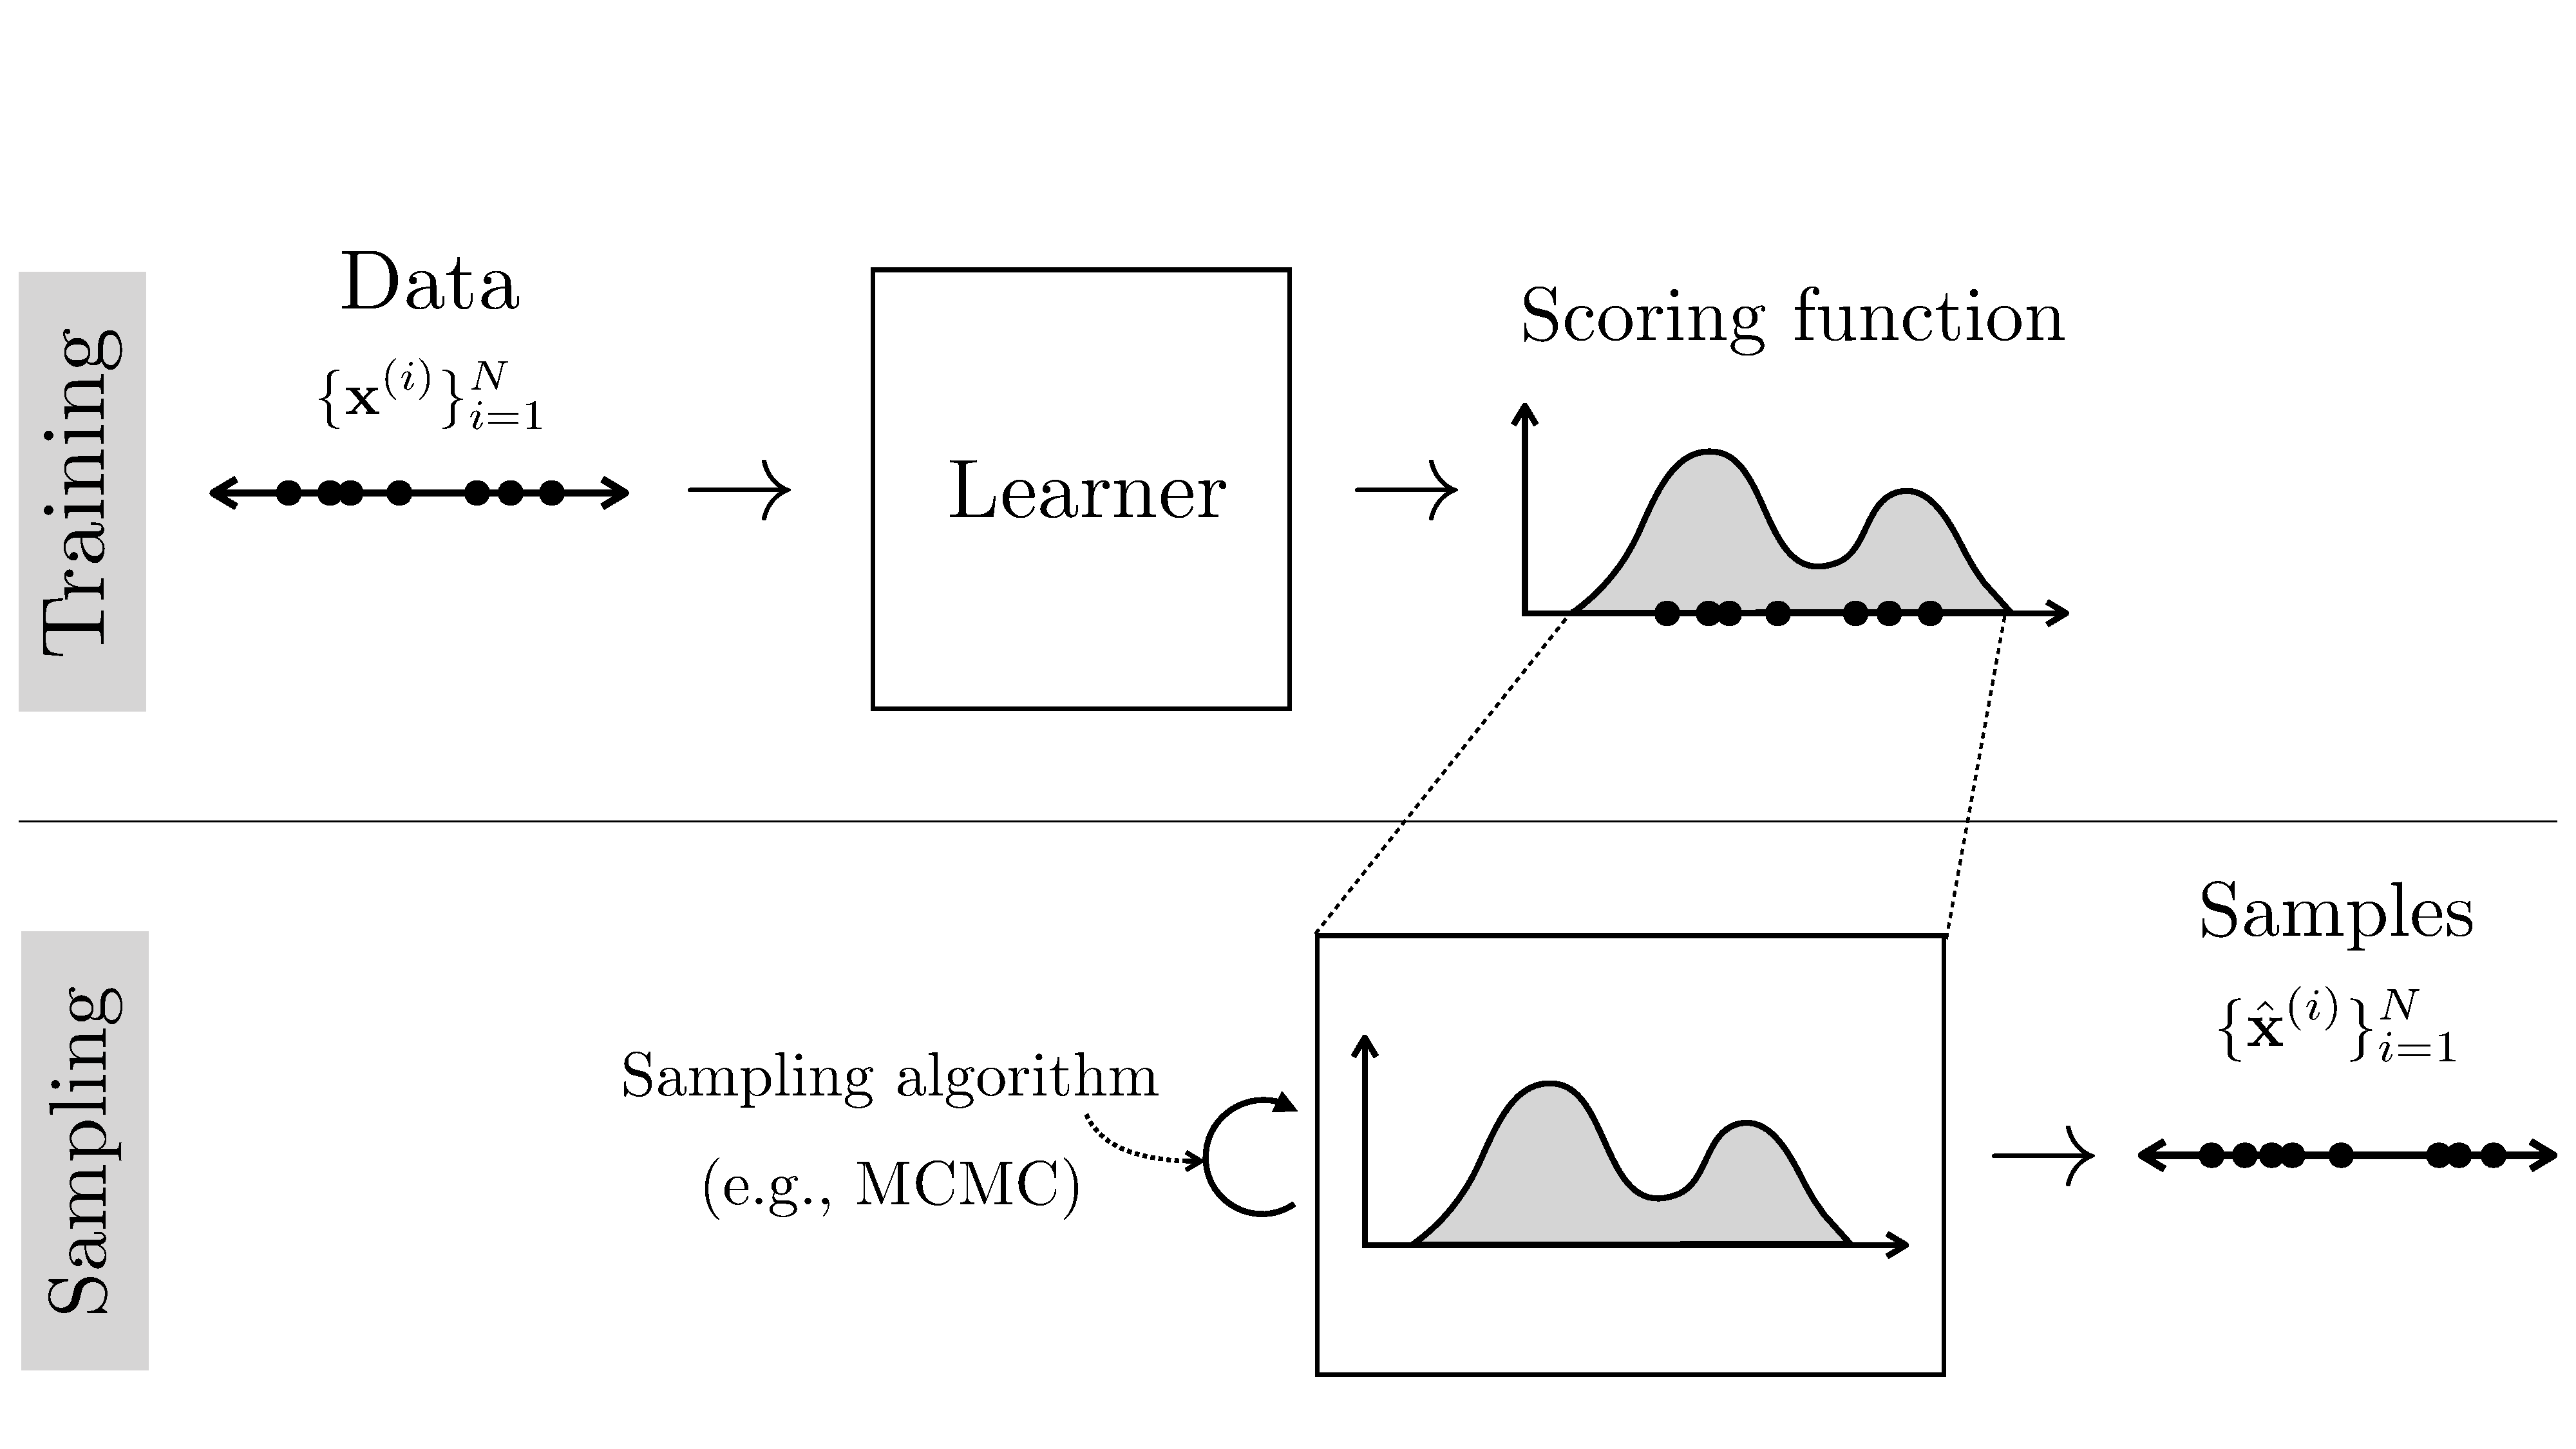
\includegraphics[width=1.0\linewidth]{./figures/generative_models/gen_model_training_vs_sampling_indirect.pdf}
    }
    \caption{The indirect approach to generative modeling. The scoring function can be either a probability density or an energy function. The models we learned about in \chap{\ref{chapter:stat_image_models}} follow this recipe (see \figs{\ref{fig:model_training_vs_sampling}} and \ref{fig:model_hist_example} in particular).}
    \label{fig:generative_models:gen_model_training_vs_sampling_indirect}
\end{figure}

%An example of the direct approach is the \textbf{Generative Adversarial Network} that we will see later in this chapter. First, however, we will describe the more classical, indirect approach in the following sections. Indirect approaches come in two general flavors, density models and energy models, which we describe next.
%\marginnote{The vocabulary for these different approaches can be confusing. In the generative modeling literature, the direct approach is sometimes called an \textit{implicit} model because the probability density is never explicitly represented. However, this usage contrasts with the more usual use of ``implicit functions" in math: $y = f(x)$ is explicit while $y = \argmin_y E(x,y)$ is ``implicit" as the output is the implied result of an optimization procedure over $E$, rather than the direct result of running a function $f$. The indirect approach to generative modeling is ``implicit" in that the output is a sampling procedure over a density or energy function

\section{Density Models}
\index{Density model}
Some generative models not only produce generators but also yield a probability density function $p_{\theta}$, fit to the training data. This density function may play a role in training the generator (e.g., we want the generator to produce samples from $p_{\theta}$), or the density function may be the goal itself (e.g., we want to be able to estimate the probability of datapoints in order to detect anomalies).

In fact, some generative models \textit{only} produce a density $p_{\theta}$ and do not learn any explicit generator function. Instead, samples can be drawn from $p_{\theta}$ using a sampling algorithm, such as \textbf{Markov Chain Monte Carlo} (\textbf{MCMC}), that takes a density as input and produce samples from it as output. This is a form of the indirect approach to synthesizing data that we mentioned above (\fig{\ref{fig:generative_models:gen_model_training_vs_sampling_indirect}}).

%Generative models that just produce a generator $G_{\theta}: \mathcal{Z} \rightarrow \mathcal{X}$ are sometimes called {\bf implicit generative models}, because they do not explicitly give us the likelihood (a.k.a. probability) of the samples they generate. Other generative models instead fit an explicit probability {\bf density} to the input data, $p_{\theta}: \mathcal{X} \rightarrow [0,1]$:\marginnote{It's unfortunate that history chose the term ``implicit" for generative models that give samples but not densities, and ``explicit" for generative models that give densities but not samples. We feel it would make more sense to swap the terms, and think of density models as implicitly defining a way of generating data, and samplers as explicitly defining a way of generating data, but alas that's not the accepted vocabulary.}[-1.3cm]

%A classical way to learn a generative model is to first fit a probability density function to the training data, then sample from this density. In 
%In this case, the ``Generator" in Figure \ref{fig:generative_models:gen_model_training_vs_sampling} is actually a program that repeatedly calls a density function as a subroutine. Sometimes the learned density model is itself called a generative model since it implicitly defines a way to generate data.\maginnote{Confusingly, generative models that skip the step of modeling a density function as sometimes called ``implicit" models, because the density is implied rather than explicit.}


%If we are given training data $\mathbf{x} \sim p_{\texttt{data}}$, our goal is to learn a {\bf generator} $G_{\theta}$ from this data such that $G_{\theta}$ produces synthetic data, $\hat{\mathbf{x}}$ that \textit{looks like the training data}. There are a lot of ways of define ``looks like'' and they each result in a different kind of generative model.

%We will define the function that checks if the outputs of a generator ``look like" the training data to be called a {\bf critic}. \marginnote{``Critic" is not a standard term in in this context; we are borrowing it from ``actor-critic" methods in reinforcement learning. In the context of generative models, the actor is the generator and the critic is either a likelihood function, an energy function, or a discriminator function, depending on the type of model.} The critic takes one or more generated images as input and scores them; we call images output by the generated as \textbf{fake} images, and those sampled from the training data as \textbf{real} images. The goal of the generator is to produce images that score highly under the critic, and the goal of the critic is to assign high scores to realistic images. In Chapter XX, we already saw one example of a generator and a critic: the Heeger \& Bergen model uses a critic that checks if a fake texture has the same filter response statistics as a real texture example. The generator is then a procedure that iteratively projects random noise into the subspace with features that satisfy the critic.

%The first thing to note is that we do not, typically, care to make fake images that are exact copy of the training data, identical in every way. Instead, we want to make fake data that matches some desired properties of the training data, but is otherwise randomized. Generically, therefore, the critic should not check if the fake images are identical to training images but instead that they match certain desired properties or statistics of the training data. For example, we may want to produce fake images that have the same \textit{mean} and \textit{variance} as the training data. 

%The most popular kinds of generative models aim to make synthetic data that has the same \textit{distribution} as the training data. For these models, one standard kind of critic is a density function. First we fit the density to the training data, then we sample from that density.

%The ``looks like" comparator is called a ``critic". The critic scores if an image has the same statistical properties as the training data, for example if it is likely to have come from the same distribution as the training data.

%Most generative models consist of two functions: a {\bf generator} and a {\bf critic}.\marginnote{``Critic" is not a standard term in in this context; we are borrowing it from ``actor-critic" methods in reinforcement learning. In the context of generative models, the actor is the generator and the critic is either a likelihood function, an energy function, or a discriminator function, depending on the type of model.} The critic is a function that checks if a candidate set of images is a set we like. The generator is a function that tries to make candidate images the critic will score highly.

%\marginnote{This is actually a common setup, often we have f* = argmin_f V(f), where V is a critic that evaluates how good a function is. We can either first learn V, then use optimization to get f*, or we can directly learn f* or can learn both simultaneously.}

%How can we learn to do this? If we are given training data $\mathbf{x} \sim p_{\texttt{data}}$, our goal is to learn $G_{\theta}$ from this data such that $G_{\theta}$ produces synthetic data, $\hat{\mathbf{x}}$ that \textit{looks like the training data}. There are a lot of ways of define ``looks like'' and they each result in a different kind of generative model. 

%The first thing to note is that we do not, typically, care to make synthetic data that is just an exact copy of the training data, identical in every way. Instead, we will make synthetic data that matches some desired properties of the training data, but is otherwise randomized. Generically, the desired properties will be summary statistics of the training data. For example, we may want to produce synthetic data that has the same \textit{mean} and \textit{variance} as the training data. The most popular kinds of generative models aim to make synthetic data that has the same \textit{distribution} as the training data.  %Remember, the distribution of the training data is a summary statistic of it. 
%Formally, we want our model to produce samples that are identically distributed as the training data, i.e. $\hat{\mathbf{x}} \sim p_{\texttt{data}}$:\footnote{the figures on this page and the next are derived from: \texttt{http://introtodeeplearning.com/materials/2019\_6S191\_L4.pdf}}

%\begin{figure}[h]
%    \centering
%    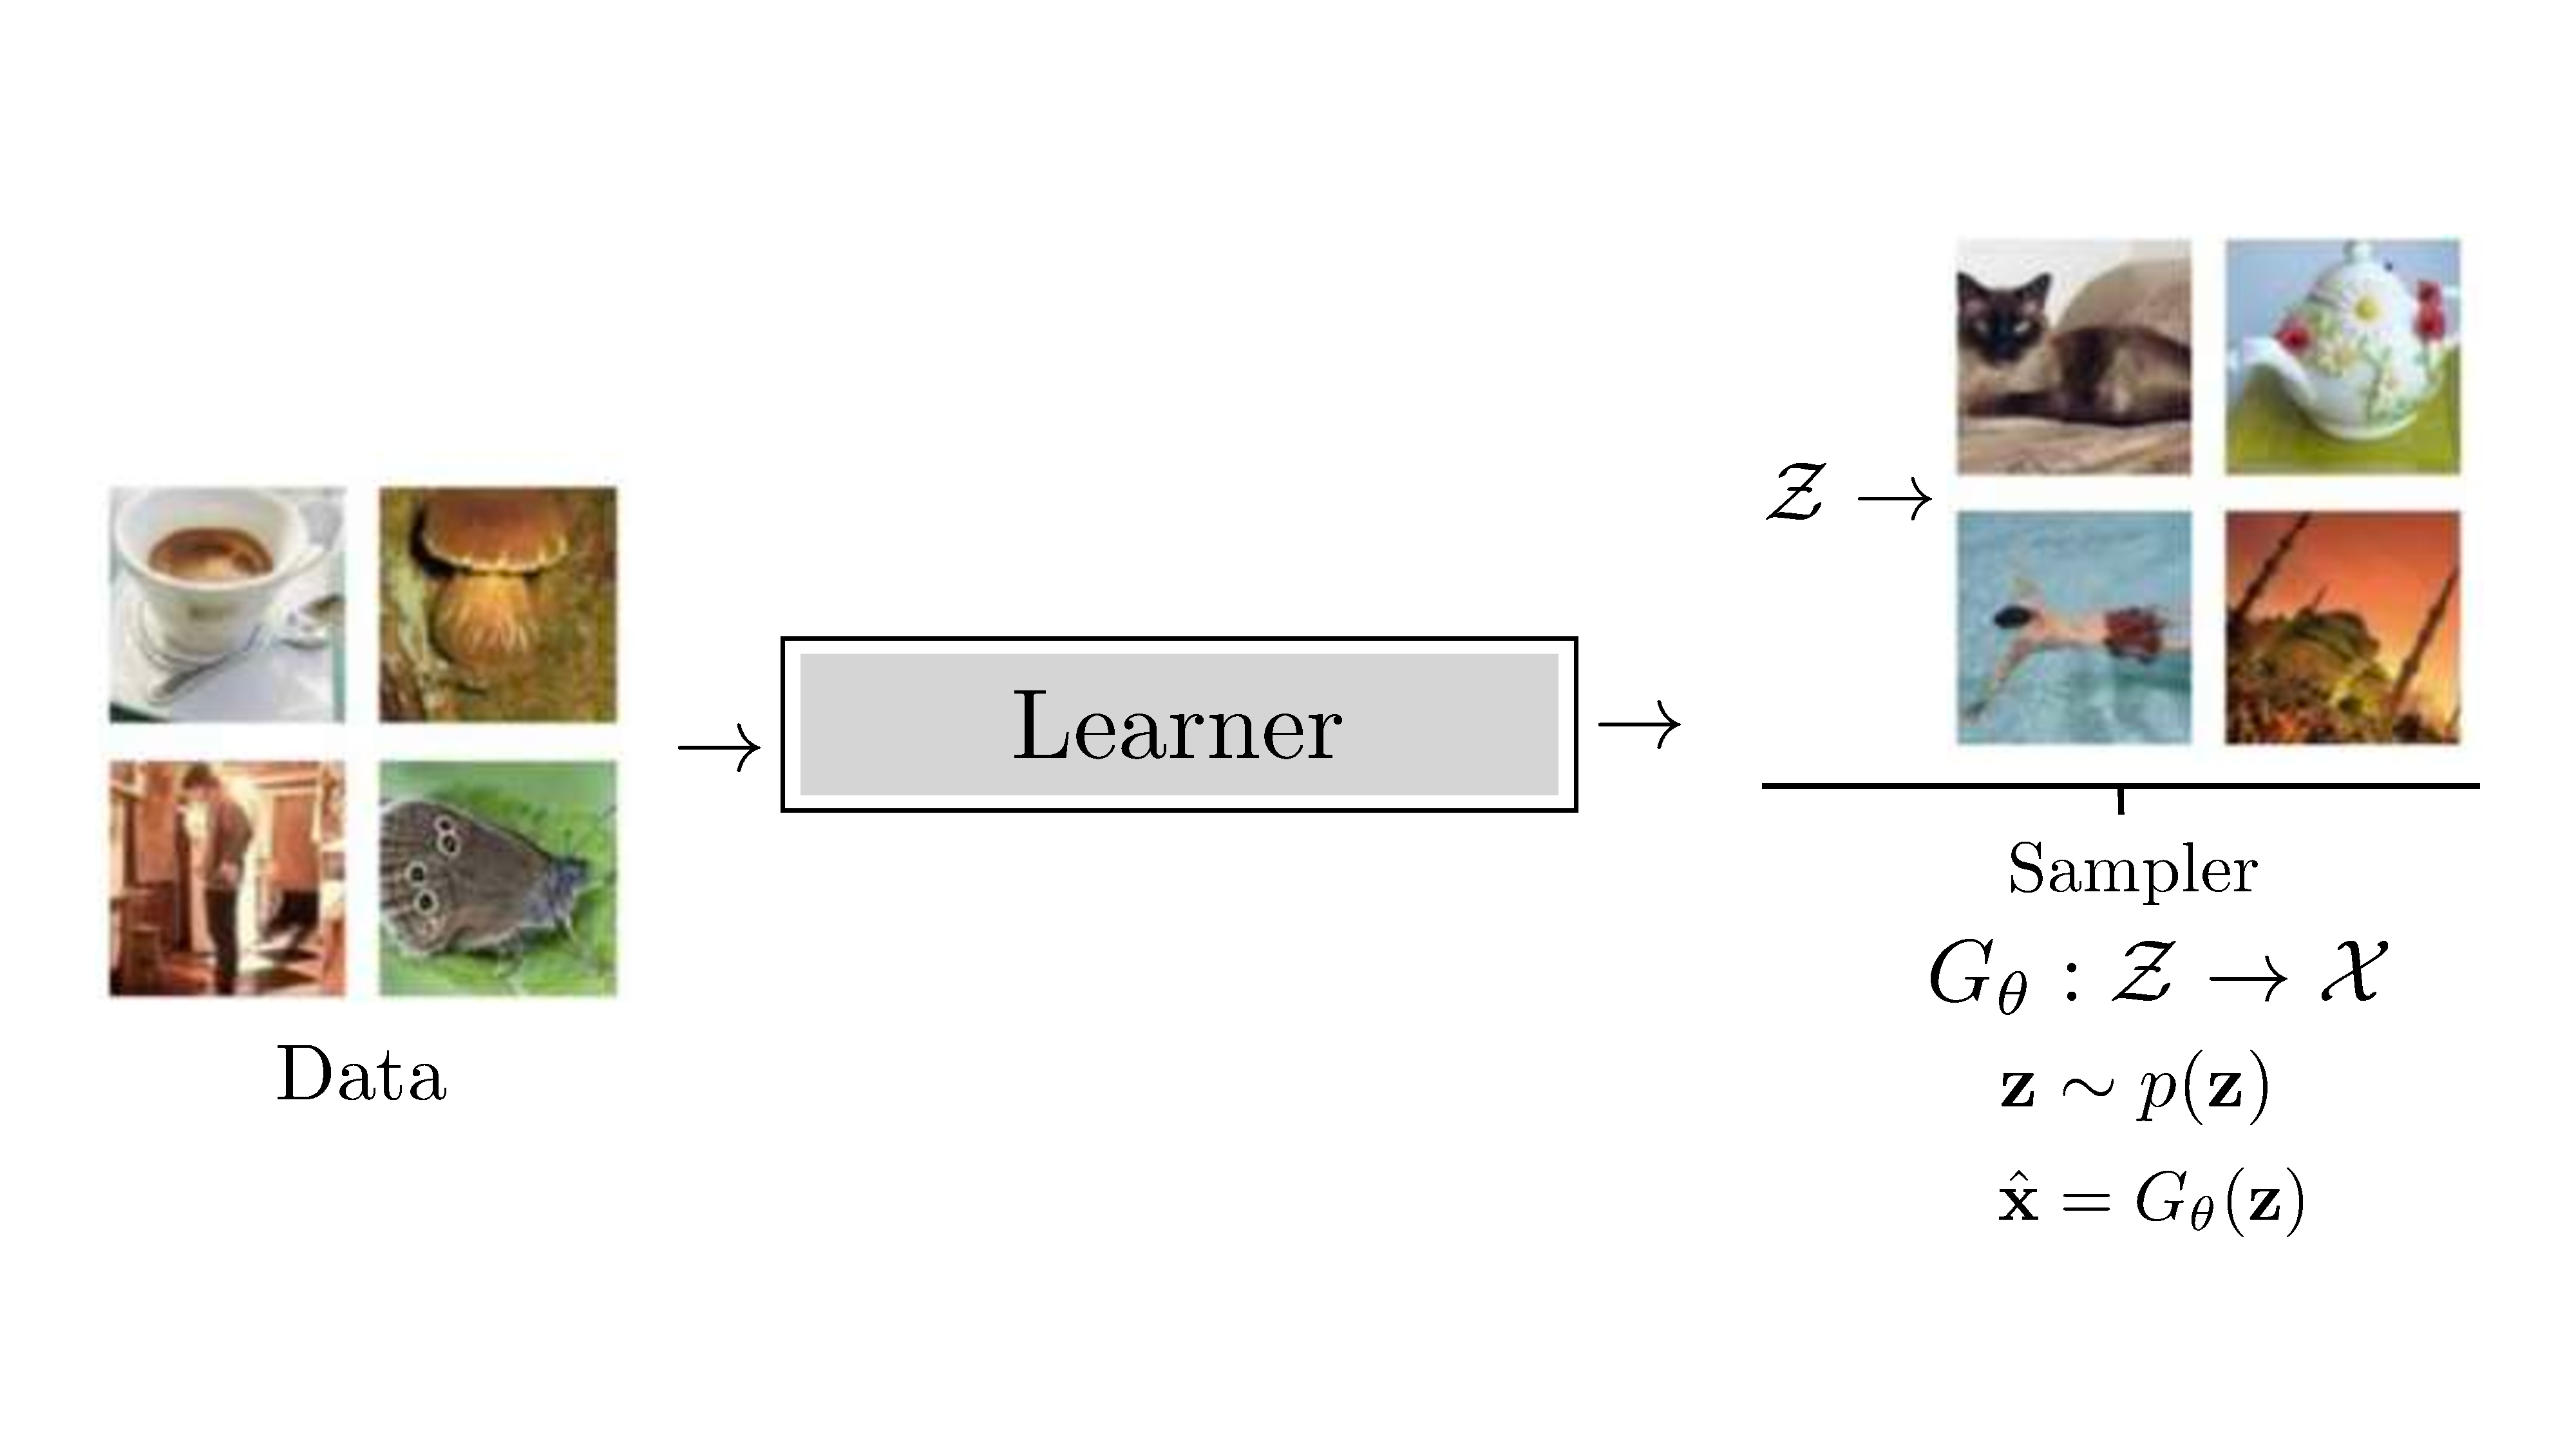
\includegraphics[width=0.9\linewidth]{./figures/generative_models/sampler_formalism.pdf}
%    \label{fig:sampler_formalism}
%\end{figure}

%Generative models that just produce a {\bf sampler} $G_{\theta}: \mathcal{Z} \rightarrow \mathcal{X}$ are sometimes called {\bf implicit generative models}, because they do not explicitly give us the likelihood (a.k.a. probability) of the samples they generate. Other generative models instead fit an explicit probability {\bf density} to the input data, $p_{\theta}: \mathcal{X} \rightarrow [0,1]$:\marginnote{It's unfortunate that history chose the term ``implicit" for generative models that give samples but not densities, and ``explicit" for generative models that give densities but not samples. We feel it would make more sense to swap the terms, and think of density models as implicitly defining a way of generating data, and samplers as explicitly defining a way of generating data, but alas that's not the accepted vocabulary.}[-1.3cm]

%A generative model \emph{learner} takes data $\{\mathbf{x}_i\}_{i=1}^N$ as input and outputs one of two things (or sometimes both): 1) a {\bf density} $p_{\theta}: \mathcal{X} \rightarrow [0,1]$, 2) a {\bf sampler} $g_{\theta}: \mathcal{Z} \rightarrow \mathcal{X}$ that maps random noise $z$ to data sample $x$, i.e. $x = g(z)$, $z \sim p(z)$, such that $x \sim p_{\texttt{data}}(x)$:

% \begin{figure}[h]
%     \centering
%     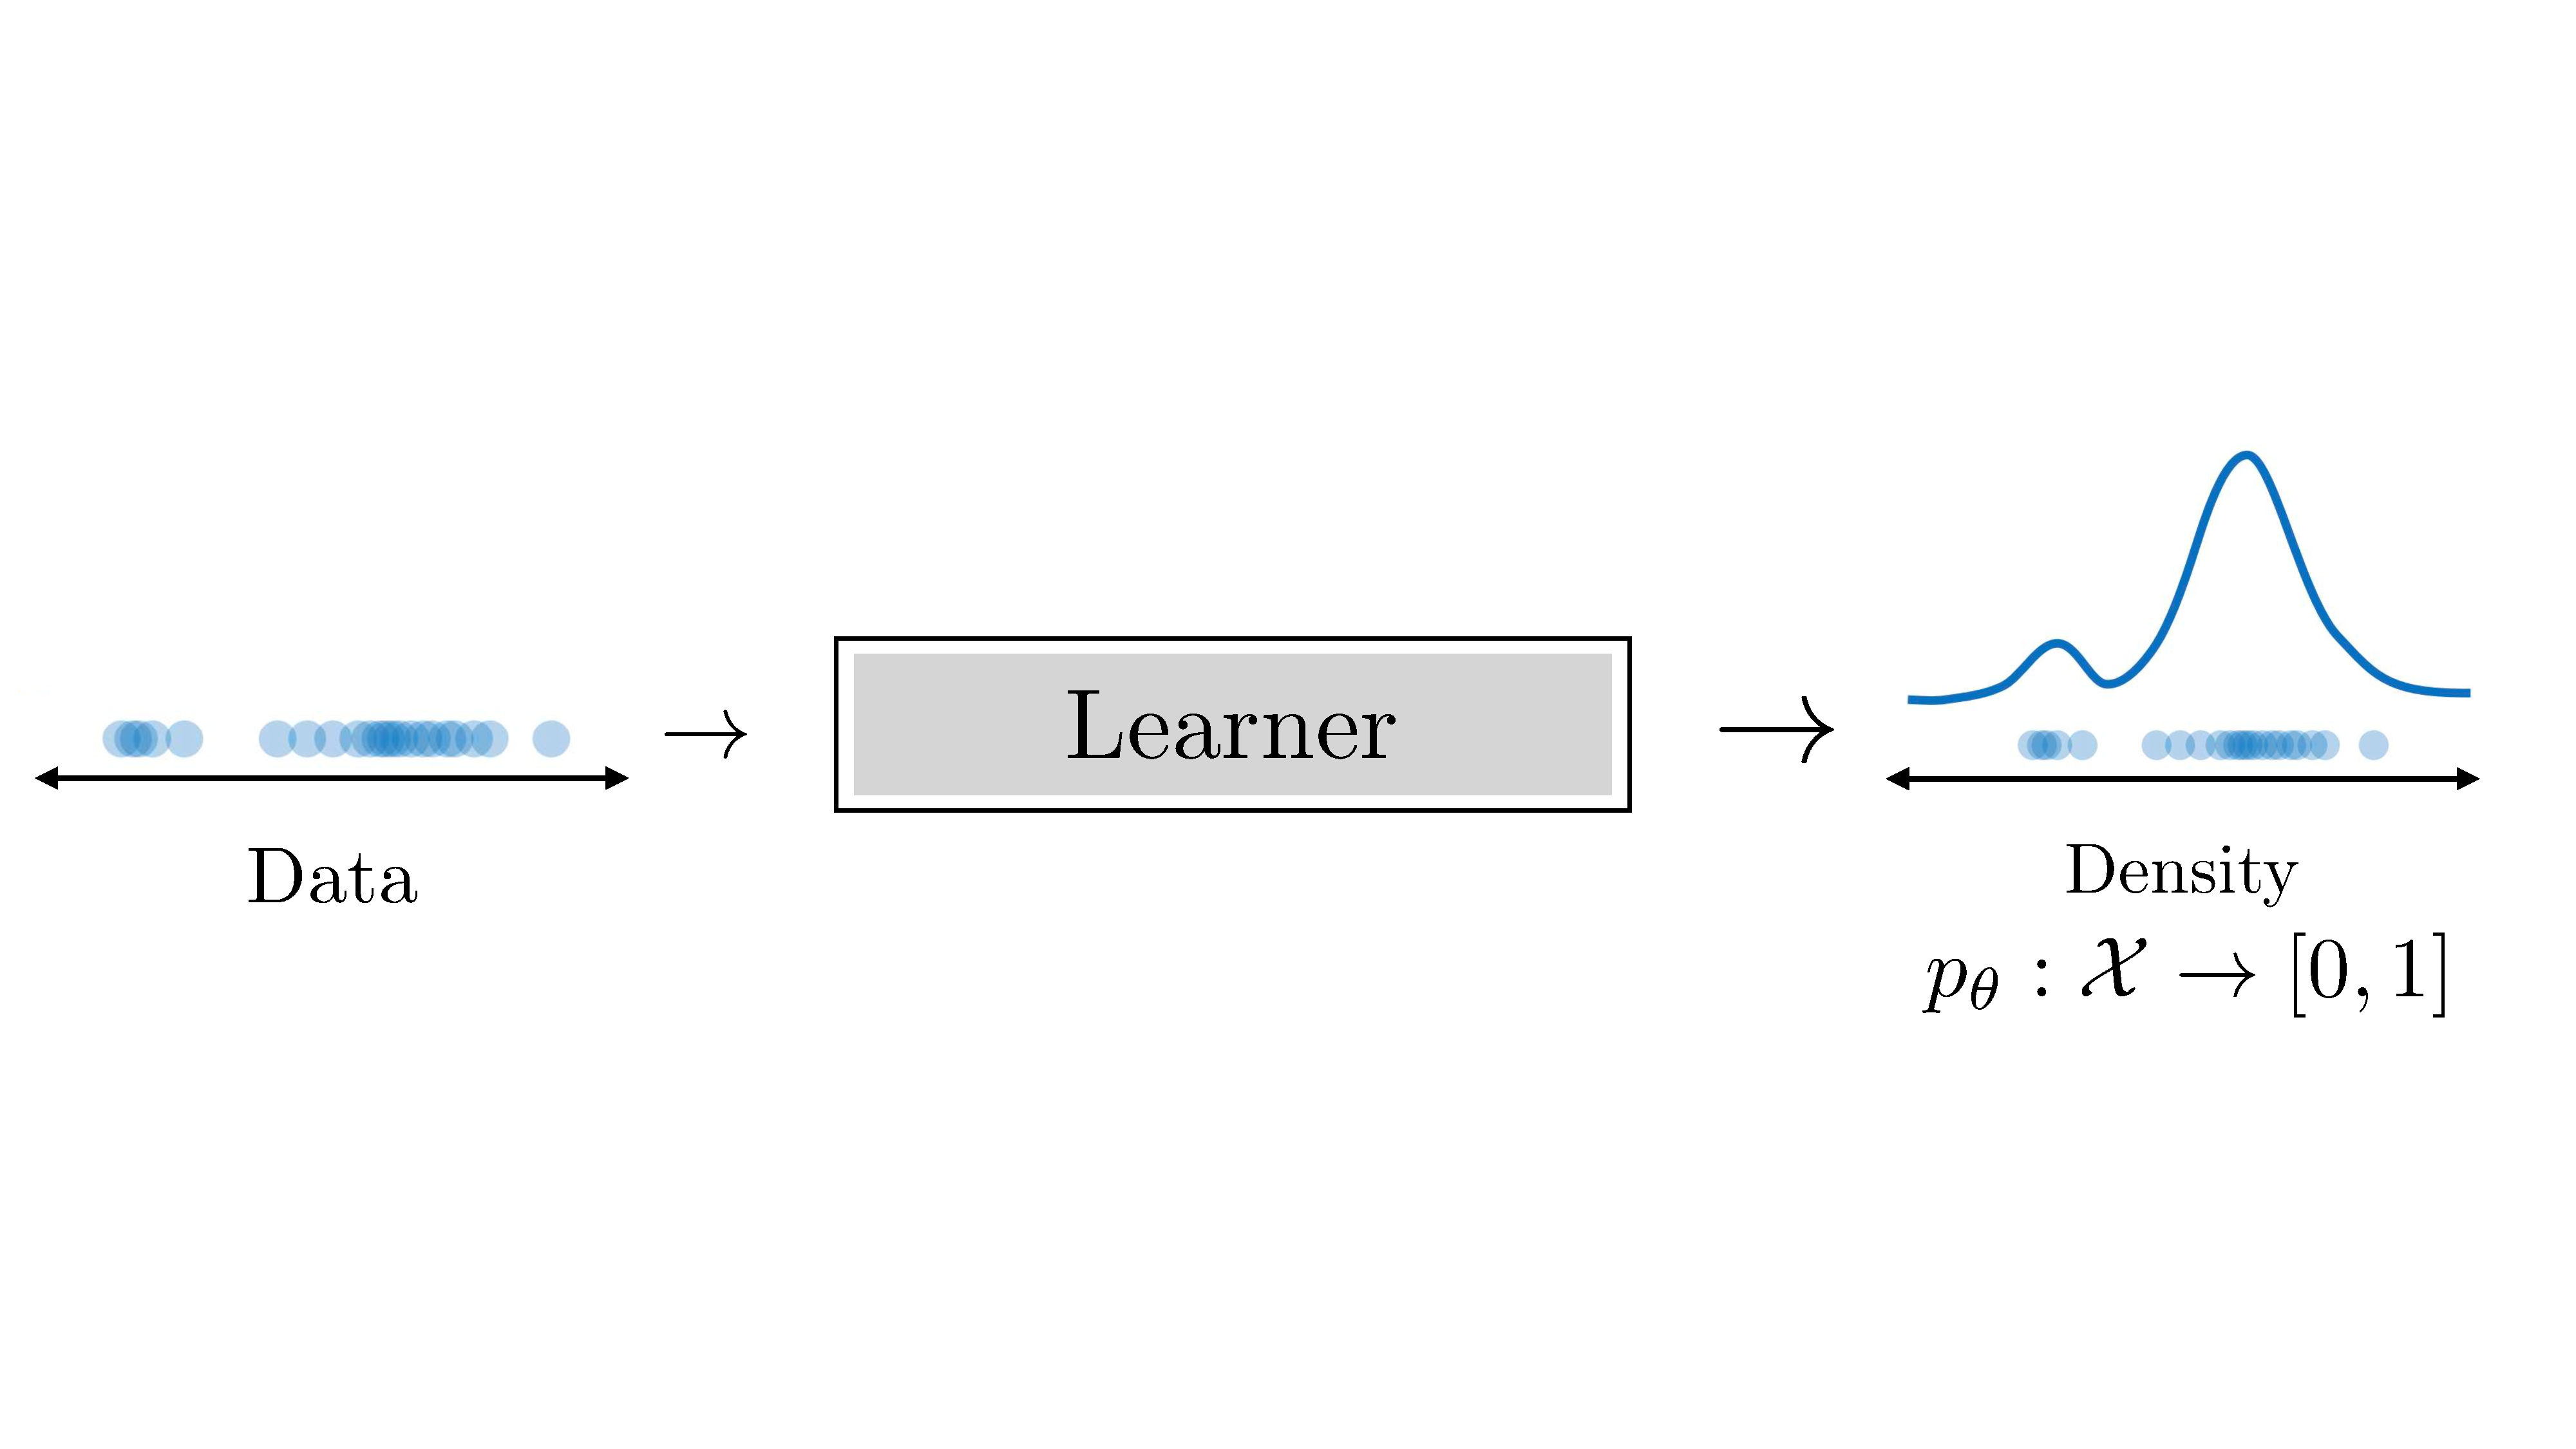
\includegraphics[width=0.9\linewidth]{./figures/generative_models/density_modeling_formalism.pdf}
%     \label{fig:density_modeling_formalism}
% \end{figure}

\subsection{Learning Density Models}
The objective of the learner for a density model is to output a density function $p_{\theta}$ that is as close as possible to $p_{\texttt{data}}$. How should we measure closeness? We can define a {\bf divergence} between the two distributions, $D$, and then solve the following optimization problem:
\begin{equation}
    \argmin_{p_\theta} D(p_{\theta}, p_{\texttt{data}})
\end{equation}
The problem is that we do not actually have the function $p_{\texttt{data}}$, we only have samples from this function, $\mathbf{x} \sim p_{\texttt{data}}$. Therefore, we need a divergence $D$ that measures the distance\footnote{The divergence need not be a proper distance \emph{metric}, and often is not; it can be nonsymmetric, where $D(p,q) \neq D(q,p)$, and need not satisfy the triangle-inequality. In fact, a divergence is defined by just two properties: nonnegativity and $D(p,q) = 0 \iff p=q$.} between $p_{\theta}$ and $p_{\texttt{data}}$ while only accessing samples from $p_{\texttt{data}}$. A common choice is to use the \index{Kullback-Leibler divergence}{\bf Kullback-Leibler (KL) divergence}, which is defined as follows:
\begin{align}
    p_{\theta}^* &= \argmin_{p_\theta} \KLdiv{p_{\texttt{data}}}{p_{\theta}}\\
    &= \argmin_{p_\theta} \mathbb{E}_{\mathbf{x} \sim p_{\texttt{data}}}\Big[-\log \frac{p_{\theta}(\mathbf{x})}{p_{\texttt{data}}(\mathbf{x})}\Big]\\
    &= \argmax_{p_\theta} \mathbb{E}_{\mathbf{x} \sim p_{\texttt{data}}}\big[\log p_{\theta}(\mathbf{x})\big] - \mathbb{E}_{\mathbf{x} \sim p_{\texttt{data}}}\big[\log p_{\texttt{data}}(\mathbf{x})\big]\\
    &= \argmax_{p_\theta} \mathbb{E}_{\mathbf{x} \sim p_{\texttt{data}}}\big[\log p_{\theta}(\mathbf{x})\big] \quad \triangleleft \quad\text{dropped second term since no dependence on $p_{\theta}$}
    \label{eqn:generative_models:max_likelihood}\\
    &\approx \argmax_{p_\theta} \frac{1}{N} \sum_{i=1}^N \log p_{\theta}(\mathbf{x}^{(i)})
\end{align}
where the final line is an empirical estimate of the expectation by sampling over the training dataset $\{\mathbf{x}^{(i)}\}_{i=1}^N$. \marginnote{$\KLdiv{p_{\texttt{data}}}{p_{\theta}}$ is sometime called the \textit{forward} KL divergence, and it measures the probability of the data under the model distribution. The \textit{reverse} KL divergence, $\KLdiv{p_{\theta}}{p_{\texttt{data}}}$, does the converse, measuring the probability of the model's samples under the data distribution; because we do not have access to the true data distribution, the reverse KL divergence usually cannot be computed.}
\Eqn{\ref{eqn:generative_models:max_likelihood}} is the \textit{expected log likelihood of the training data under the model's density function}. Maximizing this objective is therefore a form of \index{Max likelihood learning}{\bf max likelihood learning}. Pictorially we can visualize the max likelihood objective as trying to push up the density over each observed datapoint:
\begin{figure}[h]
    \centerline{
    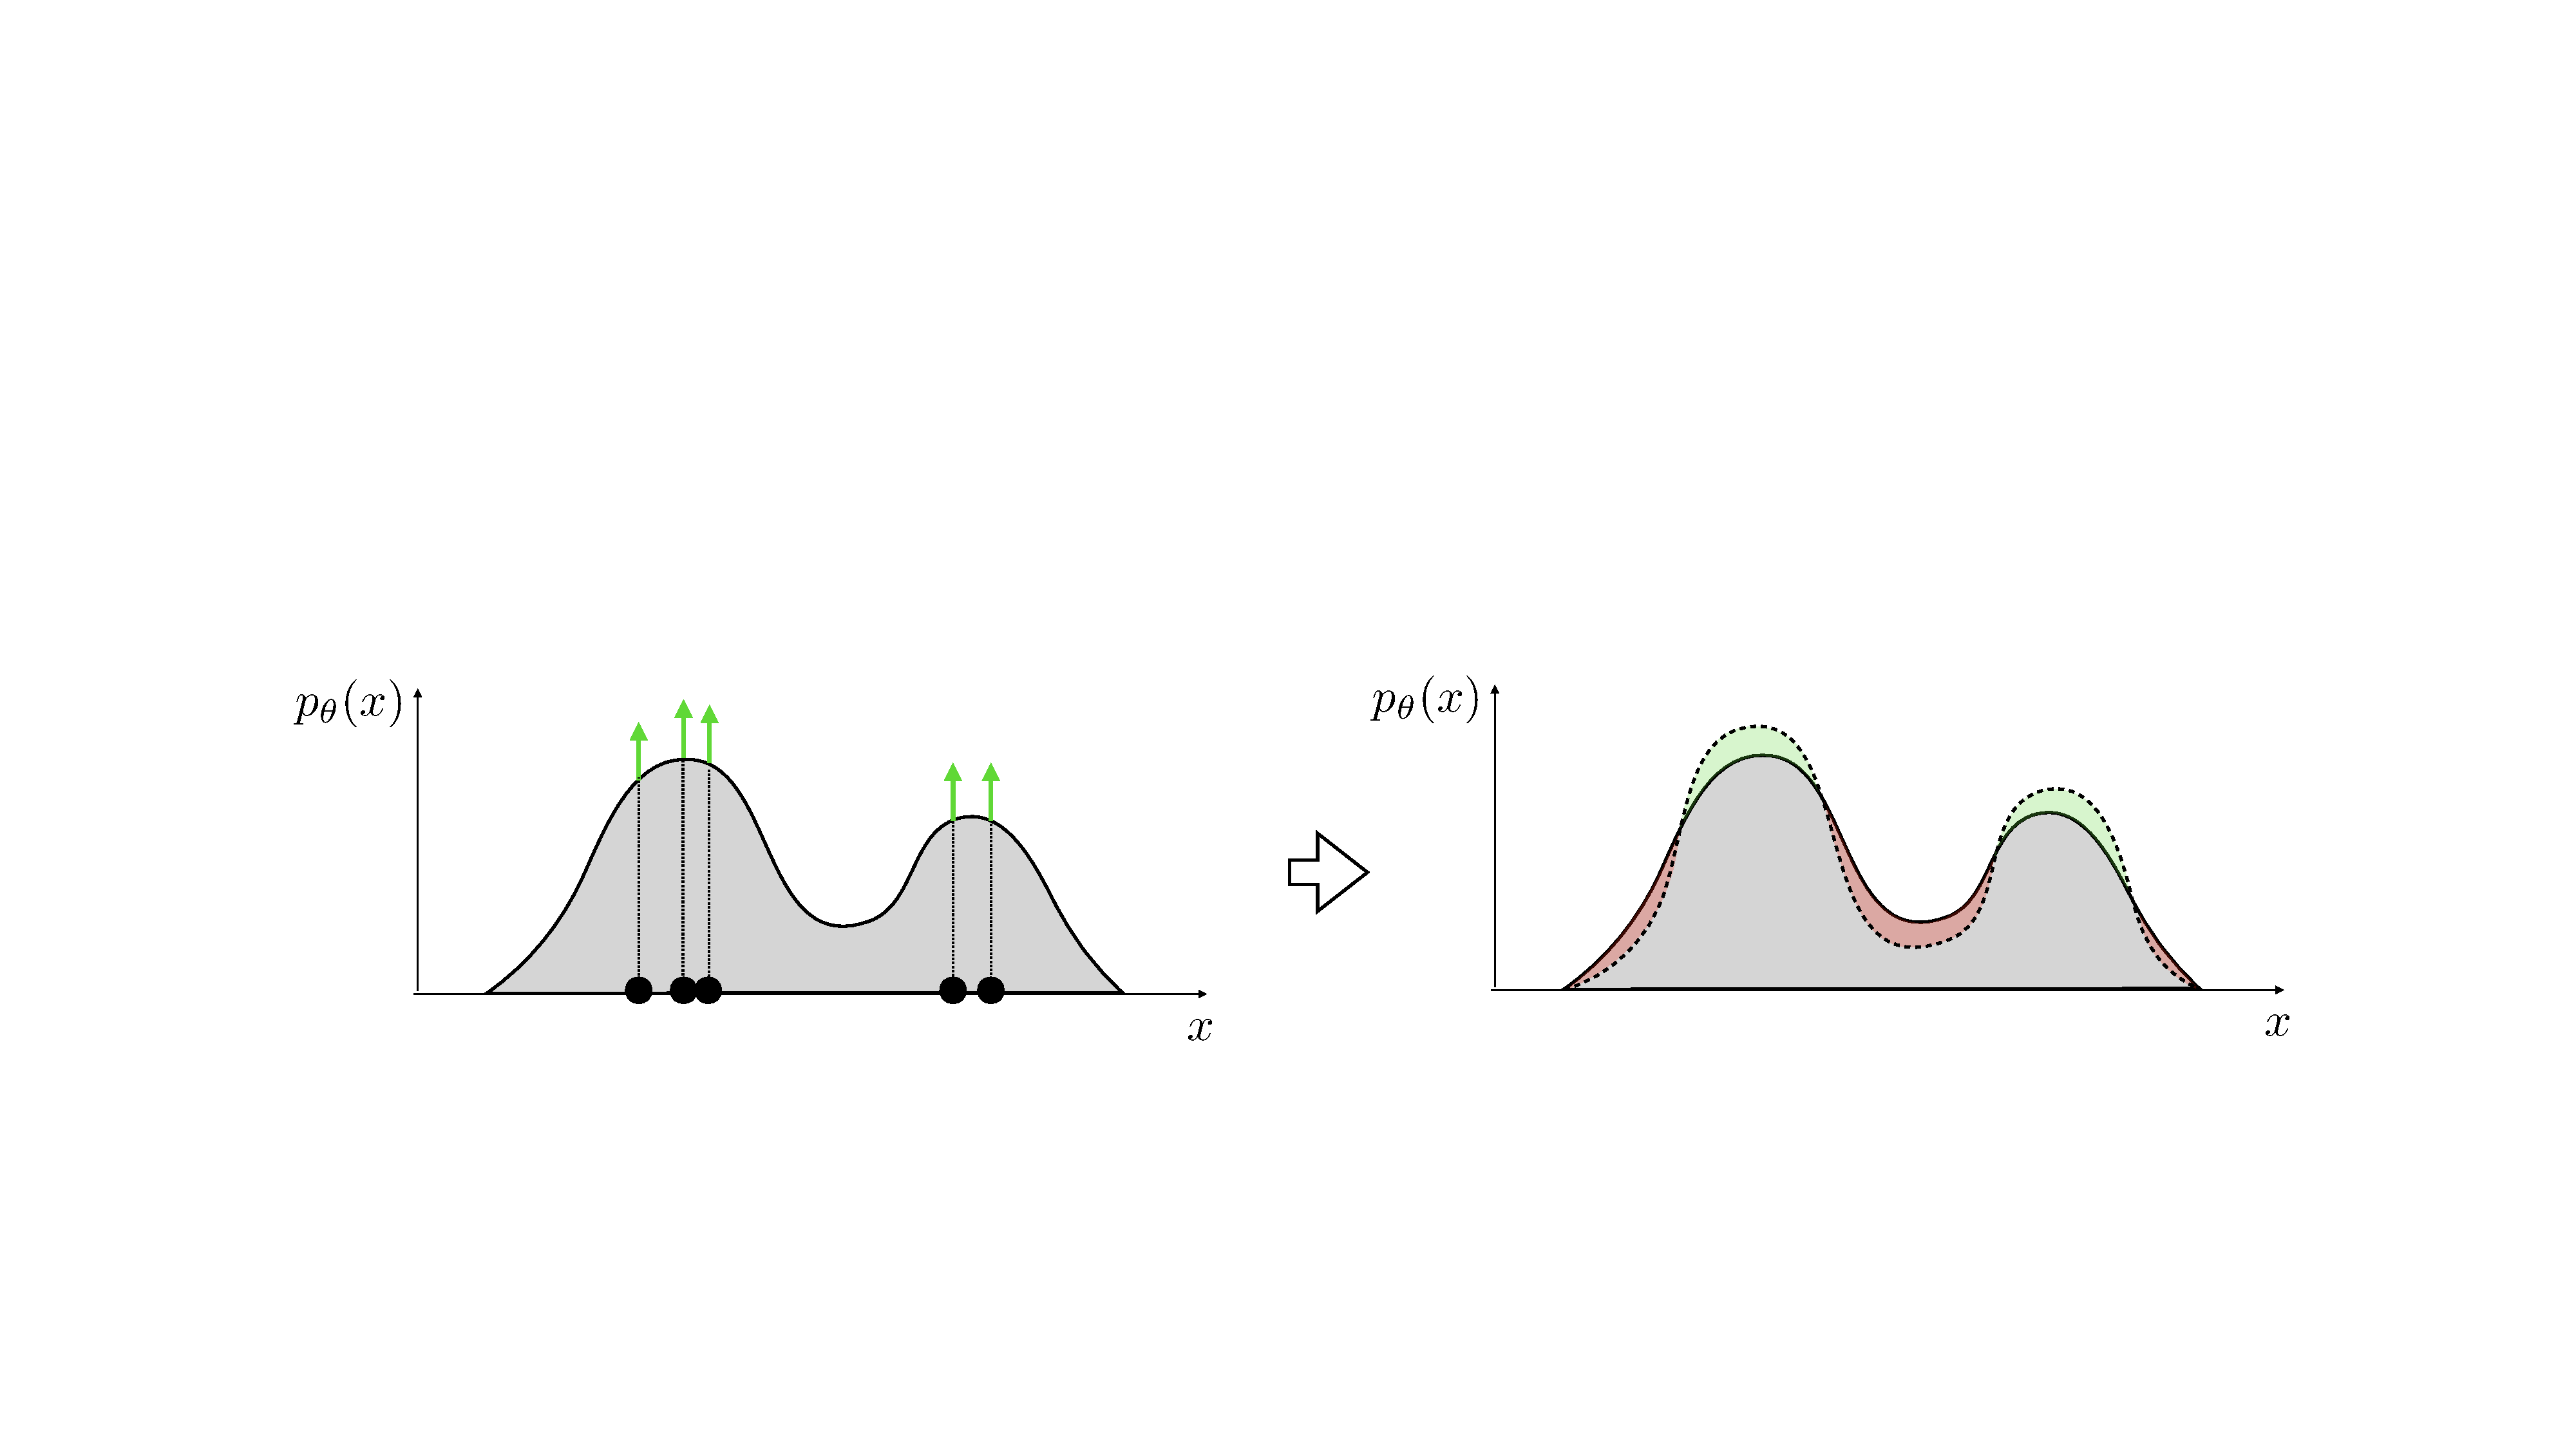
\includegraphics[width=1.0\linewidth]{./figures/generative_models/max_likelihood_density.pdf}
    }
    \caption{Fitting a max likelihood density model to data. The gray region holds a constant amount of mass; think of it as piles of dirt. To increase the amount of dirt at the locations of the green arrows you must remove dirt from other regions, indicated in red.}
    \label{fig:generative_models:max_likelihood_density}
\end{figure}


Remember that a probability density function (pdf) is a function $p_{\theta}: \mathcal{X} \rightarrow [0,\infty)$ with $\int_{\mathbf{x}} p_{\theta}(\mathbf{x})d\mathbf{x} = 1$ (i.e. it's normalized). To learn a pdf, we will typically learn the parameters of a family of pdfs. For example, in \sect{\ref{sec:generative_models:gaussian_density_models}}, we will cover learning the parameters of the Gaussian family of pdfs. All members of such a the family are normalized nonnegative functions; this way we do not need to add an explicit constraint that the learned function have these properties, we are simply searching over a space of functions \textit{all of which} have these properties. This means that whenever we push up density over datapoints, we are forced to sacrifice density over other regions, so implicitly we are removing density from places where there is no data, as indicated by the red regions in \fig{\ref{fig:generative_models:max_likelihood_density}}.

In the next section we will see an alternative approach where the parametric family we search over need not be normalized.

\section{Energy-Based Models}
\index{Energy-based models}
Density models constrain the learned function to be normalized, that is, $\int_{\mathbf{x}} p_{\theta}(\mathbf{x})d\mathbf{x} = 1$. This constraint is often hard to realize. One approach is to learn an unnormalized function $E_{\theta}$, then convert it to the normalized density $p_{\theta} = \frac{e^{-E_{\theta}}}{Z(\theta)}$, where $Z(\theta) = \int_{\mathbf{x}} e^{-E_{\theta}(\mathbf{x})}d\mathbf{x}$ is the normalizing constant. The $Z(\theta)$ can be very expensive to compute and often can only be approximated.\marginnote{The parametric form $\frac{e^{-E_{\theta}}}{Z(\theta)}$is sometimes referred to as a \textbf{Boltzmann} or \textbf{Gibbs distribution}.}[-1.8cm]\marginnote{Notice that $Z$ is a function of model parameters $\theta$ but not of datapoint $\mathbf{x}$, since we integrate over all possible data values.}[0.4cm]

\marginnote{Note that low energy $\Rightarrow$ high probability. So we minimize energy to maximize probability.}[3.6cm]

\textbf{Energy-based models} (\textbf{EBM}s) address this by simply skipping the step where we normalize the density, and letting the output of the learner just be $E_\theta$. Even though it is not a true probability density, $E_{\theta}$ can still be used for many of the applications we would want a density for. This is because we can compare \textit{relative probabilities} with $E_\theta$: %Both probability ratios and probability differences can be computed via basic functions of $E_{\theta}$.
% Probability ratio:
\begin{align}
    \frac{p_\theta(\mathbf{x}_1)}{p_\theta(\mathbf{x}_2)} = \frac{e^{-E_\theta(\mathbf{x}_1)}/Z(\theta)}{e^{-E_\theta(\mathbf{x}_2)}/Z(\theta)}
    = \frac{e^{-E_\theta(\mathbf{x}_1)}}{e^{-E_\theta(\mathbf{x}_2)}}
\end{align}
% \begin{align}
%     E_\theta(\mathbf{x}_1) - E_\theta(\mathbf{x}_2) &= \log e^{-E_\theta(\mathbf{x}_2) - -E_\theta(\mathbf{x}_1)}\\
%     &= \log \frac{e^{-E_\theta(\mathbf{x}_2)}}{e^{-E_\theta(\mathbf{x}_1)}}\\
%     &= \log \frac{e^{-E_\theta(\mathbf{x}_2)}/Z}{e^{-E_\theta(\mathbf{x}_1)}/Z}\\
%     &= \log \frac{p_\theta(\mathbf{x}_2)}{p_\theta(\mathbf{x}_1)}
% \end{align}

%Probability difference:
% \begin{align}
%     p_\theta(\mathbf{x}_1) - p_\theta(\mathbf{x}_2) &= \frac{e^{-E_\theta(\mathbf{x}_1)}}{Z} - \frac{e^{-E_\theta(\mathbf{x}_2)}}{Z}\\
%     &= \frac{e^{-E_\theta(\mathbf{x}_1)} - e^{-E_\theta(\mathbf{x}_2)}}{Z}\\
%     &= \frac{e^{-E_\theta(\mathbf{x}_1) / -E_\theta(\mathbf{x}_2)}}{Z}\\
%     &\propto e^{-E_\theta(\mathbf{x}_1) / -E_\theta(\mathbf{x}_2)}
% \end{align}

% Probability gradient:
% \begin{align}
%     \nabla_{\mathbf{x}} p(\mathbf{x}) = \nabla_{\mathbf{x}} e^{-E_\theta(\mathbf{x})}/Z \propto \nabla_{\mathbf{x}} e^{-E_\theta(\mathbf{x})}
% \end{align}


%since $\frac{E_\theta(\mathbf{x}_1)}{E_\theta(\mathbf{x}_2)} = \frac{p_\theta(\mathbf{x}_1)}{p_\theta(\mathbf{x}_2)}$, and \textit{probability differences} since $E_\theta(\mathbf{x}_1) - E_\theta(\mathbf{x}_2) = p_\theta(\mathbf{x}_1) - p_\theta(\mathbf{x}_2)$.
Knowing relative probabilities is all that is required for sampling (via MCMC), for outlier detection (the relatively lowest probability datapoint in a set of datapoints is the outlier), and even for optimizing over a space of of data to find the datapoint that is max probability (because $\argmax_{\mathbf{x} \in \mathcal{X}} p_{\theta}(\mathbf{x}) = \argmax_{\mathbf{x} \in \mathcal{X}} -E_{\theta}(\mathbf{x})$). To solve such a maximization problem, we might want to find the gradient of the log probability density with respect to $\mathbf{x}$; it turns out this gradient is identical to the gradient of $-E_{\theta}$ with respect to $\mathbf{x}$!
\begin{align}
    \nabla_{\mathbf{x}} \log p_{\theta}(\mathbf{x}) &= \nabla_{\mathbf{x}} \log \frac{e^{-E_{\theta}(\mathbf{x})}}{Z(\theta)}\\
    &= -\nabla_{\mathbf{x}} E_{\theta}(\mathbf{x}) - \nabla_{\mathbf{x}} \log Z(\theta)\\
    &= -\nabla_{\mathbf{x}} E_{\theta}(\mathbf{x})
\end{align}
In sum, energy functions can do most of what probability densities can do, except that they do not give normalized probabilities. Therefore, they are insufficient for applications where communicating probabilities is important for either interpretability or for interfacing with downstream systems that require knowing true probabilities.\marginnote{A case where a density model might be preferable over an energy model is a medical imaging system that needs to communicate to doctors the likelihood that a patient has cancer.}[-0.4cm]
%So it looks like energy functions are really all we need. However, there are other cases where knowing the normalized probability is still important. One such case might be in medical imaging, where we might prefer a density that tells us ``this blob in the scan is 90\% likely to be a tumor
%Another useful property of $E_{\theta}$ is that certain gradients of the probability density $p_{\theta}$ can be be computed or approximated given $E_{\theta}$.

\subsection{Learning Energy-Based Models}
Learning the parameters of an energy-based model is a bit different than learning the parameters of a density model. In a density model, we simply increase the probability mass over observed datapoints, and because the density is a normalized function, this implicitly pushes down the density assigned to regions where there is no observed data. Since energy functions are not normalized, we need to add an explicit negative term to push up energy where there are no datapoints, in addition to the positive term of pushing down energy where the data is observed. One way to do so is called \index{Contrastive divergence}\textbf{contrastive divergence}~\cite{hinton2002training}. On each iteration of optimization, this method modifies the energy function to decrease the energy assigned to samples from the data (positive term) and to increase the energy assigned to samples from the model (i.e., samples from the energy function itself; negative term), as shown in \fig{\ref{fig:generative_models:contrastive_divergence}}:
\begin{figure}[h]
    \centerline{
    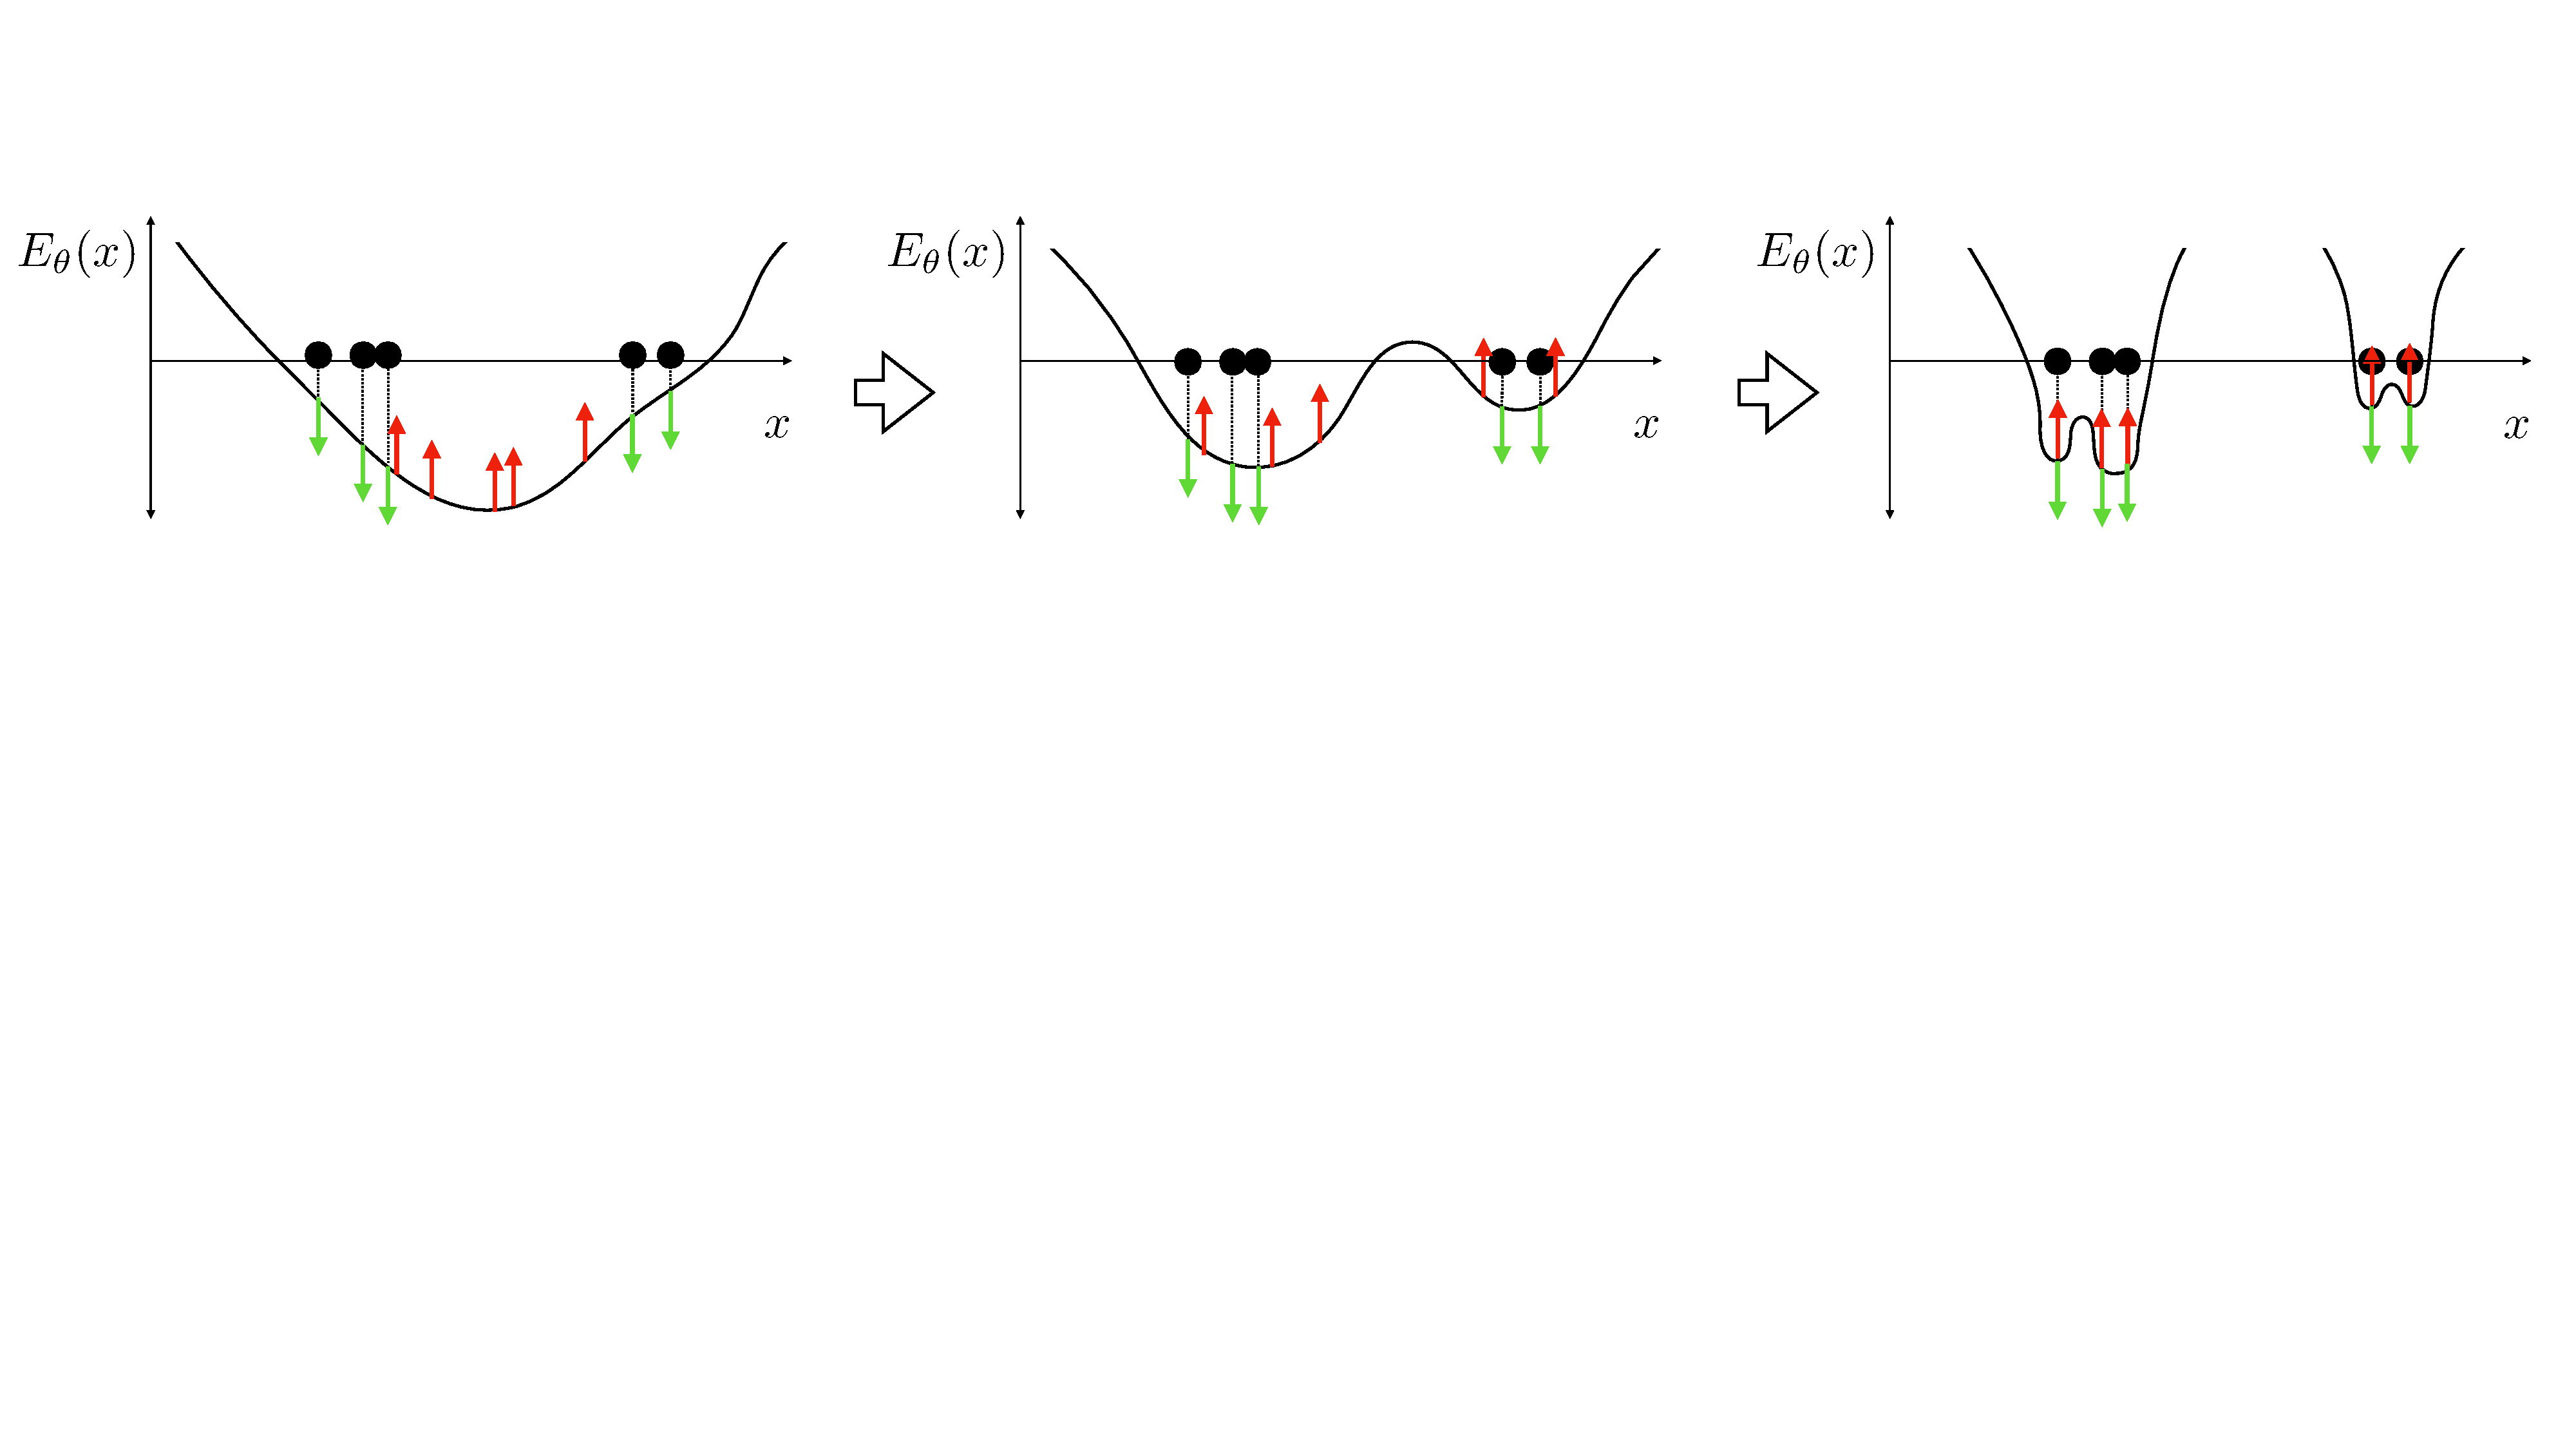
\includegraphics[width=1.0\linewidth]{./figures/generative_models/contrastive_divergence.pdf}
    }
    \caption{Fitting a max likelihood energy function to data, using contrastive divergence~\cite{hinton2002training}.}
    \label{fig:generative_models:contrastive_divergence}
\end{figure}

Once the energy function perfectly adheres to the data, samples from the model are identical to samples from the data and the positive and negative terms cancel out. This should make intuitive sense because we don't want the energy function to change once we have perfectly fit the data. It turns out that mathematically this procedure is an approximation to the gradient of the log likelihood function. Defining $p_{\theta} = \frac{e^{-E_{\theta}}}{Z(\theta)}$, start by decomposing the gradient of the log likelihood into two terms, which, as we will see, will end up playing the role of positive and negative terms:
\begin{align}
    \nabla_{\theta} \mathbb{E}_{\mathbf{x} \sim p_{\texttt{data}}}[\log p_{\theta}(\mathbf{x})] &= \nabla_{\theta} \mathbb{E}_{\mathbf{x} \sim p_{\texttt{data}}}[\log \frac{e^{-E_{\theta}(\mathbf{x})}}{Z(\theta)}]\\
    &= -\mathbb{E}_{\mathbf{x} \sim p_{\texttt{data}}}[\nabla_{\theta} E_{\theta}(\mathbf{x})] - \nabla_{\theta} \log Z(\theta)\label{eqn:generative_models:cd}
\end{align}
The first term is the positive term gradient, which tries to modify parameters to decrease the energy placed on data samples. The second term is the negative term gradient; here it appears as an intractable integral, so our strategy is to rewrite it as an expectation, which can be approximated via sampling:
\marginnote{In \eqn{\ref{eqn:generative_models:grad_log_identity}} we use a very useful identity from the chain rule of calculus, which appears often in machine learning: $\nabla_{x} \log f(x) = \frac{1}{f(x)} \nabla_{x} f(x)$}[1cm]
\begin{align}
    \nabla_{\theta} \log Z(\theta) &= \frac{1}{Z(\theta)}\nabla_{\theta}Z(\theta) \label{eqn:generative_models:grad_log_identity} \\
    &= \frac{1}{Z(\theta)} \nabla_{\theta} \int_x e^{-E_{\theta}(\mathbf{x})}d\mathbf{x} &&\quad\quad \triangleleft \quad \text{definition of $Z$}\\
    &= \frac{1}{Z(\theta)} \int_x \nabla_{\theta} e^{-E_{\theta}(\mathbf{x})}d\mathbf{x} &&\quad\quad \triangleleft \quad \text{exchange sum and grad}\\
    &= \frac{1}{Z(\theta)} -\int_x e^{-E_{\theta}(\mathbf{x})} \nabla_{\theta} E_{\theta}(\mathbf{x})d\mathbf{x}\\
    &= -\int_x \frac{e^{-E_{\theta}(\mathbf{x})}}{Z(\theta)} \nabla_{\theta} E_{\theta}(\mathbf{x})d\mathbf{x}\\
    &= -\int_x p_{\theta}(\mathbf{x}) \nabla_{\theta} E_{\theta}(\mathbf{x})d\mathbf{x} &&\quad\quad \triangleleft \quad \text{definition of $p_{\theta}$}\\
    &= -\mathbb{E}_{\mathbf{x} \sim p_{\theta}}[\nabla_{\theta} E_{\theta}(\mathbf{x})] &&\quad\quad \triangleleft \quad \text{definition of expectation}\label{eqn:generative_models:cd_neg}
\end{align}
Plugging \eqn{\ref{eqn:generative_models:cd_neg}} back into \eqn{\ref{eqn:generative_models:cd}}, we arrive at:
\begin{align}
    \nabla_{\theta} \mathbb{E}_{\mathbf{x} \sim p_{\texttt{data}}}[\log p_{\theta}(\mathbf{x})] &= -\mathbb{E}_{\mathbf{x} \sim p_{\texttt{data}}}[\nabla_{\theta}E_{\theta(\mathbf{x})}] + \mathbb{E}_{\mathbf{x} \sim p_{\theta}}[\nabla_{\theta} E_{\theta}(\mathbf{x})]
\end{align}
Both expectations can be approximated via sampling: defining $\mathbf{x}^{(i)} \sim p_{\texttt{data}}$ and $\hat{\mathbf{x}}^{(i)} \sim p_{\theta}$, and taking $N$ such samples, we have
\begin{align}
    -\mathbb{E}_{\mathbf{x} \sim p_{\texttt{data}}}[\nabla_{\theta}E_{\theta(\mathbf{x})}] + \mathbb{E}_{\mathbf{x} \sim p_{\theta}}[\nabla_{\theta} E_{\theta}(\mathbf{x})] &\approx -\frac{1}{N} \sum_{i=1}^N \nabla_{\theta}E_{\theta}(\mathbf{x}^{(i)}) + \frac{1}{N} \sum_{i=1}^N \nabla_{\theta}E_{\theta}(\hat{\mathbf{x}}^{(i)})\\
    &= \frac{1}{N} \nabla_{\theta} \sum_{i=1}^N (-E_{\theta}(\mathbf{x}^{(i)}) + E_{\theta}(\hat{\mathbf{x}}^{(i)}))
\end{align}
The last line should make clear the intuition: we establish a contrast between data samples and current model samples, then update the model to decrease this contrast, bringing the model closer to the data. Once $\mathbf{x}^{(i)}$ and $\hat{\mathbf{x}}^{(i)}$ are identically distributed, this gradient will be zero (in expectation); we have perfectly fit the data and no further updates should be taken.

Under our formalization of a learning problem as an objective, hypothesis space, and optimizer, contrastive divergence is an \textit{optimizer}; it's an optimizer specifically built for max likelihood objectives over energy functions. Contrastive divergence tells us how to approximate the gradient of the likelihood function, which can then be plugged into any gradient descent method.

%Use the gradient, then score function makes it simple. $\nabla_{\theta} \mathbb{E}_{x \sim p_{\theta}}[f(x)] = \mathbb{E}_{x \sim p_{\theta}}[f(x) \nabla_{\theta} \log p_{\theta}(x)]$ \marginnote{A useful identity to remember: $\nabla_{x} \log f(x) = \frac{1}{f(x)} \nabla_{x} f(x)$}

%The positive term in learning an energy function can be max likelihood, just like in learning a density function. The negative term can take on a variety of different forms. One option is to make the negative term an estimate of the normalizing constant $Z = \mathbb{E}_{\mathbf{x} \sim E_{\theta}}[e^{-E_{\theta}(\mathbf{x})}]$, which can be approximated via sampling. One approach that does this is called \textbf{contrastive divergence}~\cite{hinton2002training}. This is a max likelihood method, which estimates the gradient of the data likelihood, under the normalized energy as:
%\begin{align}
%    \nabla_{\theta}\mathbb{E}_{\mathbf{x} \sim p_{\texttt{data}}}[\log \frac{e^{-E_{\theta}(\mathbf{x})}}{Z(\theta)}]\\
%    &= \mathbb{E}_{\mathbf{x} \sim p_{\texttt{data}}}[\nabla_{\theta}[-E_{\theta}(\mathbf{x})] - \nabla_{\theta} \log Z(\theta)\\
%    &= \mathbb{E}_{\mathbf{x} \sim p_{\texttt{data}}}[\nabla_{\theta}[-E_{\theta}(\mathbf{x})] - \log \mathbb{E}_{\mathbf{x} \sim E_{\theta}}[e^{-E_{\theta}(\mathbf{x})}]
%\end{align}
%where, in the final line, the first expectation can be approximated by sampling from the data and the second expectation can be approximated by sampling from the model.
%It turns out to also be sufficient to set the negative distribution to be any arbitrary distribution that has nonzero support wherever the positive distribution has nonzero support, using the framework of \textbf{noise contrastive estimmation}~\cite{gutmann2010noise} (but some choices of negative distribution will lead to lower-variance estimates than others). The general theme with fitting energy functions is to build an energy that \textit{contrasts} between ``positive" samples from the data distribution and ``negative" samples from some other distribution.


%, for finding a datapoint $\mathbf{x}$ with maximum probability, and so on. One important function that relies on relative probabilities is the gradient of a log density function w.r.t. $\mathbf{x}$, i.e. $\nabla_{\mathbf{x}} \log p_{\theta}(\mathbf{x})$.
%For example, suppose we want to find an image $\mathbf{x}$ that has maximum probability under $p_{\theta}$. Then we may descent the gradient of a log density function w.r.t. $\mathbf{x}$, i.e. $\nabla_{\mathbf{x}} \log p_{\theta}(\mathbf{x})$, and we can do this via $E_{\theta}$:
% \begin{align}
%     \nabla_{\mathbf{x}} \log p_{\theta}(\mathbf{x}) &= \nabla_{\mathbf{x}} \log \frac{e^{E_{\theta}(\mathbf{x})}}{Z}\\
%     &= \nabla_{\theta} E_{\theta}(\mathbf{x}) - \nabla_{\mathbf{x}} \log Z\\
%     &= \nabla_{\theta} E_{\theta}(\mathbf{x})
% \end{align}
%
%Often we wish to take gradients of the log probability of the data w.r.t. to the parameters, $\theta$, of the density function. This calculation can also be done in terms of $E_{\theta}$ but does require an integral. Fortunately, the integral has the form of an expectation over samples from the model, and can therefore be approximated via sampling, which is how \textbf{contrastive divergence} learning algorithms work:

% \begin{align}
%     \nabla_{\theta} \log p_{\theta}(\mathbf{x}) &= \nabla_{\theta} \log \frac{e^{E_{\theta}(\mathbf{x})}}{Z}\\
%     &= \nabla_{\theta} E_{\theta}(\mathbf{x}) - \nabla_{\theta} \log Z\\
%     &= \nabla_{\theta} E_{\theta}(\mathbf{x}) - \nabla_{\theta} \log \mathbb{E}[e^{-E_{\theta}(\mathbf{x}}]\\
%     &= \nabla_{\theta} E_{\theta}(\mathbf{x}) - \nabla_{\theta} \log \int_{\mathbf{x}} e^{-E_{\theta}(\mathbf{x}} d\mathbf{x}\\
% \end{align}

%\section{A Tour of Popular Generative Models}
\subsection{Comparing Different Kinds of Generative Models}
Some generative models give density or energy functions, others give generator functions, and still others give both. We can summarize all these kinds of models with the following learning diagram: %The kinds of {\bf deep generative models} that are popular these days, have the following form:
\begin{center}
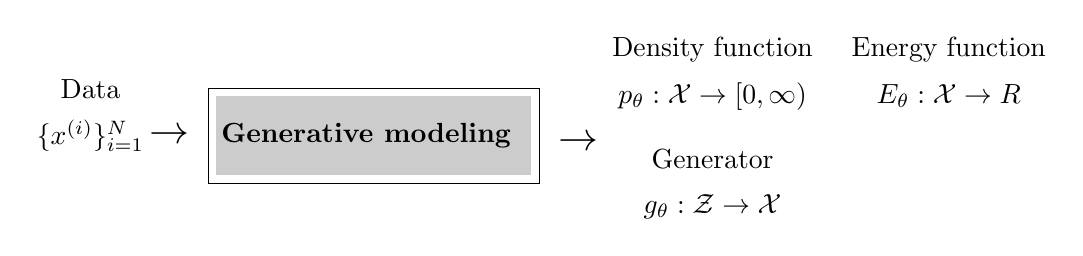
\begin{tikzpicture}
    \draw (0,1.2) rectangle (4.2,2.4); % outer box
    \fill[black!20] (0.1,1.3) rectangle (4.1,2.3); % gray box
    \node[] at (2.0,1.8) {{\bf Generative modeling}};
    \node[] at (-1.5,2.4) {Data};
    \node[] at (-1.5,1.8) {$\{x^{(i)}\}_{i=1}^N$};
    \node[] at (-0.5,1.8) {{\Large  $ \rightarrow$}};
    \node[] at (6.4,2.9) {Density function};
    \node[] at (6.4,2.3) {$p_{\theta}: \mathcal{X} \rightarrow [0,\infty)$};
    \node[] at (9.4,2.9) {Energy function};
    \node[] at (9.4,2.3) {$E_{\theta}: \mathcal{X} \rightarrow \mathbb{R}$};
    \node[] at (6.4,1.5) {Generator};
    \node[] at (6.4,0.9) {$g_{\theta}: \mathcal{Z} \rightarrow \mathcal{X}$};
    \node[] at (4.7,1.7) {{\Large $ \rightarrow$}};
\end{tikzpicture}
\end{center}

Each of these families of model has its own advantages and disadvantages. Generators have latent variables $\mathbf{z}$ that control the properties of the generated image. Changing these variables can change the generated image in meaningful ways; we will explore this idea in greater detail in the next chapter. In contrast, density and energy models do not have latent variables that directly control generated samples.\marginnote{While density/energy functions do not have latent variables, when we draw samples from them we use a \textit{sampling algorithm} that does, necessarily, depend on stochastic factors, which can be considered latent variables of the sampler.}[-0.4cm] 
Conversely, an advantage of density/energy functions is that they provide scores related to the likelihood of data. These scores (densities or energies) can be used to detect anomalies and unusual events, or can be optimized to synthesize higher quality data.

%It's worth noting a special property of generative models that learn a generator $g_{\theta}$. The ``noise" $\mathbf{z}$ input to the generator acts as \textbf{latent variables} that control the properties of the generated image. Changing these variables can change the generated image in meaningful ways -- we will explore this idea in greater detail in the next two chapters. In contrast, density and energy models do not have latent variables that directly control generated samples.\marginnote{While density/energy functions do not have latent variables, when we draw samples from them we use a \textit{sampling algorithm} that does, necessarily, depend on stochastic factors, which can be considered latent variable of the sampler.}[-1.8cm]

Some of the generative models we will describe in this chapter and the next are categorized along these dimensions in \tab{\ref{tab:generative_models:types_of_gen_model}}. Note that this is a rough categorization, meant to reflect the most straightforward usage of these models. With additional effort some of the \xmark's can be converted to \checkmark's; for example, one can do additional inference to sample from a density model, or one can extract a lower-bound estimate of density from a variational autoencoder (VAE) or diffusion model.
% \begin{table}[h]
%     \centering
%     \begin{tabular}{c|c|c|c}
%         Method & Explicit latents? & Explicit density? & Explicit generator? \\
%         \hline
%         Normalizing flow & \checkmark (high-dimensional) & \checkmark & \checkmark \\
%         VAE & \checkmark & & \checkmark \\
%         GAN & \checkmark & & \checkmark \\
%         Autoregressive models &  & \checkmark & \\
%         Energy-based models &  & \checkmark (unnormalized) & \\
%     \end{tabular}
%     \caption{Three desirable properties in a generative model. No method achieves all three (without caveats). VAEs and GANs are good at representation learning (i.e. at finding a low-dimensional latent space). Normalizing flows and autoregressive models are great if you want to estimate the likelihood of your data points (e.g., for anomaly detection). Energy-based models can be an especially efficient way to model an unnormalized density.}
%     \label{tab:generative_models:types_of_gen_model}
% \end{table}
\begin{table}[h]
    \caption{Three desirable properties in a generative model. No method achieves all three (without caveats). VAEs (see \chap{\ref{chapter:generative_modeling_and_representation_learning}}) and GANs are good at representation learning (i.e., at finding a low-dimensional latent space). Autoregressive models are great if you want to estimate the likelihood of your data points. Energy-based models can be an especially efficient way to model an unnormalized density.}
    %\marginnote{{\bf Table \ref{tab:generative_models:types_of_gen_model}}: Three desirable properties in a generative model. No method achieves all three (without caveats). VAEs (see \chap{\ref{chapter:generative_modeling_and_representation_learning}}) and GANs are good at representation learning (i.e., at finding a low-dimensional latent space). Autoregressive models are great if you want to estimate the likelihood of your data points. Energy-based models can be an especially efficient way to model an unnormalized density.}
    \label{tab:generative_models:types_of_gen_model} 
    \centering
    \begin{tabular}{c|c|c|c}
        Method & Latents? & Density/Energy? & Generator? \\
        \hline
        Energy-based models & \xmark & \checkmark (energy only) & \xmark \\
        Gaussian & \xmark & \checkmark & \xmark \\
        Autoregressive models & \xmark & \checkmark & \checkmark (slow) \\
        Diffusion models & \checkmark (high-dimensional) & \xmark & \checkmark (slow) \\
        GANs & \checkmark & \xmark & \checkmark \\
        VAEs & \checkmark & \xmark & \checkmark
    \end{tabular}
\end{table}

Generative models can also be distinguished according to their objectives, hypothesis spaces, and optimization algorithms. Some classes of model, such as autoregressive models, refer to just a particular kind of hypothesis space, whereas other classes of model, such as VAEs, are much more specific in referring to the conjunction of an objective, a general family of hypothesis spaces, and a particular optimization algorithm.

In the next sections, and in the next chapter, we will dive into the details of exactly how each of these models works.


% \begin{figure}[h]
%     \centering
%     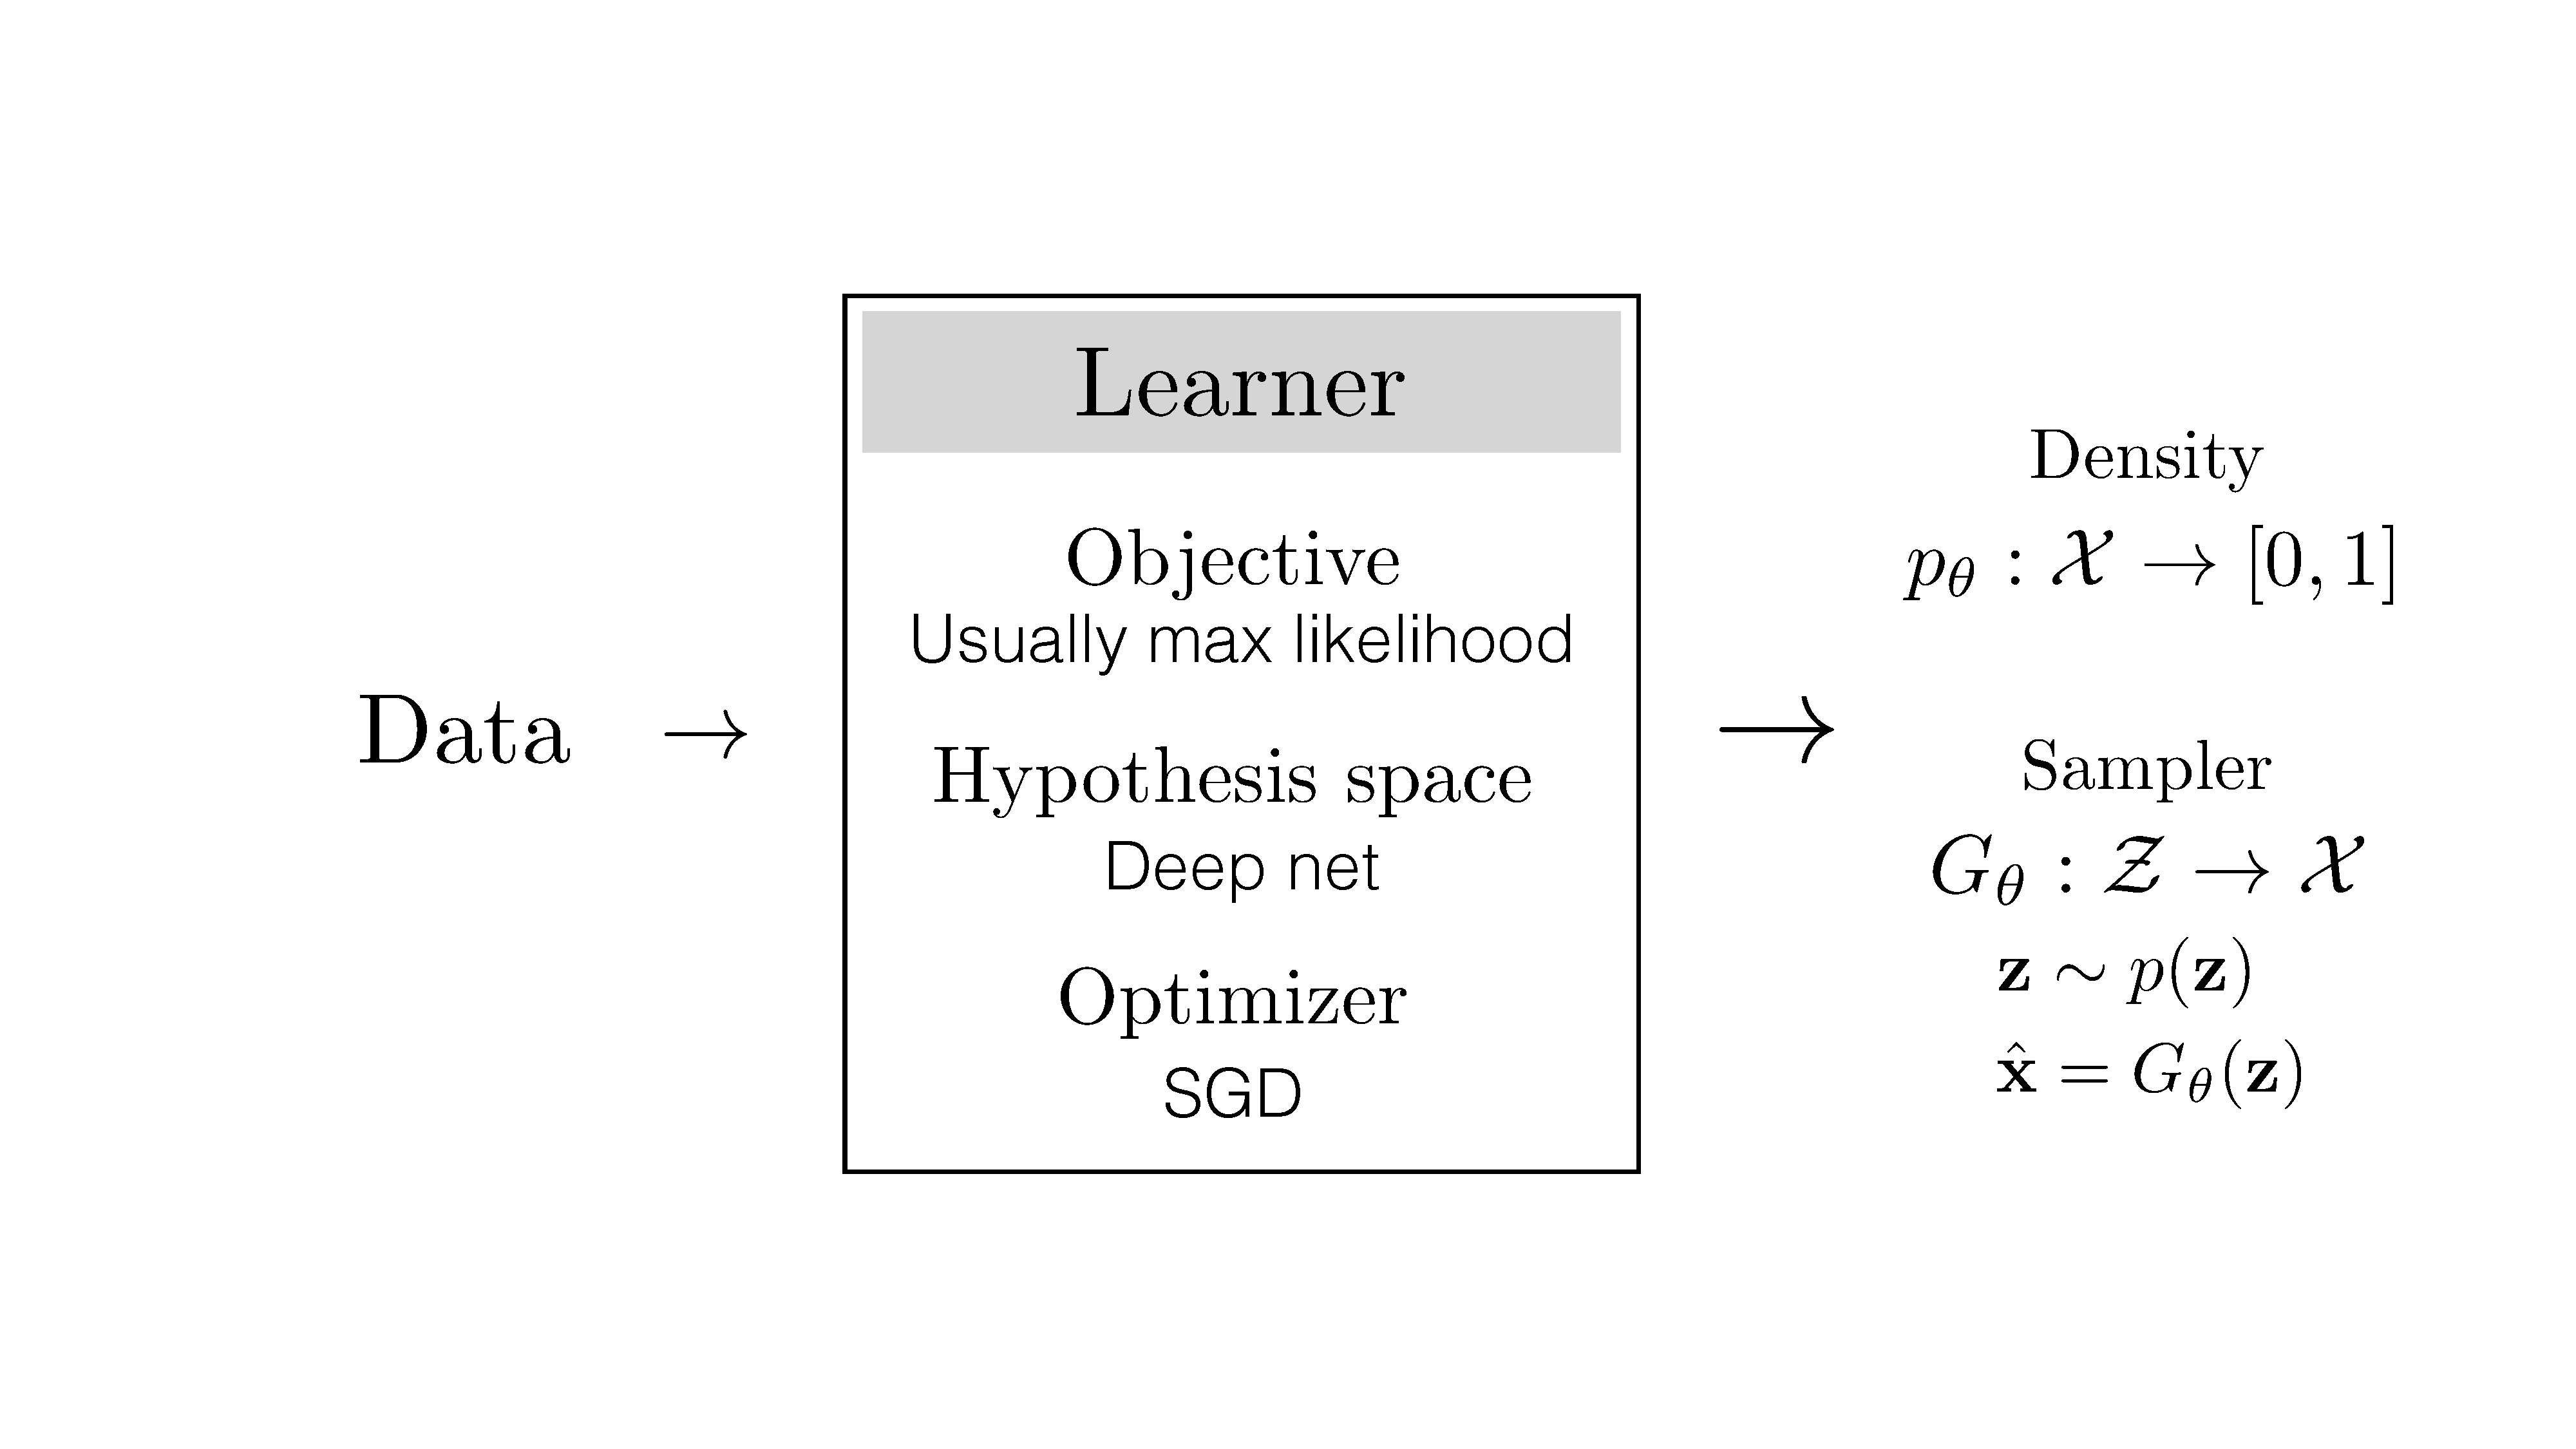
\includegraphics[width=0.8\linewidth]{./figures/generative_models/deep_generative_model_formalism.pdf}
%     \label{fig:deep_generative_model_formalism}
% \end{figure}

\section{Gaussian Density Models}\label{sec:generative_models:gaussian_density_models}

One of the simplest and most useful density models is the Gaussian distribution, which in one dimension (1D) is:
\begin{align}
    p_{\theta}(x) = \frac{1}{Z}e^{-(x-\theta_1)^2/(2\theta_2)}
\end{align}
\marginnote{For 1D Gaussians $Z=\frac{1}{\sqrt{2\pi\theta_2}}$. We prefer to write it as $Z$ to emphasize its structural role as a normalization constant. Usually we will not be explicitly evaluating normalization constants, and will not require knowing their analytical form.}[-2.2cm]
This density has two parameters $\theta_1$ and $\theta_2$, which are the mean and variance of the distribution. The normalization constant $Z$ ensures that the function is normalized. This is the typical strategy in defining density models: create a parameterized family of functions such that any function in the family is normalized. Given such a family, we search over the parameters to optimize a generative modeling objective.

For density models, the most common objective is max likelihood:
\begin{align}
     \mathbb{E}_{x \sim p_{\texttt{data}}}[\log p_{\theta}(x)] \approx \frac{1}{N} \sum_{i=1}^N \log p_{\theta}(x^{(i)})
\end{align}
For a 1D Gaussian, this has a simple form:
\begin{align}
     \frac{1}{N} \sum_{i=1}^N \log \frac{1}{Z}e^{-(x^{(i)}-\theta_1)^2/(2\theta_2)} = -\log(Z) + \frac{1}{N}\sum_{i=1}^N (x^{(i)}-\theta_1)^2/(2\theta_2)
\end{align}
Optimizing with respect to $\theta_1$ and $\theta_2$ could be done via gradient descent or random search, but in this case there is also an analytical solution we can find by setting the gradient to be zero. For $\theta_1^*$ we have:
\begin{align}
    \frac{\partial \big(-\log Z + \frac{1}{N}\sum_{i=1}^N (x^{(i)}-\theta_1^*)^2/(2\theta_2^*)\big)}{\partial \theta_1^*} = 0\\
    %-\sum_{i=1}^N \frac{\partial  (x^{(i)}-\theta_1^*)^2/(2\theta_2^*)}{\partial \theta_1^*} = 0\\
    \frac{1}{N}\sum_{i=1}^N 2(x^{(i)}-\theta_1^*)/(2\theta_2^*) = 0\\
    \sum_{i=1}^N x^{(i)} - \sum_{i=1}^N \theta_1^* = 0\\
    %\sum_{i=1}^N \theta_1^* = \sum_{i=1}^N x^{(i)}\\
    %N\theta_1^* = \sum_{i=1}^N x^{(i)}\\
    \theta_1^* = \frac{1}{N}\sum_{i=1}^N x^{(i)}
\end{align}
For $\theta_2^*$ we need to note that $Z$ depends on  $\theta_2^*$ and in particular notice that $\frac{\partial (-\log Z)}{\partial \theta_2^*} = \frac{1}{2\theta_2^*}$:
\begin{align}
    \frac{\partial \big(-\log Z + \frac{1}{N}\sum_{i=1}^N (x^{(i)}-\theta_1^*)^2/(2\theta_2^*)\big)}{\partial \theta_2^*} = 0\\
    \frac{1}{2\theta_2^*} - \frac{1}{N}\sum_{i=1}^N 2(x^{(i)}-\theta_1^*)^2/(2\theta_2^*)^2 = 0\\
    2\theta_2^* - \frac{1}{N}\sum_{i=1}^N 2(x^{(i)}-\theta_1^*)^2 = 0\\
    \theta_2^* = \frac{1}{N}\sum_{i=1}^N (x^{(i)}-\theta_1^*)^2
\end{align}
% \begin{align}
%     \theta_1^* &= \argmin_{\theta_1} \mathbb{E}_{x \sim p_{\texttt{data}}}[-(x-\theta_1)^2/(2\theta_2)] = \mathbb{E}_{x \sim p_{\texttt{data}}}[x]\\
%     \theta_2^* &= \argmin_{\theta_2} \mathbb{E}_{x \sim p_{\texttt{data}}}[-(x-\theta_1)^2/(2\theta_2)] = \mathbb{E}_{x \sim p_{\texttt{data}}}[(x-\theta_1^*)^2]
% \end{align}
You might recognize the solutions for $\theta_1^*$ and $\theta_2^*$ as the empirical mean and variance of the data, respectively. This makes sense: we have just shown that to maximize the probability of the data under a Gaussian, we should set the mean and variance of the Gaussian to be the empirical mean and variance of the data.

This fully describes the learning problem, and solution, for a 1D Gaussian density model. We can put it all together in the learning diagram below:
\begin{center}
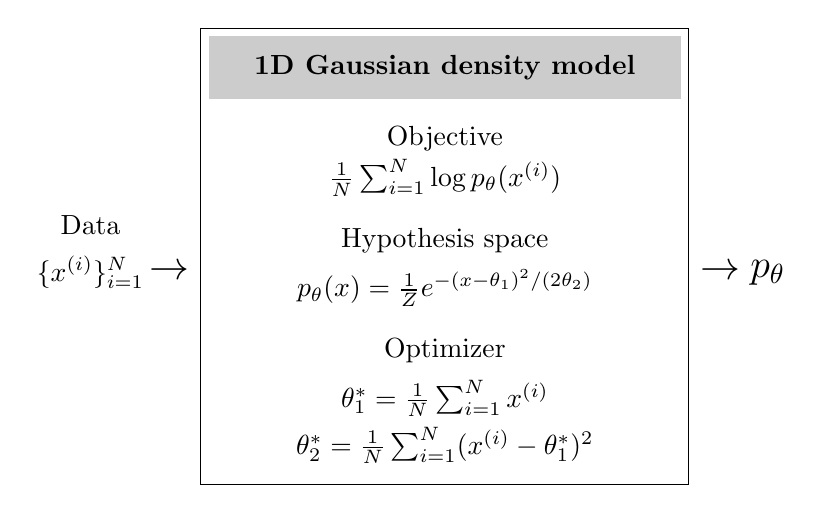
\begin{tikzpicture}
    \draw (0,-0.6) rectangle (6.2,5.2); % outer box
    \fill[black!20] (0.1,4.3) rectangle (6.1,5.1); % gray box
    \node[] at (3.1,4.7) {{\bf 1D Gaussian density model}};
    \node[] at (3.1,3.8) {Objective}; \node[] at (3.1,3.3) {$\frac{1}{N} \sum_{i=1}^N \log p_{\theta}(x^{(i)})$};
    \node[] at (3.1,2.5) {Hypothesis space}; \node[] at (3.1,1.9) {$p_{\theta}(x) = \frac{1}{Z}e^{-(x-\theta_1)^2/(2\theta_2)}$};
    \node[] at (3.1,1.1) {Optimizer}; \node[] at (3.1,0.5) {$\theta_1^* = \frac{1}{N}\sum_{i=1}^N x^{(i)}$}; \node[] at (3.1,-0.1) {$\theta_2^* = \frac{1}{N}\sum_{i=1}^N (x^{(i)}-\theta_1^*)^2$};
    \node[] at (-1.4,2.7) {Data};
    \node[] at (-1.4,2.1) {$\{x^{(i)}\}_{i=1}^N$};
    \node[] at (-0.4,2.1) {{\Large  $ \rightarrow$}};
    \node[] at (7.2,2.1) {{\Large $p_{\theta}$}};
    \node[] at (6.6,2.1) {{\Large  $ \rightarrow$}};
\label{fig:1d_gaussian_summmary}
\end{tikzpicture}
\end{center}
Gaussian density models are just about the simplest density models one can come up with. You may be wondering, do we actually use them for anything in computer vision, or are they just a toy example? The answer is that \textit{yes} we do use them—in fact, we use them all the time. For example, in least-squares regression, we are simply fitting a Gaussian density to the conditional probability $p(Y \given X)$. If we want a more complicated density, we may use a mixture of multiple Gaussian distributions, called a \textbf{Gaussian mixture model} (\textbf{GMM}), which we will encounter in the next chapter. It's useful to get comfortable with Gaussian fits because (1) they are a subcomponent of many more sophisticated models, and (2) they showcase all the key components of density modeling, with a clear objective, a parameterized hypothesis space, and an optimizer that finds the parameters that maximize the objective.

\section{Autoregressive Density Models}\label{sec:generative_models:autoregressive}
\index{Autogressive model}
A single Gaussian is a very limited model, and the real utility of Gaussians only shows up when they are part of a larger modeling framework. Next we will consider a recipe for building highly expressive models out of simple ones. There are many such recipes and the one we focus on here is called an \textbf{autoregressive model}.

The idea of an autoregressive model is to synthesize an image pixel by pixel. Each new pixel is decided on based on the sequence already generated. 
%We will start with a very simple and intuitive model, where we synthesize images by sampling pixels one by one. Each new pixel is decided on based on the sequence already generated. Such an approach is called an {\bf autoregressive model}. These are max likelihood models: they learn a distribution over pixels that maximizes the density assigned to observed pixels in the training data. 
You can think of this as a simple sequence prediction problem: given a sequence of observed pixels, predict the color of the next one. We use the same learned function $f_{\theta}$ to make each subsequent prediction. 

\Fig{\ref{fig:generative_models:autoregressive_prediction_schematic}} shows this setup. We predict each next pixel from the partial image already completed. The red bordered region is the \index{Autoregressive model!Context}\textbf{context} the prediction is based on. This context could be the entire image synthesized so far or it could be a smaller region, like shown here. The green bordered pixel is the one we are predicting given this context. In this example, we always predict the bottom-center pixel in the context window. After making our prediction, we decide what color pixel to add to the image based on that prediction; we may add the color predicted as most likely, or we might sample from the predicted distribution so that we get some randomness in our completion. Then, to predict the next missing pixel we slide the context over by one and repeat.

\begin{figure}[t]
    \centerline{
    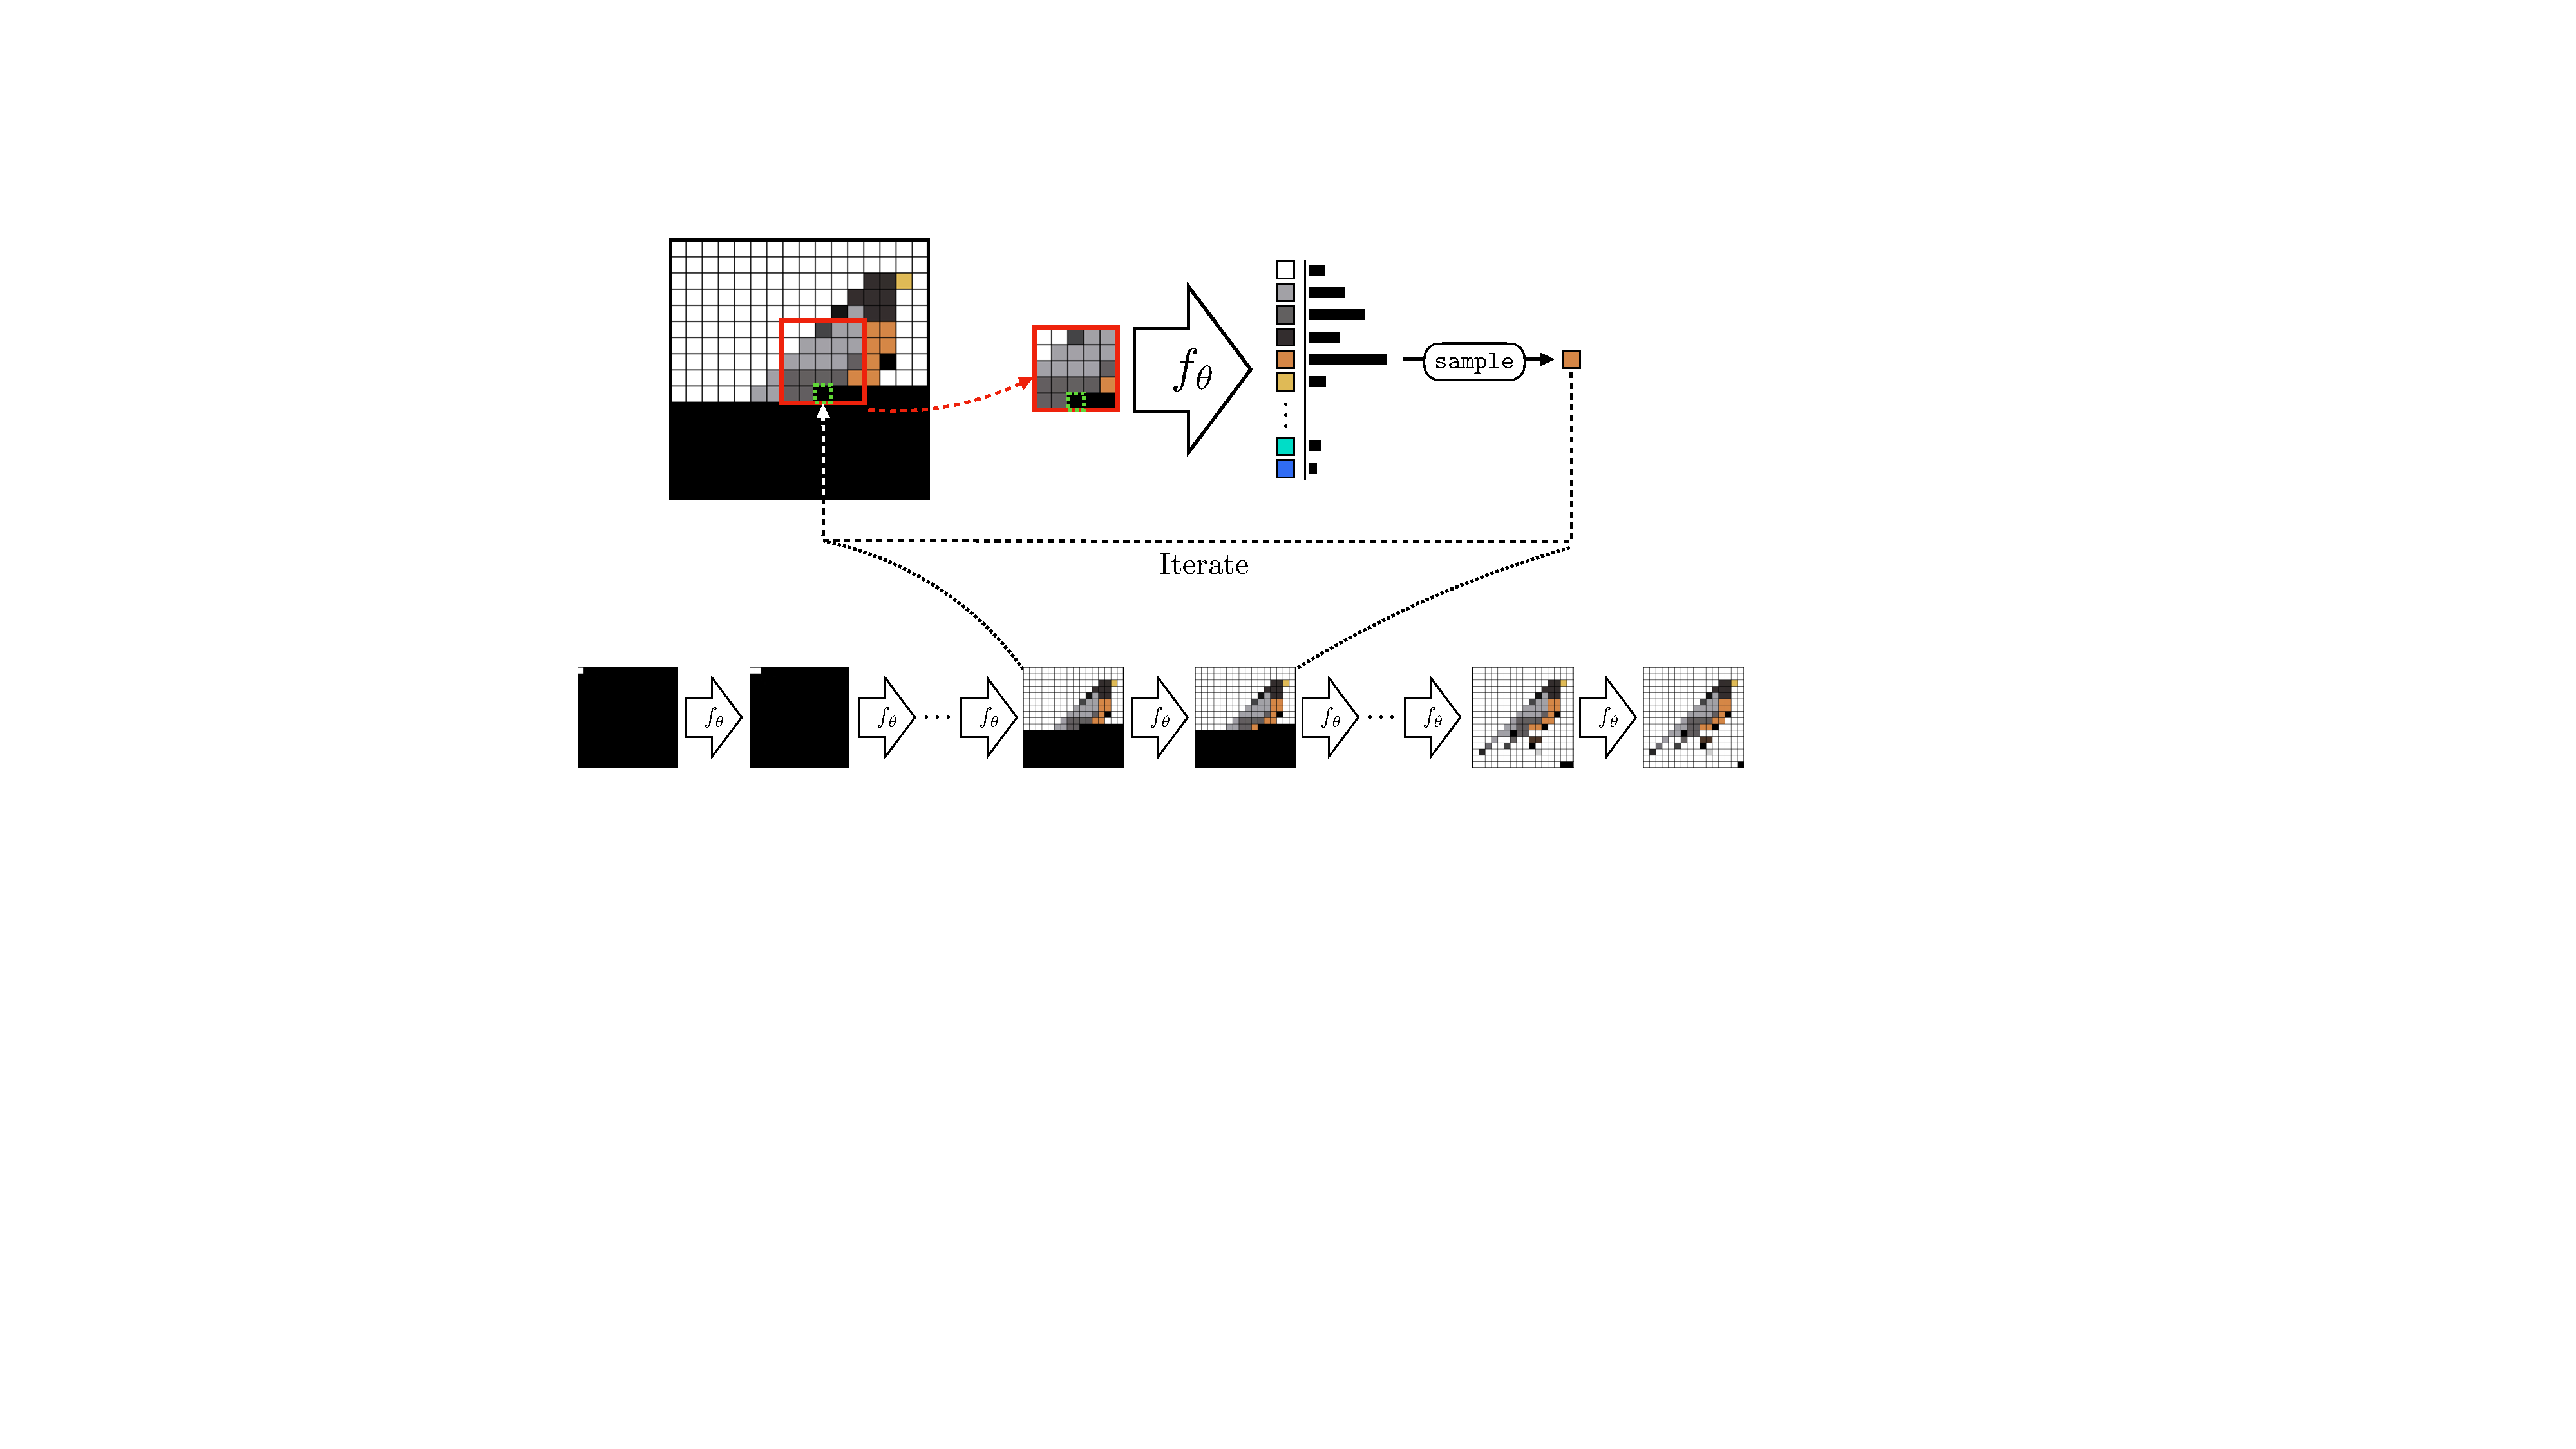
\includegraphics[width=1.0\linewidth]{./figures/generative_models/autoregressive_prediction_schematic.pdf}
    }
    \caption{An autoregressive model, $f_{\theta}$, that generates an image pixel by pixel. The black pixels are the remaining pixels to synthesize. Compare with the Efros-Leung model in \fig{\ref{fig:sampling_efros_leung}}.}
    \label{fig:generative_models:autoregressive_prediction_schematic}
\end{figure}
\marginnote{As an exercise, think about how to design a convolutional neural network that can perform the prediction problem in \fig{\ref{fig:generative_models:autoregressive_prediction_schematic}} (see the PixelCNN architecture in \cite{van2016conditional} for one solution).}[-2.6cm]

You might have noticed that this setup looks very similar to the Efros-Leung texture synthesis algorithm in \sect{\ref{sect:Efros-Leung_texture}}, and indeed that was also an autoregressive model. The Efros-Leung algorithm was a nonparametric method that worked by stealing pixels from the matching regions of an exemplar texture. Now we will see how to do autoregressive modeling with a learned, parameteric predicton function $f_{\theta}$, such as a deep net.

These models can be easily understood by first considering the problem of synthesizing one pixel, then two, and so on. The first observation to make is that it's pretty easy to synthesize a single grayscale pixel. Such a pixel can take on 256 possible values (for a standard 8-bit grayscale image). So it suffices to use a categorical distribution to represent the probability that the pixel takes on each of these possible values. The categorical distribution is fully expressive: any possible probability mass function (pmf) over the 256 values can be represented with the categorical distribution. Fitting this categorical distribution to training data just amounts to counting how often we observe each of the 256 values in the training set pixels, and normalizing by the total number of training set pixels. So, we know how to model one grayscale pixel. We can sample from this distribution to synthesize a random one-pixel image. %Autoregressive models just do this over and over for all the pixels.

How do we model the distribution over a second grayscale pixel given the first? In fact, we already know how to model this; mathematically, we are just trying to model $p(\mathbf{x_2} \given \mathbf{x_1})$ where $\mathbf{x_1}$ is the first pixel and $\mathbf{x_2}$ is the second. Treating $\mathbf{x}_2$ as a categorical variable (just like $\mathbf{x_1}$), we can simply use a softmax regression, which we saw in \sect{\ref{sec:intro_to_learning:image_classification}}. In that section we were modeling a $K$-way categorical distribution over $K$ object classes, conditioned on an input image. Now we can use exactly the same tools to model a $256$-way distribution over a the second pixel in a sequence conditioned on the first.\marginnote{In this section we index the first pixel as $\mathbf{x}_1$ rather than $\mathbf{x}_0$.}

What about the third pixel, conditioned on the first two? Well, this is again a problem of the same form: a 256-way softmax regression conditioned on some observations. Now you can see the induction: modeling each next pixel in the sequence is a softmax regression problem that models $p(\mathbf{x}_n \given \mathbf{x}_1, \ldots, \mathbf{x}_{n-1})$. We show how the cross-entropy loss can be computed in \fig{\ref{fig:generative_models:autoregressive_softmax_regression}}. Notice that it looks almost identical to \fig{\ref{fig:softmax_regression_diagram}} from \chap{\ref{chapter:intro_to_learning}}.
\begin{figure}[t]
    \centerline{
    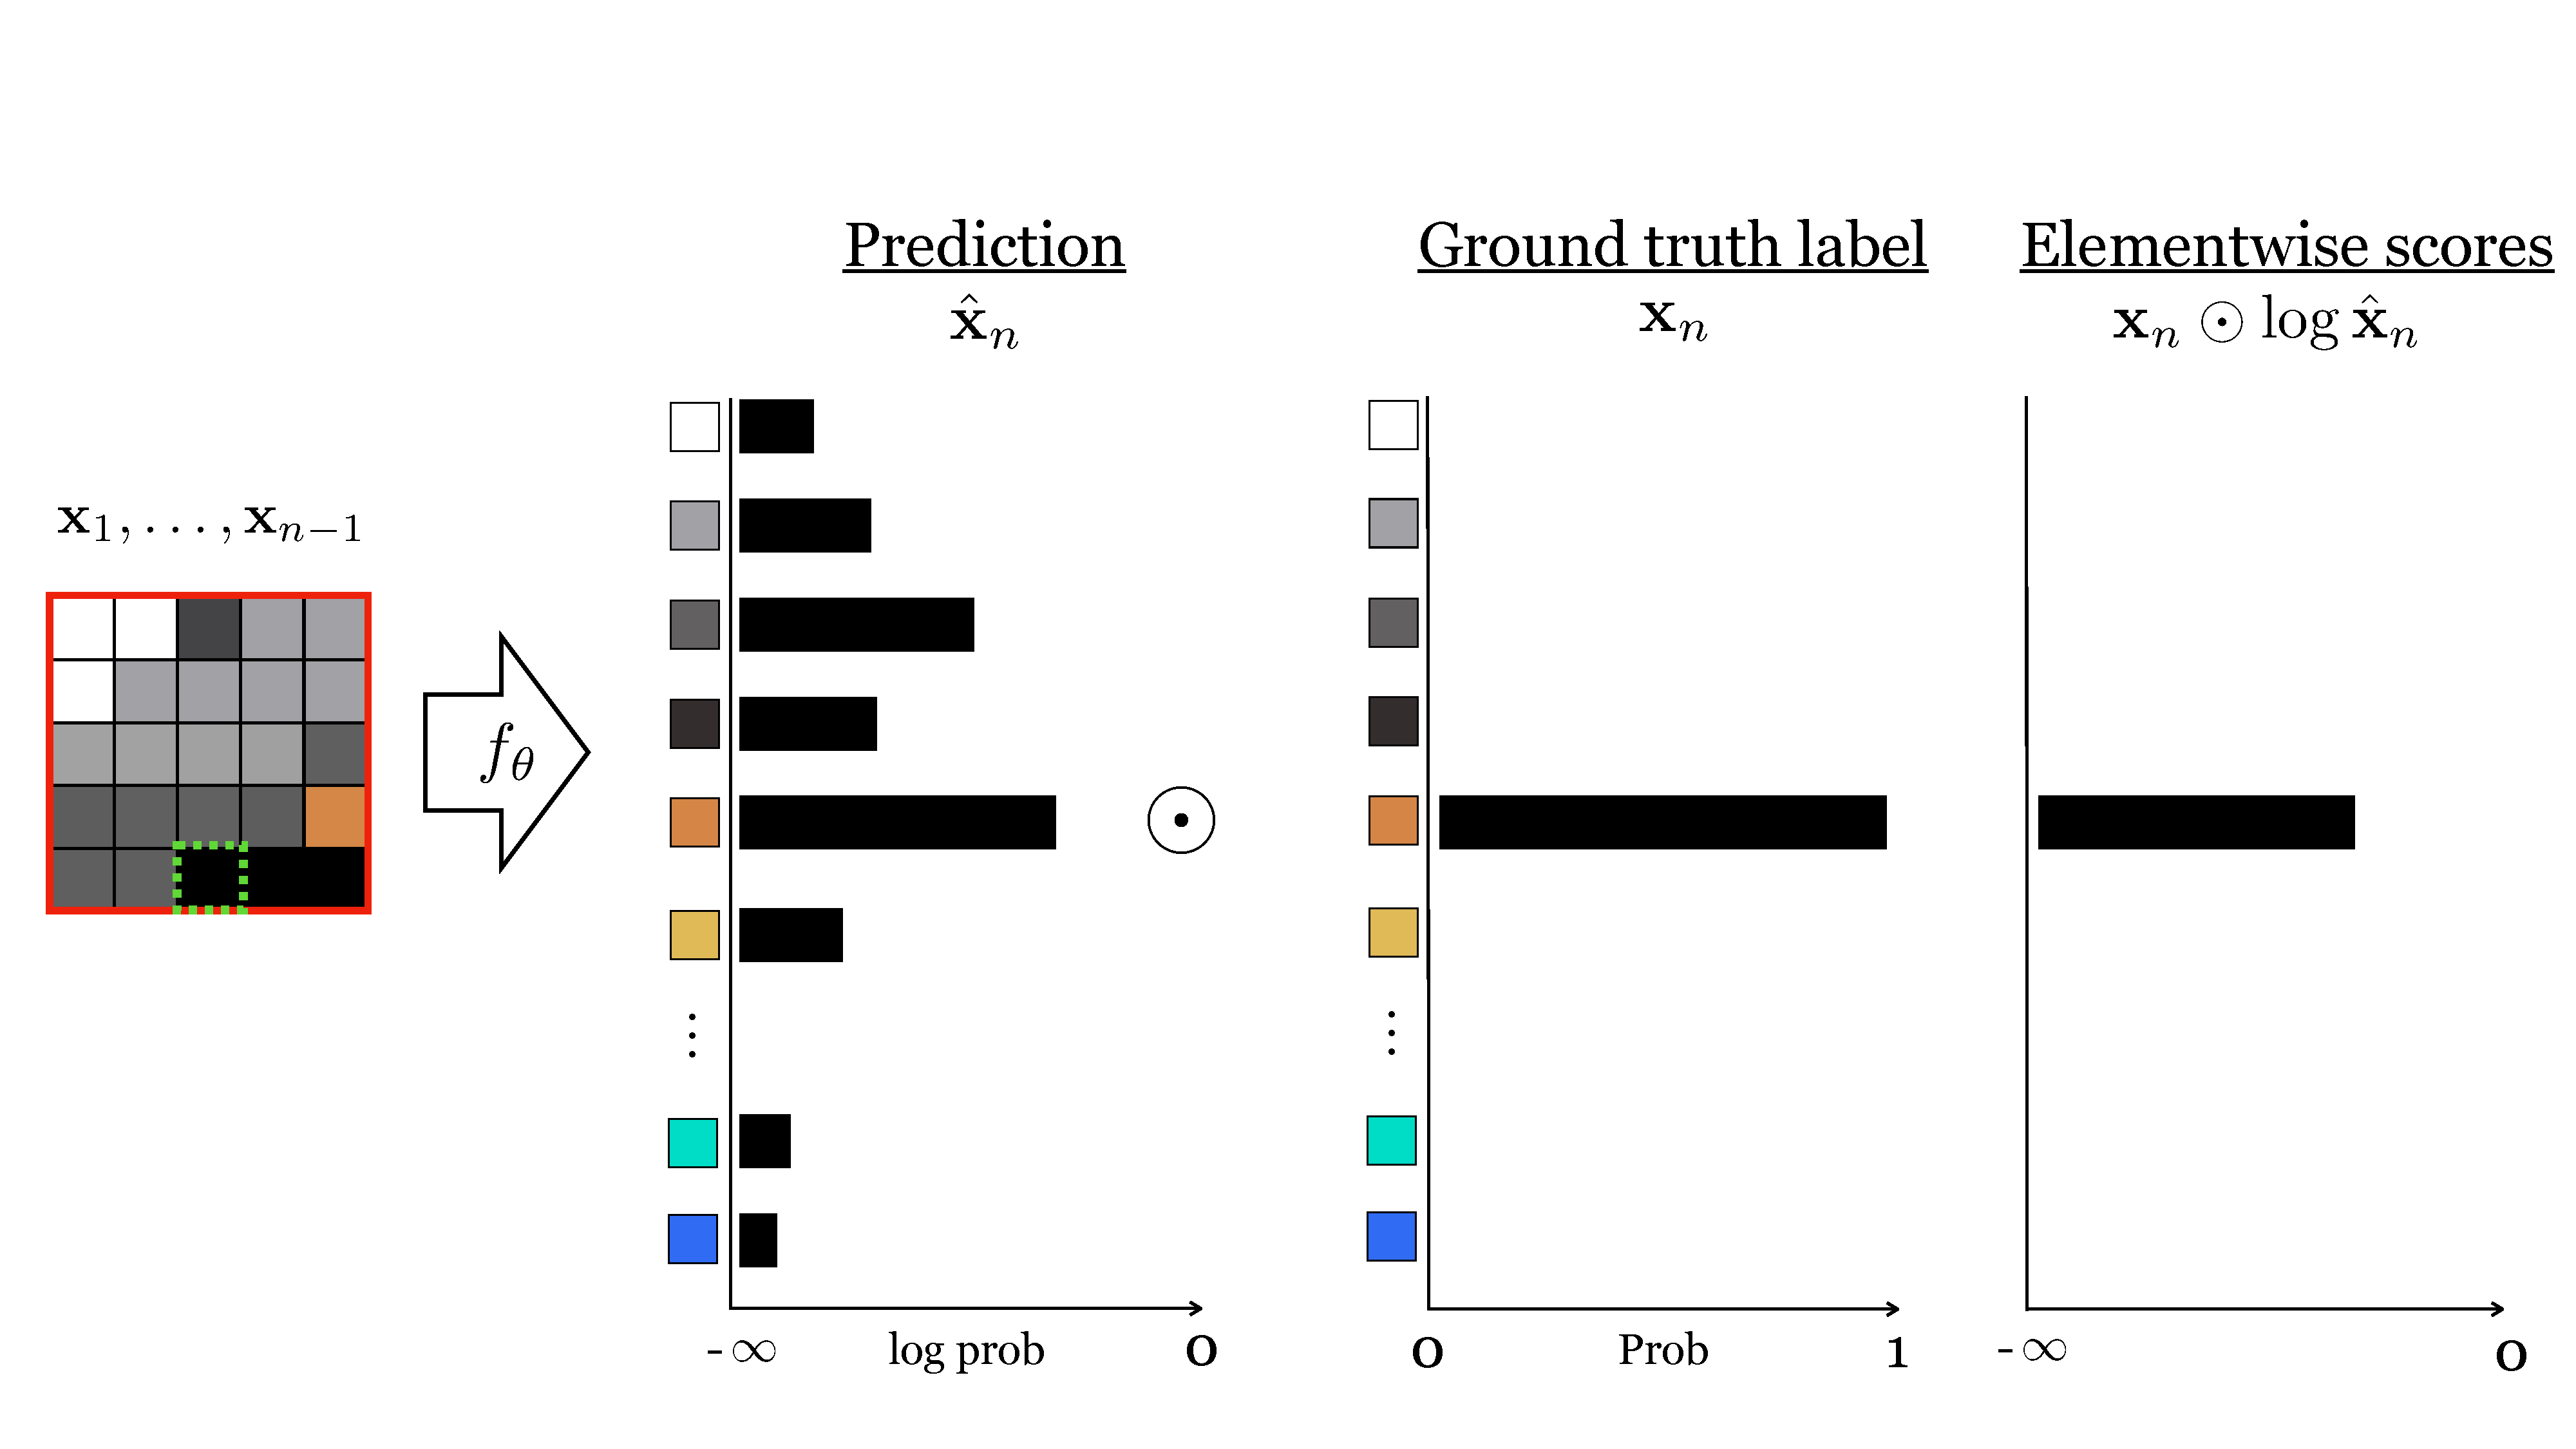
\includegraphics[width=1.0\linewidth]{./figures/generative_models/autoregressive_softmax_regression.pdf}
    }
    \caption{Autoregressive prediction as next-pixel-classification.}
    \label{fig:generative_models:autoregressive_softmax_regression}
\end{figure}
If we have color images we need to predict three values per-pixel, one for each of the red, green, and blue channels. One way to do this is to predict and sample the values for these three channels in sequence: first predict the red value as a 256-way classification problem, then sample the red value you will use, then predict the green value as a 256-way classification problem, and so on.

%The hard part is to model a structured joint distribution over $\mathbf{y} = [y_1, \ldots, y_n]$. 
You might be wondering, how do we turn an image into a sequence of pixels? Good question! There are innumerable ways, but the simplest is often good enough: just vectorize the two-dimensional (2D) grid of pixels by first listing the first row of pixels, then the second row, and so forth. In general, any fixed ordering of the pixels into a sequence is actually valid, but this simple method is perhaps the most common.

So we can model the probability of each subsequent pixel given the preceding pixels. To generate an image we can sample a value for the first pixel, then sample the second given the first, then the third given the first and second, and so forth. But is this a valid model of $p(\mathbf{X}) = p(\mathbf{x}_0, \ldots, \mathbf{x}_n)$, the probability distribution of the full set of pixels? Does this way of sequential sampling draw a valid sample from $p(\mathbf{X})$? It turns out it does, according to the {\bf chain rule of probability}. This rule allows us to factorize \textit{any} joint distribution into a product of conditionals as follows:\marginnote{As a notational convenience, we define here that $p(\mathbf{x}_i \given \mathbf{x}_1, \ldots, \mathbf{x}_{i-1}) = p(\mathbf{x}_1)$ when $i=1$.}[0.7cm]
\begin{align}
    p(\mathbf{X}) &= p(\mathbf{x_n} \given \mathbf{x_1}, \ldots, \mathbf{x}_{n-1})p(\mathbf{x}_{n-1} \given \mathbf{x}_1, \ldots, \mathbf{x}_{n-2}) \quad \ldots \quad p(\mathbf{x}_2 \given \mathbf{x}_1)p(\mathbf{x}_1)\\
    p(\mathbf{X}) &= \prod_{i=1}^n p(\mathbf{x}_i \given \mathbf{x}_1, \ldots, \mathbf{x}_{i-1})\label{eqn:generative_models:autoregressive_likelihood}
\end{align}
This factorization demonstrates that sampling from such a model can indeed be done in sequence because all the conditional distributions are independent of each other. %This sampling method is also called \textbf{ancestral sampling} (sample your ancestors first, then sample each next generation given the preceding generation).

%Now that's just a sequence of univariate predictions. So we have reduced the problem of modeling a joint distribution into a sequence of problems of modeling a single output variable, and that's a problem we know how to solve.

\subsection{Training an Autoregressive Model}
To train an autogressive a model, you just need to extract supervised pairs of desired input-output behavior, as usual. For an autoregressive model of pixels, that means extracting  sequences of pixels $\mathbf{x}_1, \ldots, \mathbf{x}_{n-1}$ and corresponding observed next pixel $\mathbf{x}_n$. These can be extracted by traversing training images in raster order. The full training and testing setup looks like this (\fig{\ref{fig:generative_models:autoregressive_train_predict}}):
\begin{figure}[h]
    \centerline{
    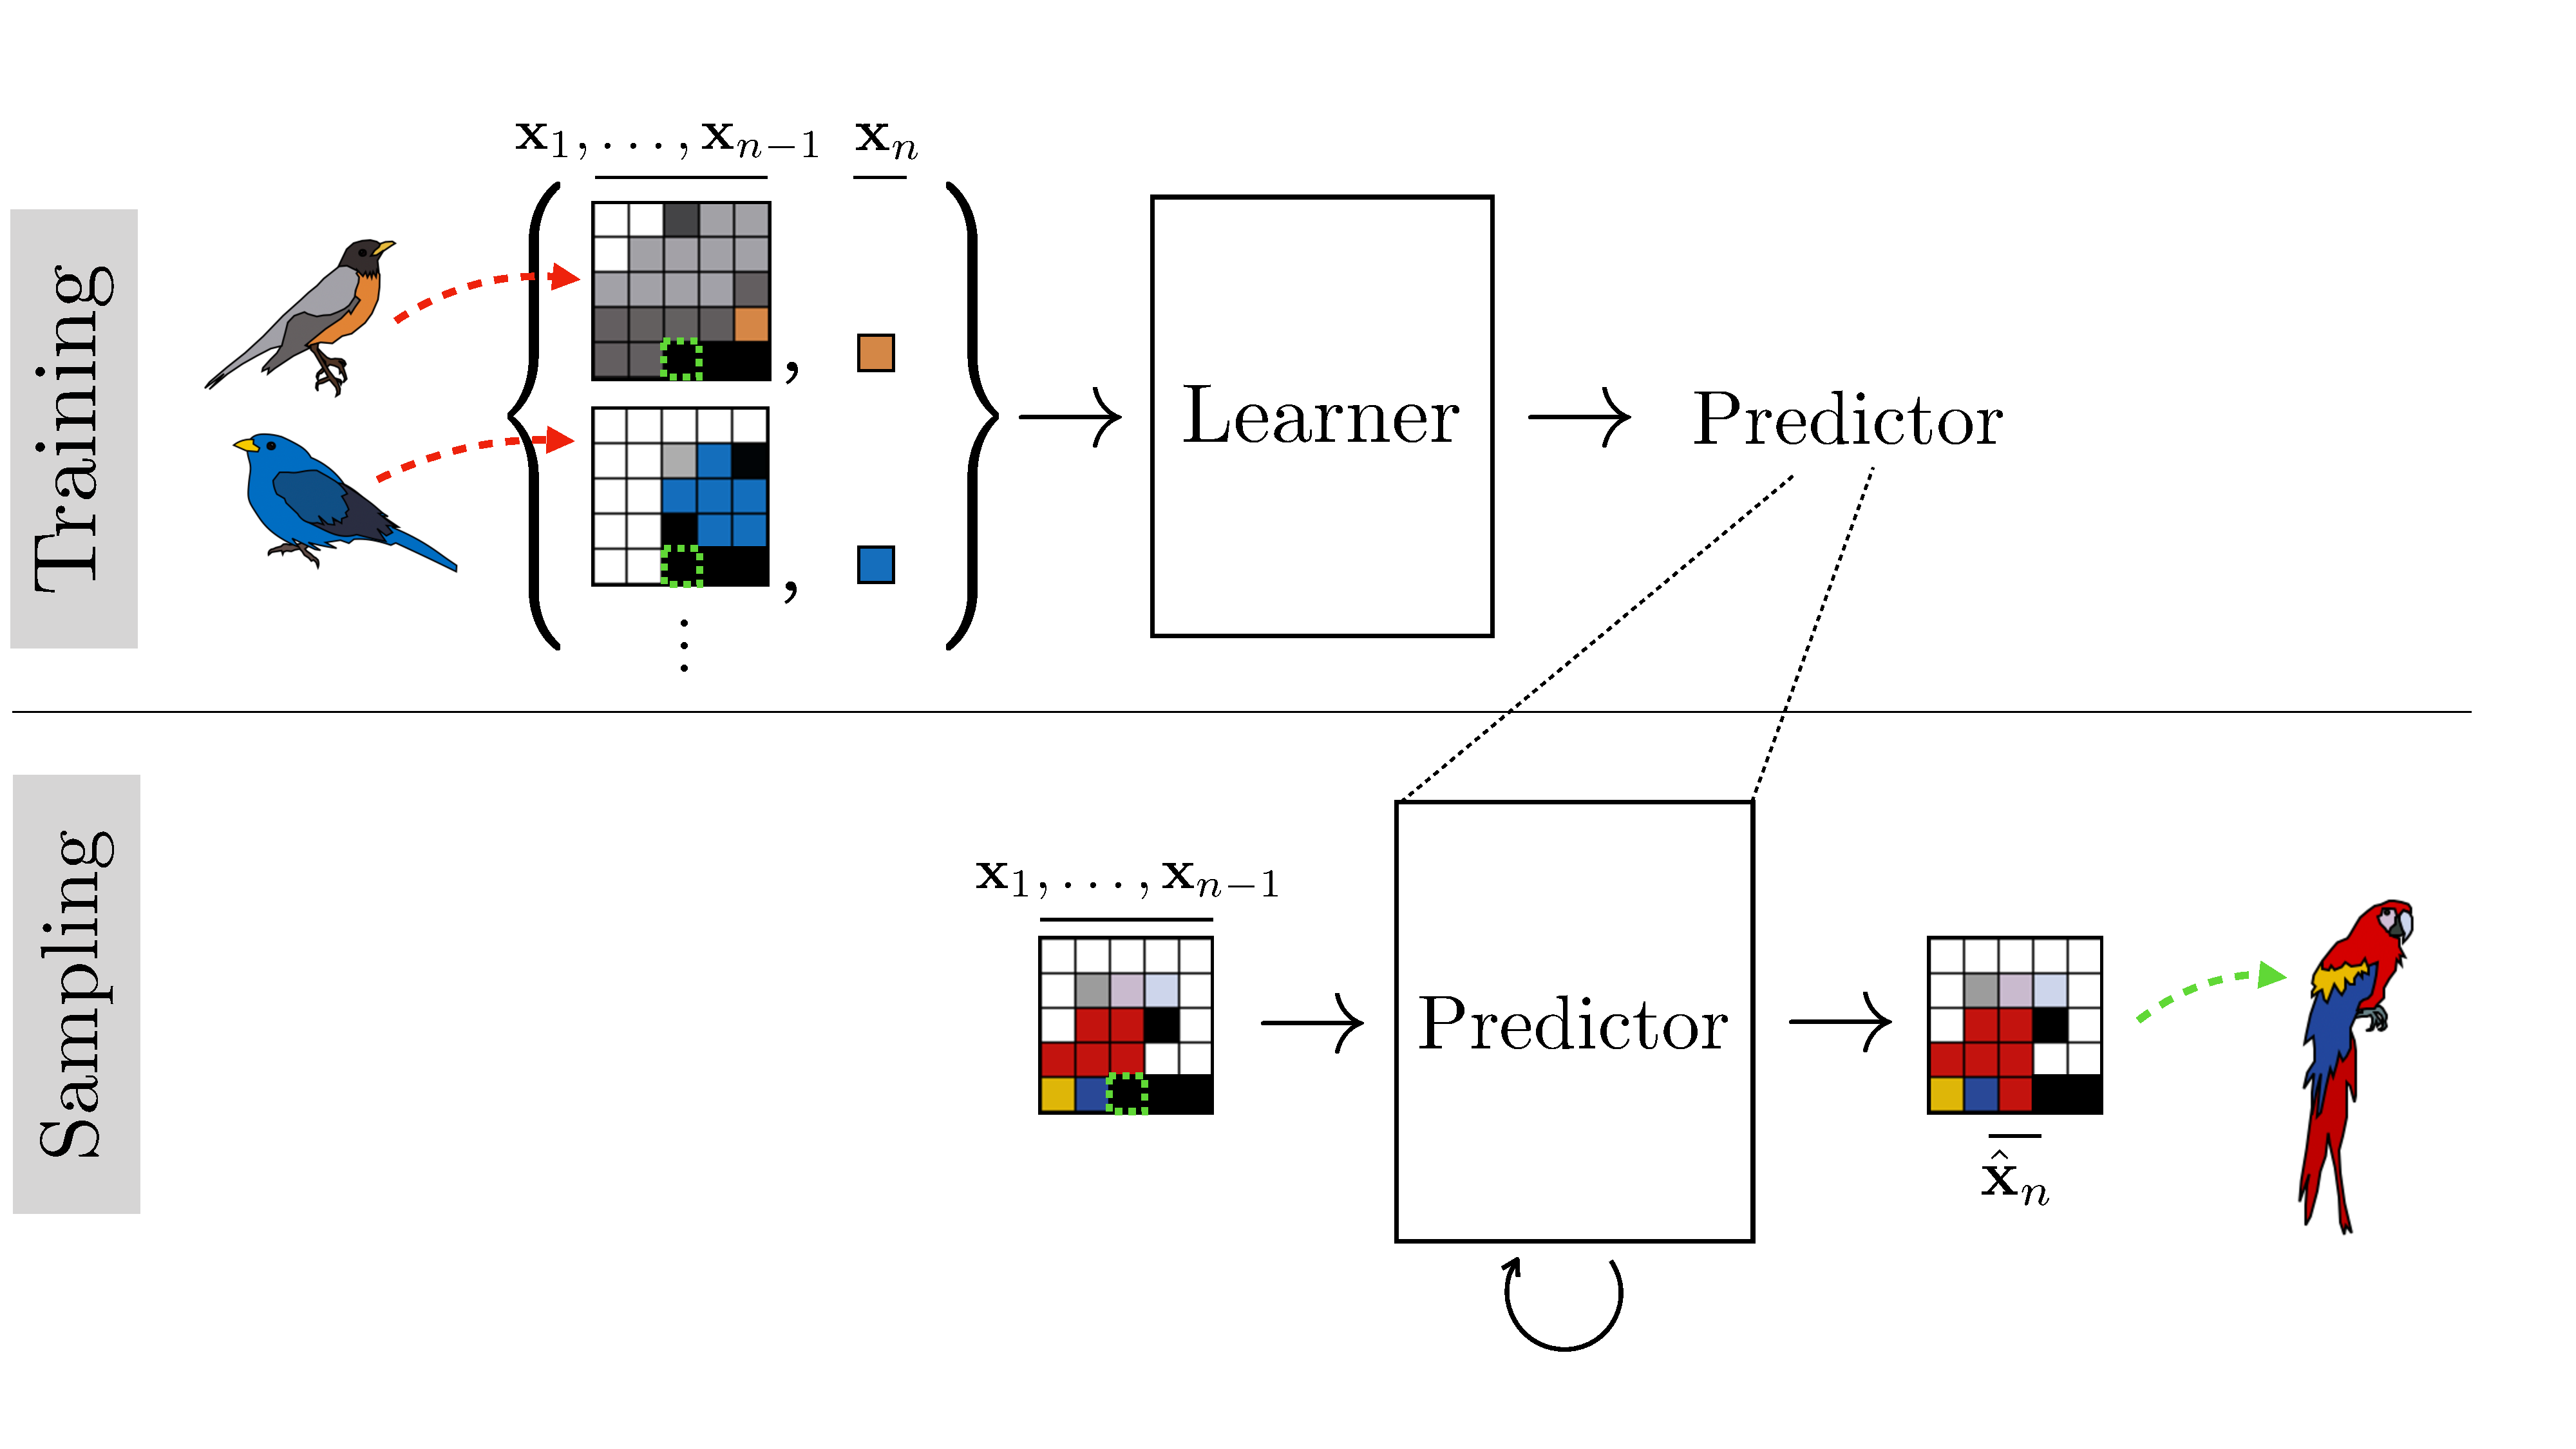
\includegraphics[width=1.0\linewidth]{./figures/generative_models/autoregressive_train_predict.pdf}
    }
    \caption{Training an autoregressive model, then sampling images from it.}
    \label{fig:generative_models:autoregressive_train_predict}
\end{figure}

It's worth noting here two different ways of setting up the training batches, one of which is much more efficient than the other. The first way is create a training batch that looks like this (we will call this a \textit{type 1 batch}):
\begin{align}
    &\texttt{input}: \mathbf{x}_k^{(i)}, \dots, \mathbf{x}_{k+n-1}^{(i)} \quad\quad \texttt{target output}: \mathbf{x}_{k+n}^{(i)}\\
    &\texttt{input}: \mathbf{x}_l^{(j)}, \dots, \mathbf{x}_{l+n-1}^{(j)} \quad\quad \texttt{target output}: \mathbf{x}_{l+n}^{(j)}\\
    &\ldots\nonumber
\end{align}
that is, we sample supervised examples ([sequence, completion] pairs) that each come from a different random starting location (indexed by $k$ and $l$) in a different random image (indexed by $i$ an $j$). 

The other way to set up the batches is like this (we will call this a \textit{type 2 batch}):
\begin{align}
    &\texttt{input}: \mathbf{x}_1^{(i)}, \dots, \mathbf{x}_{n-1}^{(i)} \quad\quad \texttt{target output}: \mathbf{x}_n^{(i)}\\
    &\texttt{input}: \mathbf{x}_2^{(i)}, \dots, \mathbf{x}_{n}^{(i)} \quad\quad \texttt{target output}: \mathbf{x}_{n+1}^{(i)}\\
    &\ldots\nonumber
\end{align}
that is, the example sequences overlap. This second way can be much more efficient. The reason is because in order to predict $\mathbf{x}_n$ from $\mathbf{x}_1, \dots, \mathbf{x}_{n-1}$, we typically have to compute representations of $\mathbf{x}_1, \dots, \mathbf{x}_{n-1}$, and these same representations can be reused for predicting the next item over, that is, $\mathbf{x}_{n+1}$ from $\mathbf{x}_2, \dots, \mathbf{x}_n$. As a concrete example, this is the case in transformers with causal attention (\sect{\ref{sec:transformers:masked_attention}}), which have the property that the representation of item $\mathbf{x}_{n}$ only depends on the items that preceded it in the sequence. What this allows us to do is \textit{share computation between all our overlapping predictions}, and this is why it makes sense to use type 2 training batches. Notice these are the same kind of batches we described in the causal attention section (see \eqn{\ref{eqn:transformers:causal_training_batches}}).

%take as input a context sequence from image $i$, $\mathbf{x}^{i}_1, \ldots, \mathbf{x}_4$, then predict $\hat{\mathbf{x}}_5$, compare the prediction to the ground truth $\mathbf{x}_5$, and backpropagate the loss; then sample an \textit{entirely new} context, . It turns out there is a much more efficient way to do it: in order to predict $\hat{\mathbf{x}}_5$, the autoregressive model had to also predict $\hat{\mathbf{x}}_1, \ldots, \hat{\mathbf{x}}_4$.

%For example, this is the case if the autoregressive model is a recurrent neural net, where the hidden state has to be updated sequentially, and, once you have computed the sequence of hidden states, making predictions for each item in the sequence requires very little compute (maybe a linear layer and a softmax). In these cases, it's much more efficient to compare each prediction $\hat{\mathbf{x}}_1, \ldots, \hat{\mathbf{x}}_5$ to the ground truth and backpropagate all five losses.   

\subsection{Sampling from Autoregressive Models}
Autogressive models give us an explicit density function, \eqn{\ref{eqn:generative_models:autoregressive_likelihood}}. To sample from this density we use \index{Ancestral sampling}{\bf ancestral sampling}, which is the process described previously, of sampling the first pixel from $p(\mathbf{x}_1)$, then, conditioned on this pixel, sampling the second from $p(\mathbf{x}_2 \given \mathbf{x}_1)$ an so forth. Since each of these densities is a categorical distribution, sampling is easy: one option is to partition a unit line segment into regions of length equal to the categorical probabilities and see where a uniform random draw along this line falls. Autogressive models do not have latent variables $\mathbf{z}$, which makes them incompatible with applications that involve extracting or manipulating latent variables.

%\paragraph{Nonparametric texture synthesis is an autoregressive model}

%\section{Latent variables}

%\section{Types of deep generative models}

% \begin{table}[]
%     \centering
%     \begin{tabular}{c|c|c}
%         Method & Generator & Critic \\
%         \hline
%         GAN & Neural net: $G_{\theta}: \mathcal{Z} \rightarrow \mathcal{X}$ & Neural net $D_{\phi}: \mathcal{X} \rightarrow \mathbb{R}$\\
%         EBM & MCMC & Neural net $E_{\theta}:\mathcal{X} \rightarrow \mathbb{R}$ \\
%         Normalizing flow & Neural net $G_{\theta}: \mathcal{Z} \rightarrow \mathcal{X}$ & Density $p_{\theta}: \mathcal{X} \rightarrow [0,1], p_{\theta}(\mathbf{x}) = p_{\mathbf{z}}(G_{\theta}^{-1}(\mathbf{x}))|\det(\frac{\partial G_{\theta}^{-1}(\mathbf{x})}{\partial \mathbf{x}})|$ \\
%         VAE & Neural net: $G_{\theta}: \mathcal{Z} \rightarrow \mathcal{X}$ & Reconstruction error: $\mathcal{X} \rightarrow \mathbb{R}, \norm{G_{\theta}(F_{\phi}(\mathbf{x}))-\mathbf{x}}$\\
%         Autoregressive & Ancestral sampling & Density $p_{\theta}: \mathcal{X} \rightarrow [0,1], p_{\theta}(\mathbf{x}) = \prod_i p_{\theta}(x_i | x_1, \ldots, x_{i-1})$ & \\
%     \end{tabular}
%     \caption{}
%     \label{tab:my_label}
% \end{table}

%The field of deep generative modeling is rapidly evolving. We will next cover five families of model that are currently popular, but if you are reading this in a few years, it's likely a whole host of new models will exist. The important thing to notice is how all these models stem from the same ingredients, just used in slightly different proportions and combinations. As you read these sections look for the commonalities. For example, which of the models are optimizing a likelihood function? Which are based on a factorization of a joint probability distribution. Which use sampling to approximate intractable integrals? And so forth. The next generation of models will likely be minor variations on these themes, just as this generation of models can be viewed as minor variations on older models.% from the fields of statistics~\cite{XX}, physics~\cite{XX}, and economics~\cite{XX}.

\section{Diffusion Models}\label{sec:generative_models:diffusion_models}
\index{Diffusion model}
The strategy of autoregressive models is to break a hard problem into lots of simple pieces. \textbf{Diffusion models} are another class of model that uses this same strategy~\cite{sohl2015deep}. They can be easy to understand if we start by looking at what autoregressive models do in the \textit{reverse} direction: starting with a complete image, they remove one pixel, then the next, and the next (\fig{\ref{fig:generative_models:reverse_autoregressive_sequence}}):
\begin{figure}
    \centerline{
        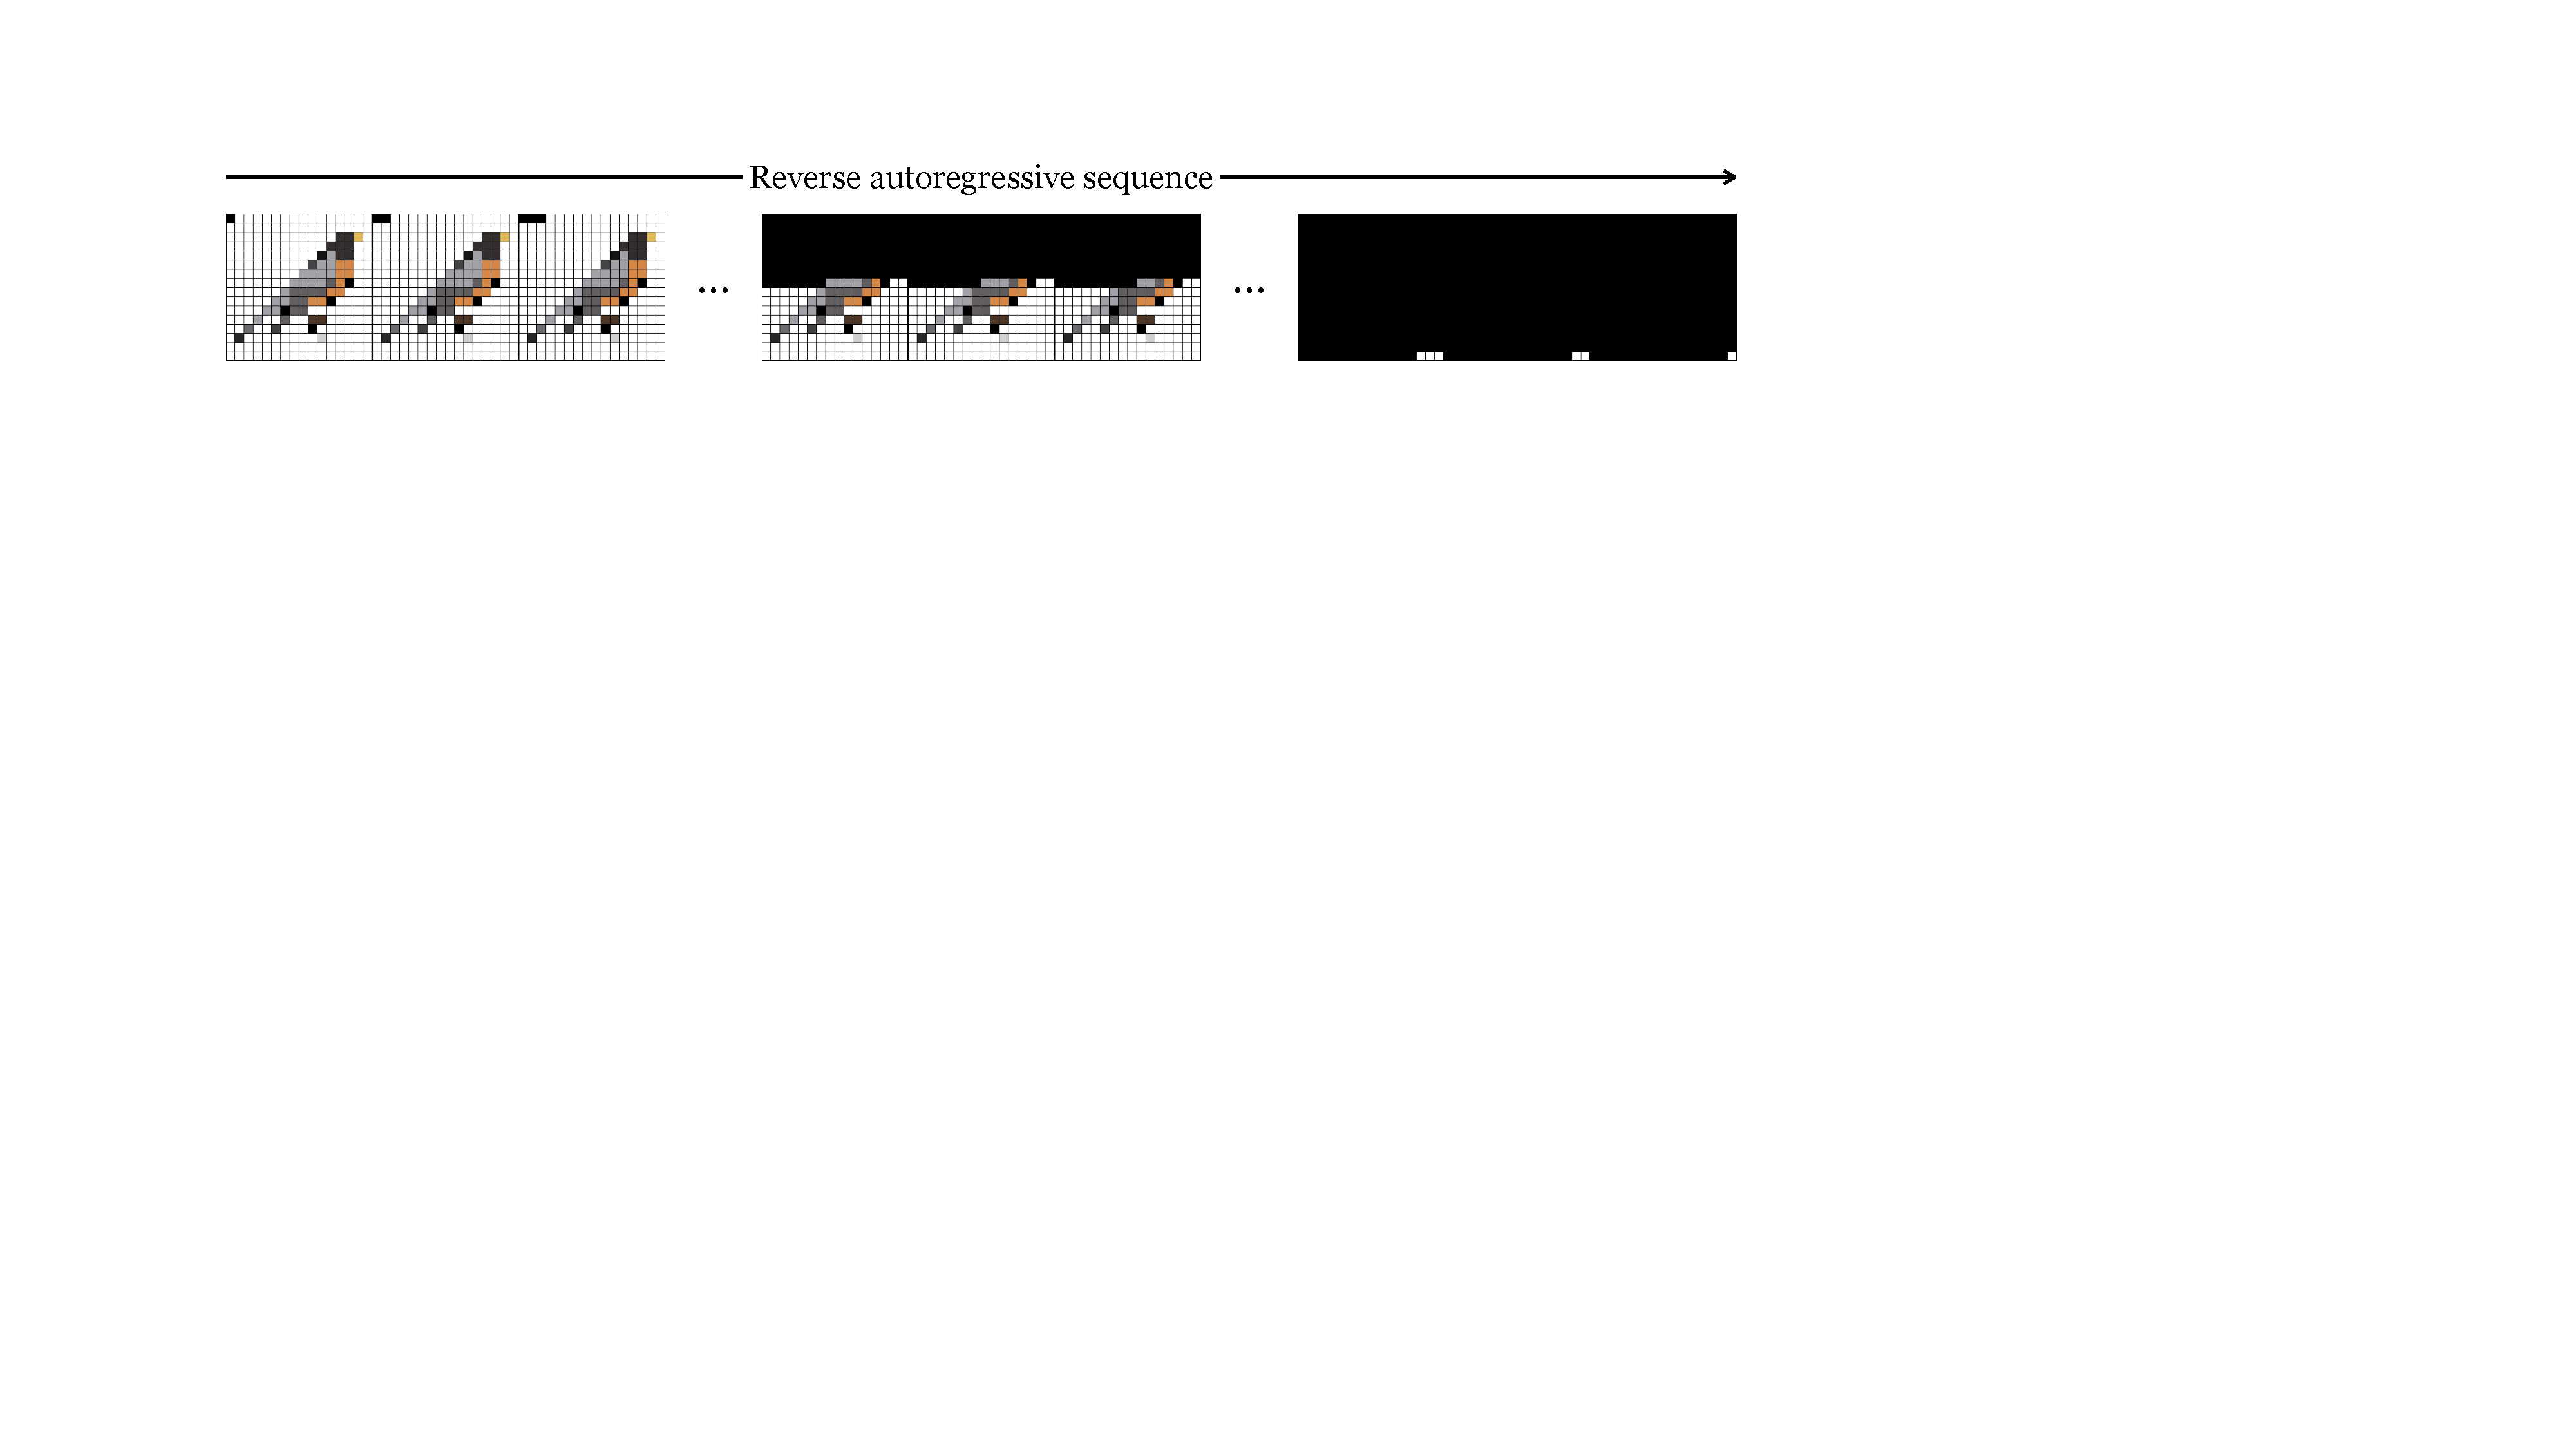
\includegraphics[width=1.0\linewidth]{./figures/generative_models/reverse_autoregressive_sequence.pdf}
    }
    \caption{An autoregressive sequence in reverse is a corruption process that removes one pixel at a time.}
    \label{fig:generative_models:reverse_autoregressive_sequence}
\end{figure}

This is a \textit{signal corruption} process. The idea of diffusion models is that this is not the only corruption process we could have used, and maybe not the best. Diffusion models instead use the following corruption process: starting with an uncorrupted image, $\mathbf{x}_0$, they add noise $\mathbf{\epsilon}_0$ to this image, resulting in a noisy version of the image, $\mathbf{x}_1$. Then they repeat this process, adding noise $\mathbf{\epsilon}_1$ to produce an even noisier signal $\mathbf{x}_2$, and so on. Most commonly, the noise is isotropic Gaussian noise. \Fig{\ref{fig:generative_models:forward_diffusion_process}} shows what that looks like:
\begin{figure}
    \centerline{
        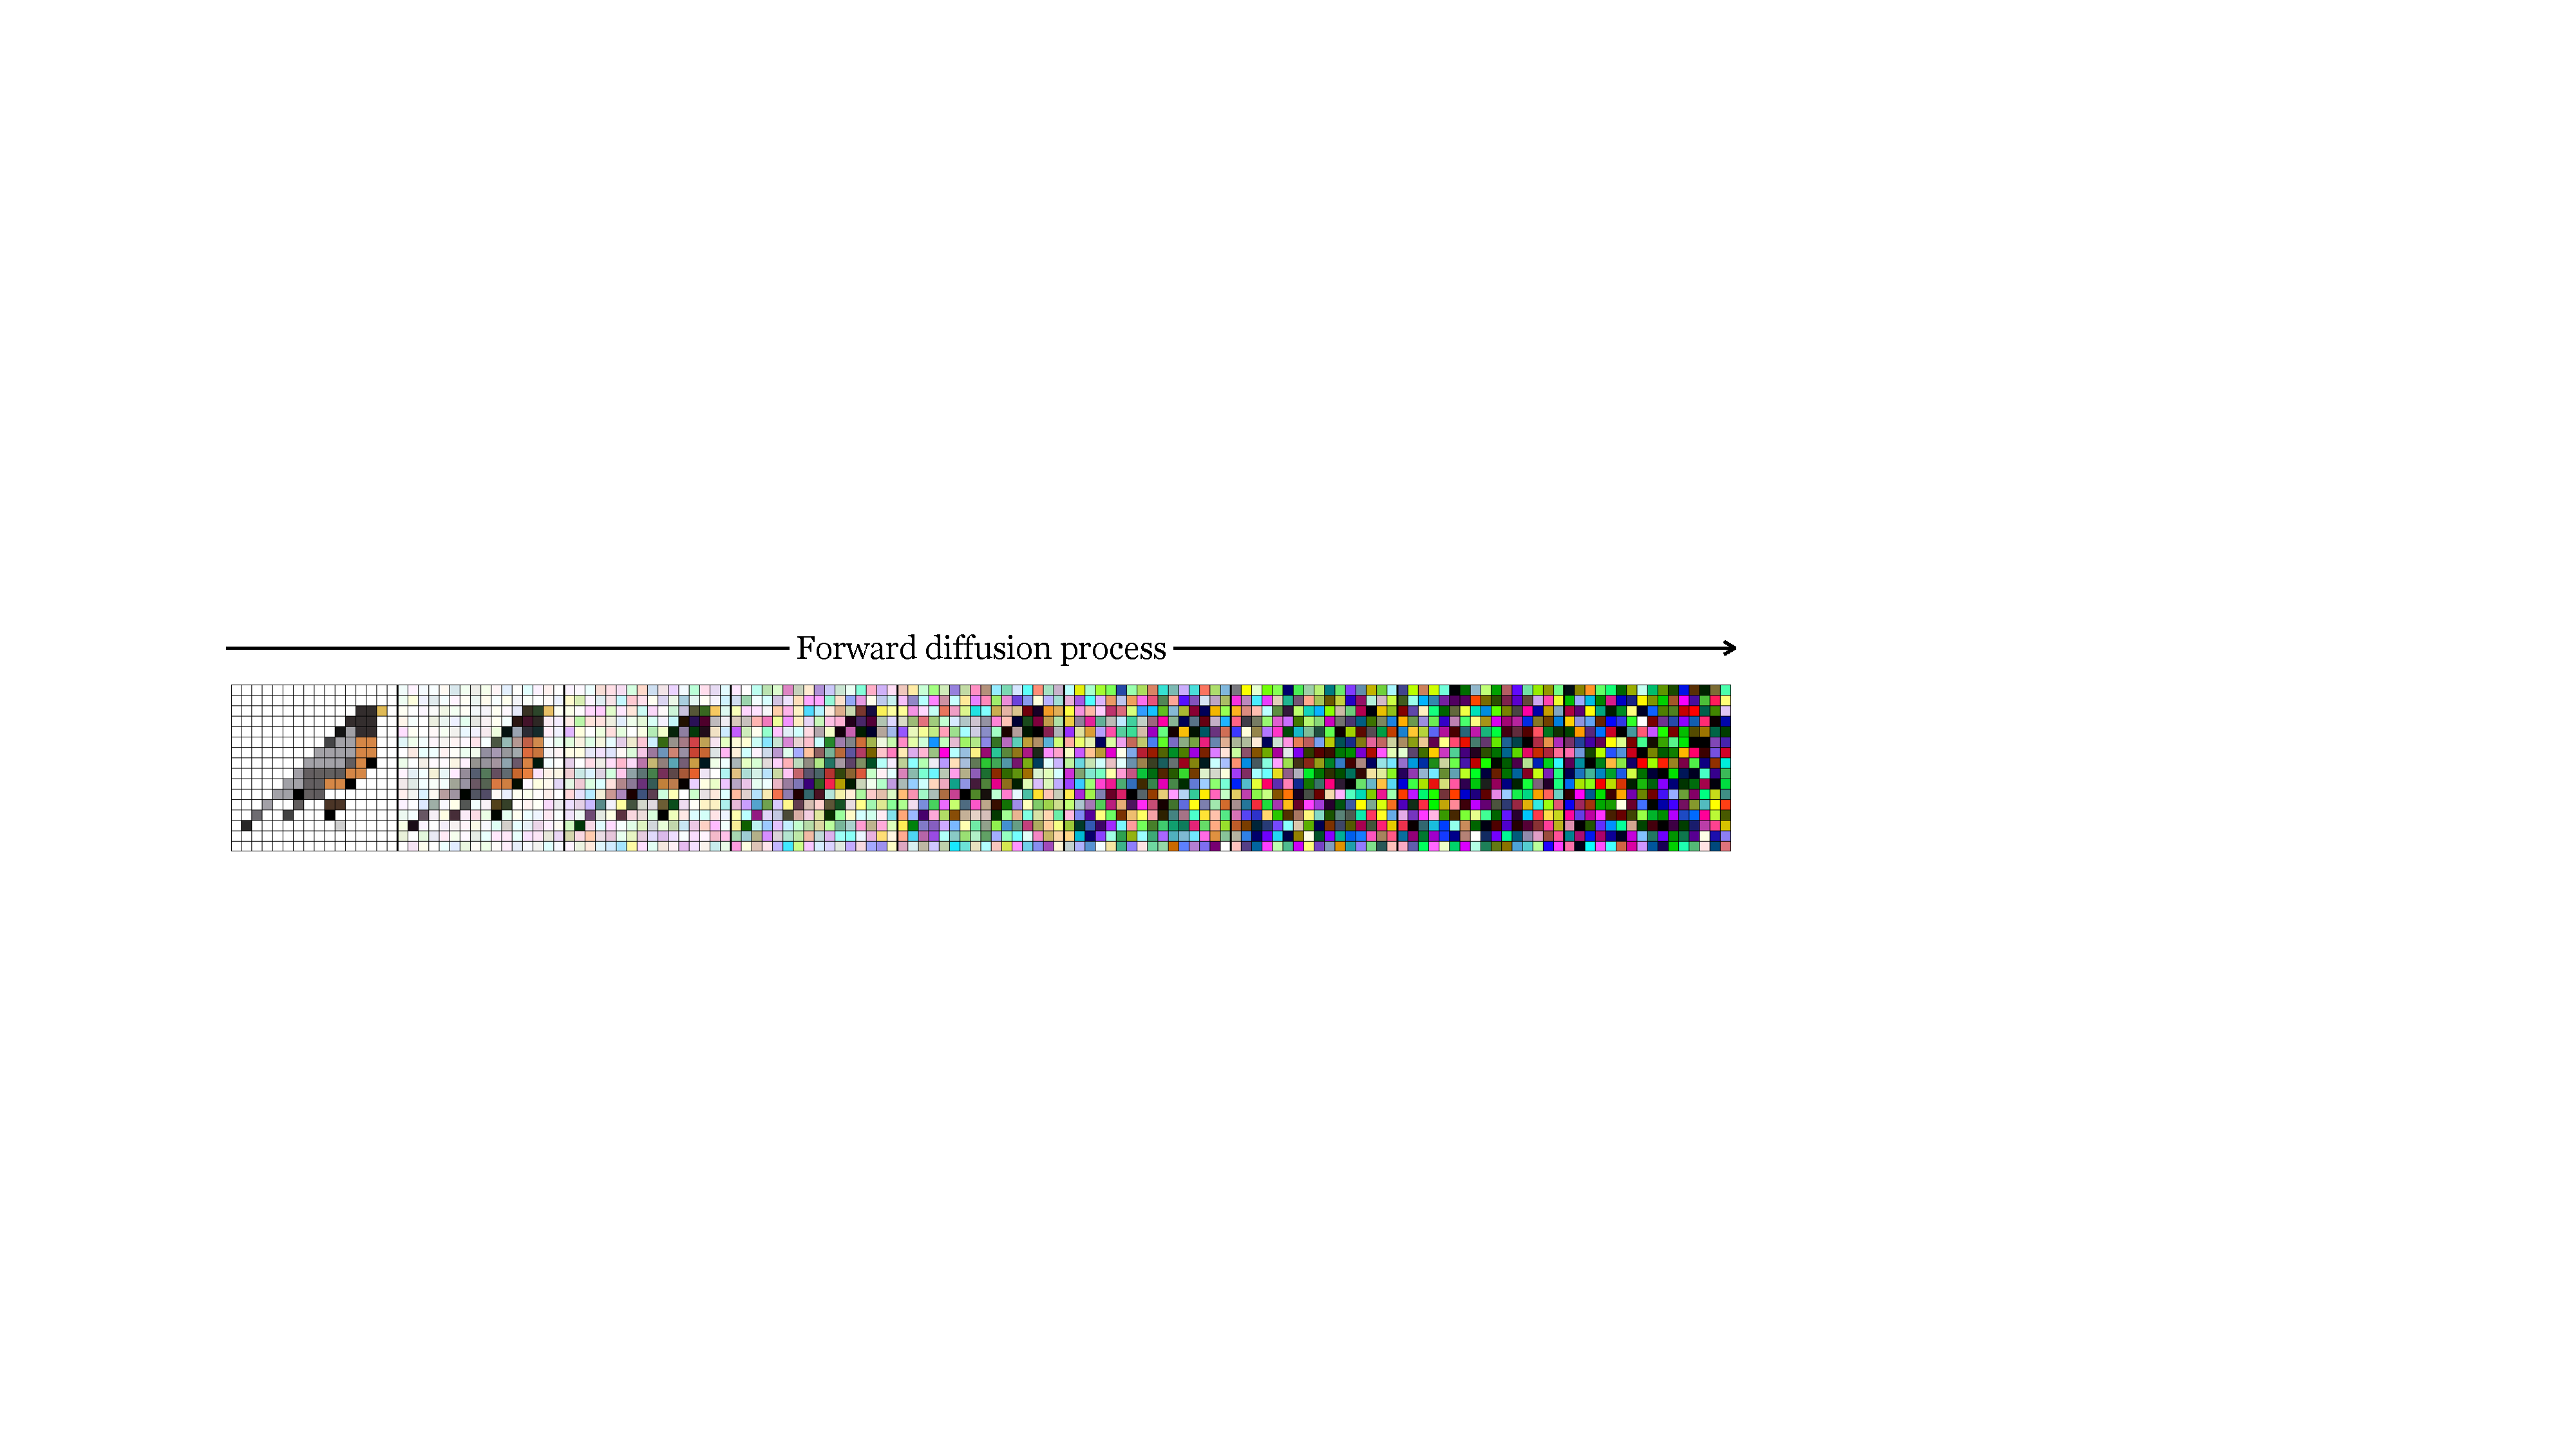
\includegraphics[width=1.0\linewidth]{./figures/generative_models/forward_diffusion_process.pdf}
    }
    \caption{Forward diffusion process.}
    \label{fig:generative_models:forward_diffusion_process}
\end{figure}

After $T$ steps of this process, the image $\mathbf{x}_T$ looks like pure noise, if $T$ is large enough. In fact, if we use the following noise process, then $\mathbf{x}_T \sim \mathcal{N}(\mathbf{0},\mathbf{I})$ as $T \rightarrow \infty$ (which follows from equation 4 in \cite{ho2020denoising}).
\begin{align}
    \mathbf{x}_t &= \sqrt{(1-\beta_t)}\mathbf{x}_{t-1} + \sqrt{\beta_t}\mathbf{\epsilon}_t\\
    \epsilon_t &\sim \mathcal{N}(\mathbf{0},\mathbf{I})
\end{align}
The $\beta_t$ values should be $\leq 1$ and can be fixed for all $t$ (like in the previous equations) or can be set according to some schedule that changes the amount of noise added over time.


%What if instead we remove several pixels at a time, and in a random order? Then the corruption sequence looks like this:

%We can train a net to reverse this process, and that net will then end up synthesizing an image, incrementally, starting from an empty image. Such a net will not quite follow \eqn{\ref{eqn:generative_models:autoregressive_likelihood}} because several variables are sampled at a time. However, if we assume that these variables are independent then the equation remains valid:
%\begin{align}
%    p(\mathbf{X}) &= \prod_{i=1}^n p(\mathbf{x}_i | \mathbf{x}_1, \ldots, \mathbf{x}_{i-1})
%    &\approx \prod_{i=1}^n p(\mathbf{x}_i | \mathbf{x}_1, \ldots, \mathbf{x}_{i-1})
%\end{align}

%Therefore, this kind of autoregressive model corresponds to assuming independence between the pixels we are decoding on each step. This is called \textbf{parallel decoding} and shows up in models such as \cite{maskgit} and \cite{muse}.

%Diffusion models run parallel decoding over \textit{all} pixels at once. However, instead of predicting pixels wholesale, they predict small perturbations.

%The corruption process of a (Gaussian) diffusion model is to add Gaussian noise at each step. Repeating this process enough time results in an image that is pure noise -- with proper scaling and centering the limit of the noising process is $\mathcal{N}(0,1)$.

Now, just like autoregressive models, diffusion models train a neural net, $f_{\theta}$, to \textit{reverse} this process. It can be trained via supervised learning on examples sequences of different images getting noisier and noisier. For example, as shown below in \fig{\ref{fig:generative_models:reverse_diffusion_process}}, the sequence of images of the bird getting noisier and noisier can be flipped in time and thereby provide a sequence of \textit{training examples} of the mapping $\mathbf{x}_t \rightarrow \mathbf{x}_{t-1}$, and these examples can be fit by a predictor $f_{\theta}$.
\begin{figure}
    \centerline{
        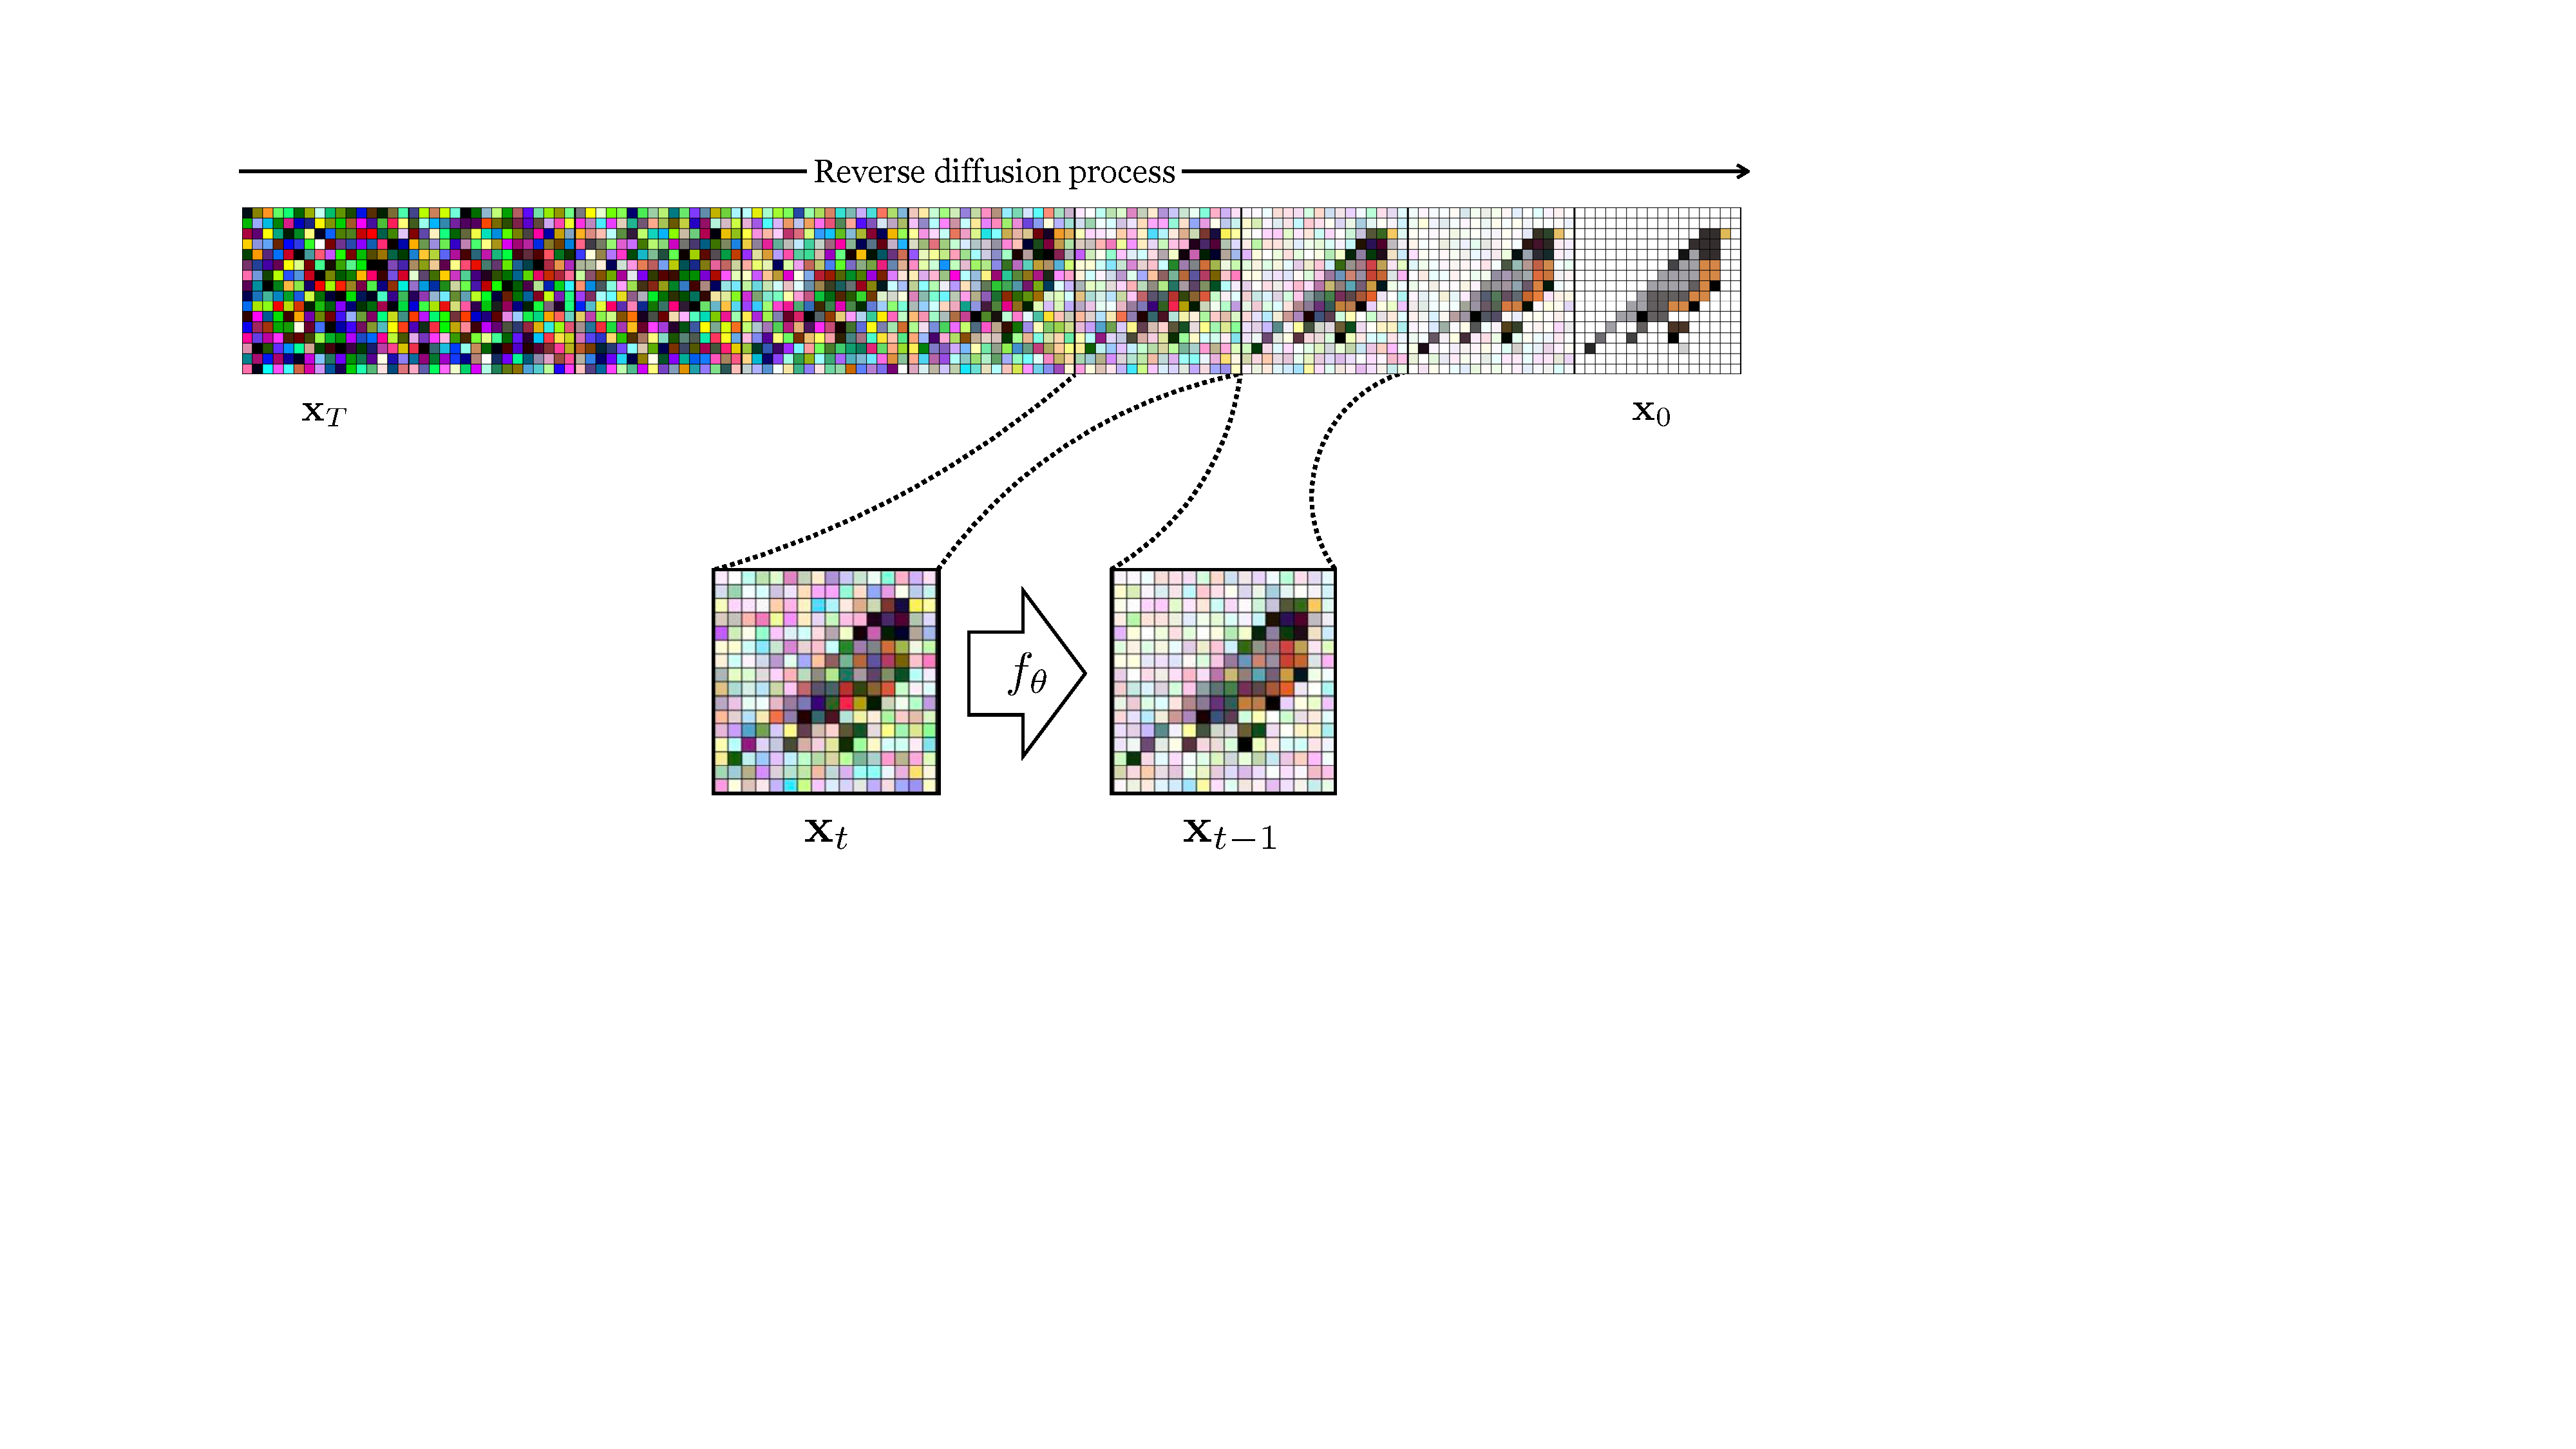
\includegraphics[width=1.0\linewidth]{./figures/generative_models/reverse_diffusion_process.pdf}
    }
    \caption{Reverse diffusion process. The forward process creates supervision to train the reverse process.}
    \label{fig:generative_models:reverse_diffusion_process}
\end{figure}

\marginnote{Notice the similarity between this reverse diffusion process and the Heeger-Bergen algorithm from \chap{\ref{chap:textures}} (\fig{\ref{fig:heeger_bergen_iterations}}). Both algorithms start with a noise input and iteratively refine it until it looks like a real image.}[-4.4cm]

We call $f_{\theta}$ a \textbf{denoiser}; it learns to remove a little bit of noise from an image. If we apply this denoiser over and over, starting with pure noise, the process should coalesce on a noise-less image that looks like one of our training examples. The steps to train a diffusion model are therefore as follows:
\begin{enumerate}
    \item Generate training data by corrupting a bunch of images (forward process; noising).
    \item Train a neural net to invert each step of corruption (reverse process; denoising).
\end{enumerate}
As an additional trick, it can help to let the denoising function observe time step $t$ as input, so that we have,
\begin{align}
    \hat{\mathbf{x}}_{t-1} = f_{\theta}(\mathbf{x}_t, t)
\end{align}
This can help the denoiser to make better predictions, because knowing $t$ helps us know if we are looking at a normal scene that has been corrupted by our noise (if $t$ is large this is likely) or a scene where the actual physical structure is full of chaotic, rough textures that happen to look like noise (if $t$ is small this is more likely, because for small $t$ we haven't added much noise to the scene yet).
\Algref{\ref{alg:generative_models:diffusion_model}} presents these steps in more formal detail.
\begin{algorithm}[h]
\SetAlgoVlined
\DontPrintSemicolon
%\marginnote{{\bf Algorithm \ref{alg:generative_models:diffusion_model}}: Training a diffusion model consists of first producing training pairs of the form \{noisy image, less noisy image\}. Then do supervised learning on these pairs.}
\caption{{\bf Algorithm \ref{alg:generative_models:diffusion_model}}: Training a diffusion model consists of first producing training pairs of the form \{noisy image, less noisy image\}. Then do supervised learning on these pairs.}
\fakealgorithmcaption{}
\label{alg:generative_models:diffusion_model}
{\bf Input:} training data $\{\mathbf{x}^{(i)}\}^N_{i=1}$\;
{\bf Output:} trained model $f_{\theta}$\;
{\bf Generate training sequences via diffusion:}\;
    \For{\upshape $i=1, \dots, N$} {
        \For{\upshape $t=1, \dots, T$} {
            $\epsilon_t \sim \mathcal{N}(\mathbf{0},\mathbf{I})$\;
            $\mathbf{x}^{(i)}_t \leftarrow \sqrt{(1-\beta_t)}\mathbf{x}^{(i)}_{t-1}  + \sqrt{\beta_t}\mathbf{\epsilon}_t$
        }
    }\;
{\bf Train denoiser $f_{\theta}$ to reverse these sequences:}\;
    $\theta^* = \argmin_{\theta} \sum^N_{i=1} \sum^T_{t=1} \mathcal{L}(f_{\theta}(\mathbf{x}_t^{(i)}, t), \mathbf{x}^{(i)}_{t-1})$\;
{\bf Return:} $f_{\theta^*}$\;
\end{algorithm}

In \algref{\ref{alg:generative_models:diffusion_model}} we train the denoiser using a loss $\mathcal{L}$, which could be the $L_2$ distance. In many diffusion models, $f_{\theta}$ is instead trained to output the parameters (mean and variance) as a Gaussian density model fit to the data. This formulation yields useful probabilistic interpretations (in fact, such a diffusion model can be framed as a variational autoencoder, which we will see in \chap{\ref{chapter:generative_modeling_and_representation_learning}}). However, diffusion models can still work well without these nice interpretations, instead using a wide variety of prediction models for $f_{\theta}$~\cite{bansal2022cold}.

%We can choose different probability models for the densoiser. An autorgressive model uses a categorical distribution parameterized via a softmax over neural net logits. A (Gaussian) diffusion model instead uses a Gaussian distribution parameterized by a mean and variance per pixel output by a neural net.\marginnote{Of course this is just the vanilla version of each model, and you could imagine other choices, such as a diffusion model that uses a mixture of Gaussians over each pixel.}

%An important difference between diffusion models and autoregressive models is that autoregressive models can be exact; for an autoregressive model of 8-bit color images, the true solution, $p_{\texttt{data}}$ is in the hypothesis space if the logits are 256-dimensional. On the other hand, diffusion models are typically only approximate, in the sense that $p_{\texttt{data}}$ is not in the hypothesis space.

One useful trick for training diffusion models is to reparameterize the learning problem as predicting the noise rather than the signal~\cite{ho2020denoising}:
\begin{align}
    f_{\theta}(\mathbf{x}_t, t) &= \epsilon_t &\quad\quad \triangleleft \quad\text{first predict noise}\\
    \hat{\mathbf{x}}_{t-1} &= \mathbf{x}_t + \epsilon_t &\quad\quad \triangleleft \quad\text{then remove this noise}
\end{align}

One way to look at diffusion models is that we want to learn a mapping from pure noise (e.g., $\mathbf{z} \sim \mathcal{N}(\mathbf{0},\mathbf{I})$) to data. It is very hard to figure out how to create structured data out of noise, but it is easy to do the reverse, turning data into noise. So diffusion models turn images into noise in order to \textit{create the training sequences} for a process that turns noise into data.

\section{Generative Adversarial Networks}\label{sec:generative_models:GANs}
\index{Generative adversarial network}

Autoregressive models and diffusion models sample simple distributions step by step to build up a complex distribution. Could we instead create a system that directly, in one step, outputs samples from the complex distribution. It turns out we can, and one model that does this is the {\bf generative adversarial network} ({\bf GAN}), which was introduced by \cite{goodfellow2014generative}.

Recall that the goal of generative modeling is to make synthetic data that looks like real data. We stated previously that there are many different ways to measure ``looks like'' and each leads to a different kind of generative model. GANs take a very direct and intuitive approach: synthetic data looks like real data if a classifier cannot distinguish between synthetic images and real images.

GANs consist of two neural networks, the \textbf{generator}, $g_{\theta}: \mathcal{Z} \rightarrow \mathcal{X}$, which synthesizes data from noise, and a \index{Discriminator}\textbf{discriminator}, $d_{\phi}: \mathcal{X} \rightarrow \Delta^1$, which tries to classify between synthesized data and real data.\marginnote{Notice that $d_{\phi}$ has a form similar to an energy function, but, unlike energy functions, $d_{\phi}$ is not, in general, interpretable as an unnormalized probability density. Nonetheless, we can roughly think of a GAN as a type of energy-based generative model where we train another network $g_{\theta}$ to directly sample from the energy function rather than relying on MCMC to sample from the energy function.}[-3.0cm]

The $g_{\theta}$ and $d_{\phi}$ play an adversarial game in which $g_{\theta}$ tries to become better and better at generating synthetic images while $d_{\phi}$ tries to become better and better at detecting any errors $g_{\theta}$ is making. The learning problem can be written as a minimax game:
\begin{align}
    \argmin_\theta\max_\phi \mathbb{E}_{\mathbf{x} \sim p_{\texttt{data}}}[\log d_{\phi}(\mathbf{x})] + \mathbb{E}_{\mathbf{z} \sim p_{\mathbf{z}}}[\log (1-d_{\phi}(g_{\theta}(\mathbf{z})))]\label{eqn:generative_models:GAN_learning_problem}
\end{align}

Schematically, the generator synthesizes images that are then fed as input to the discriminator. The discriminator tries to assign a high score to generated images (classifying them as synthetic) and a low score to real images from some training set (classifying them as real), as shown in \fig{\ref{fig:generative_models:generative_models:gan_schematic}}.
\begin{figure}[h!]
    \centerline{
    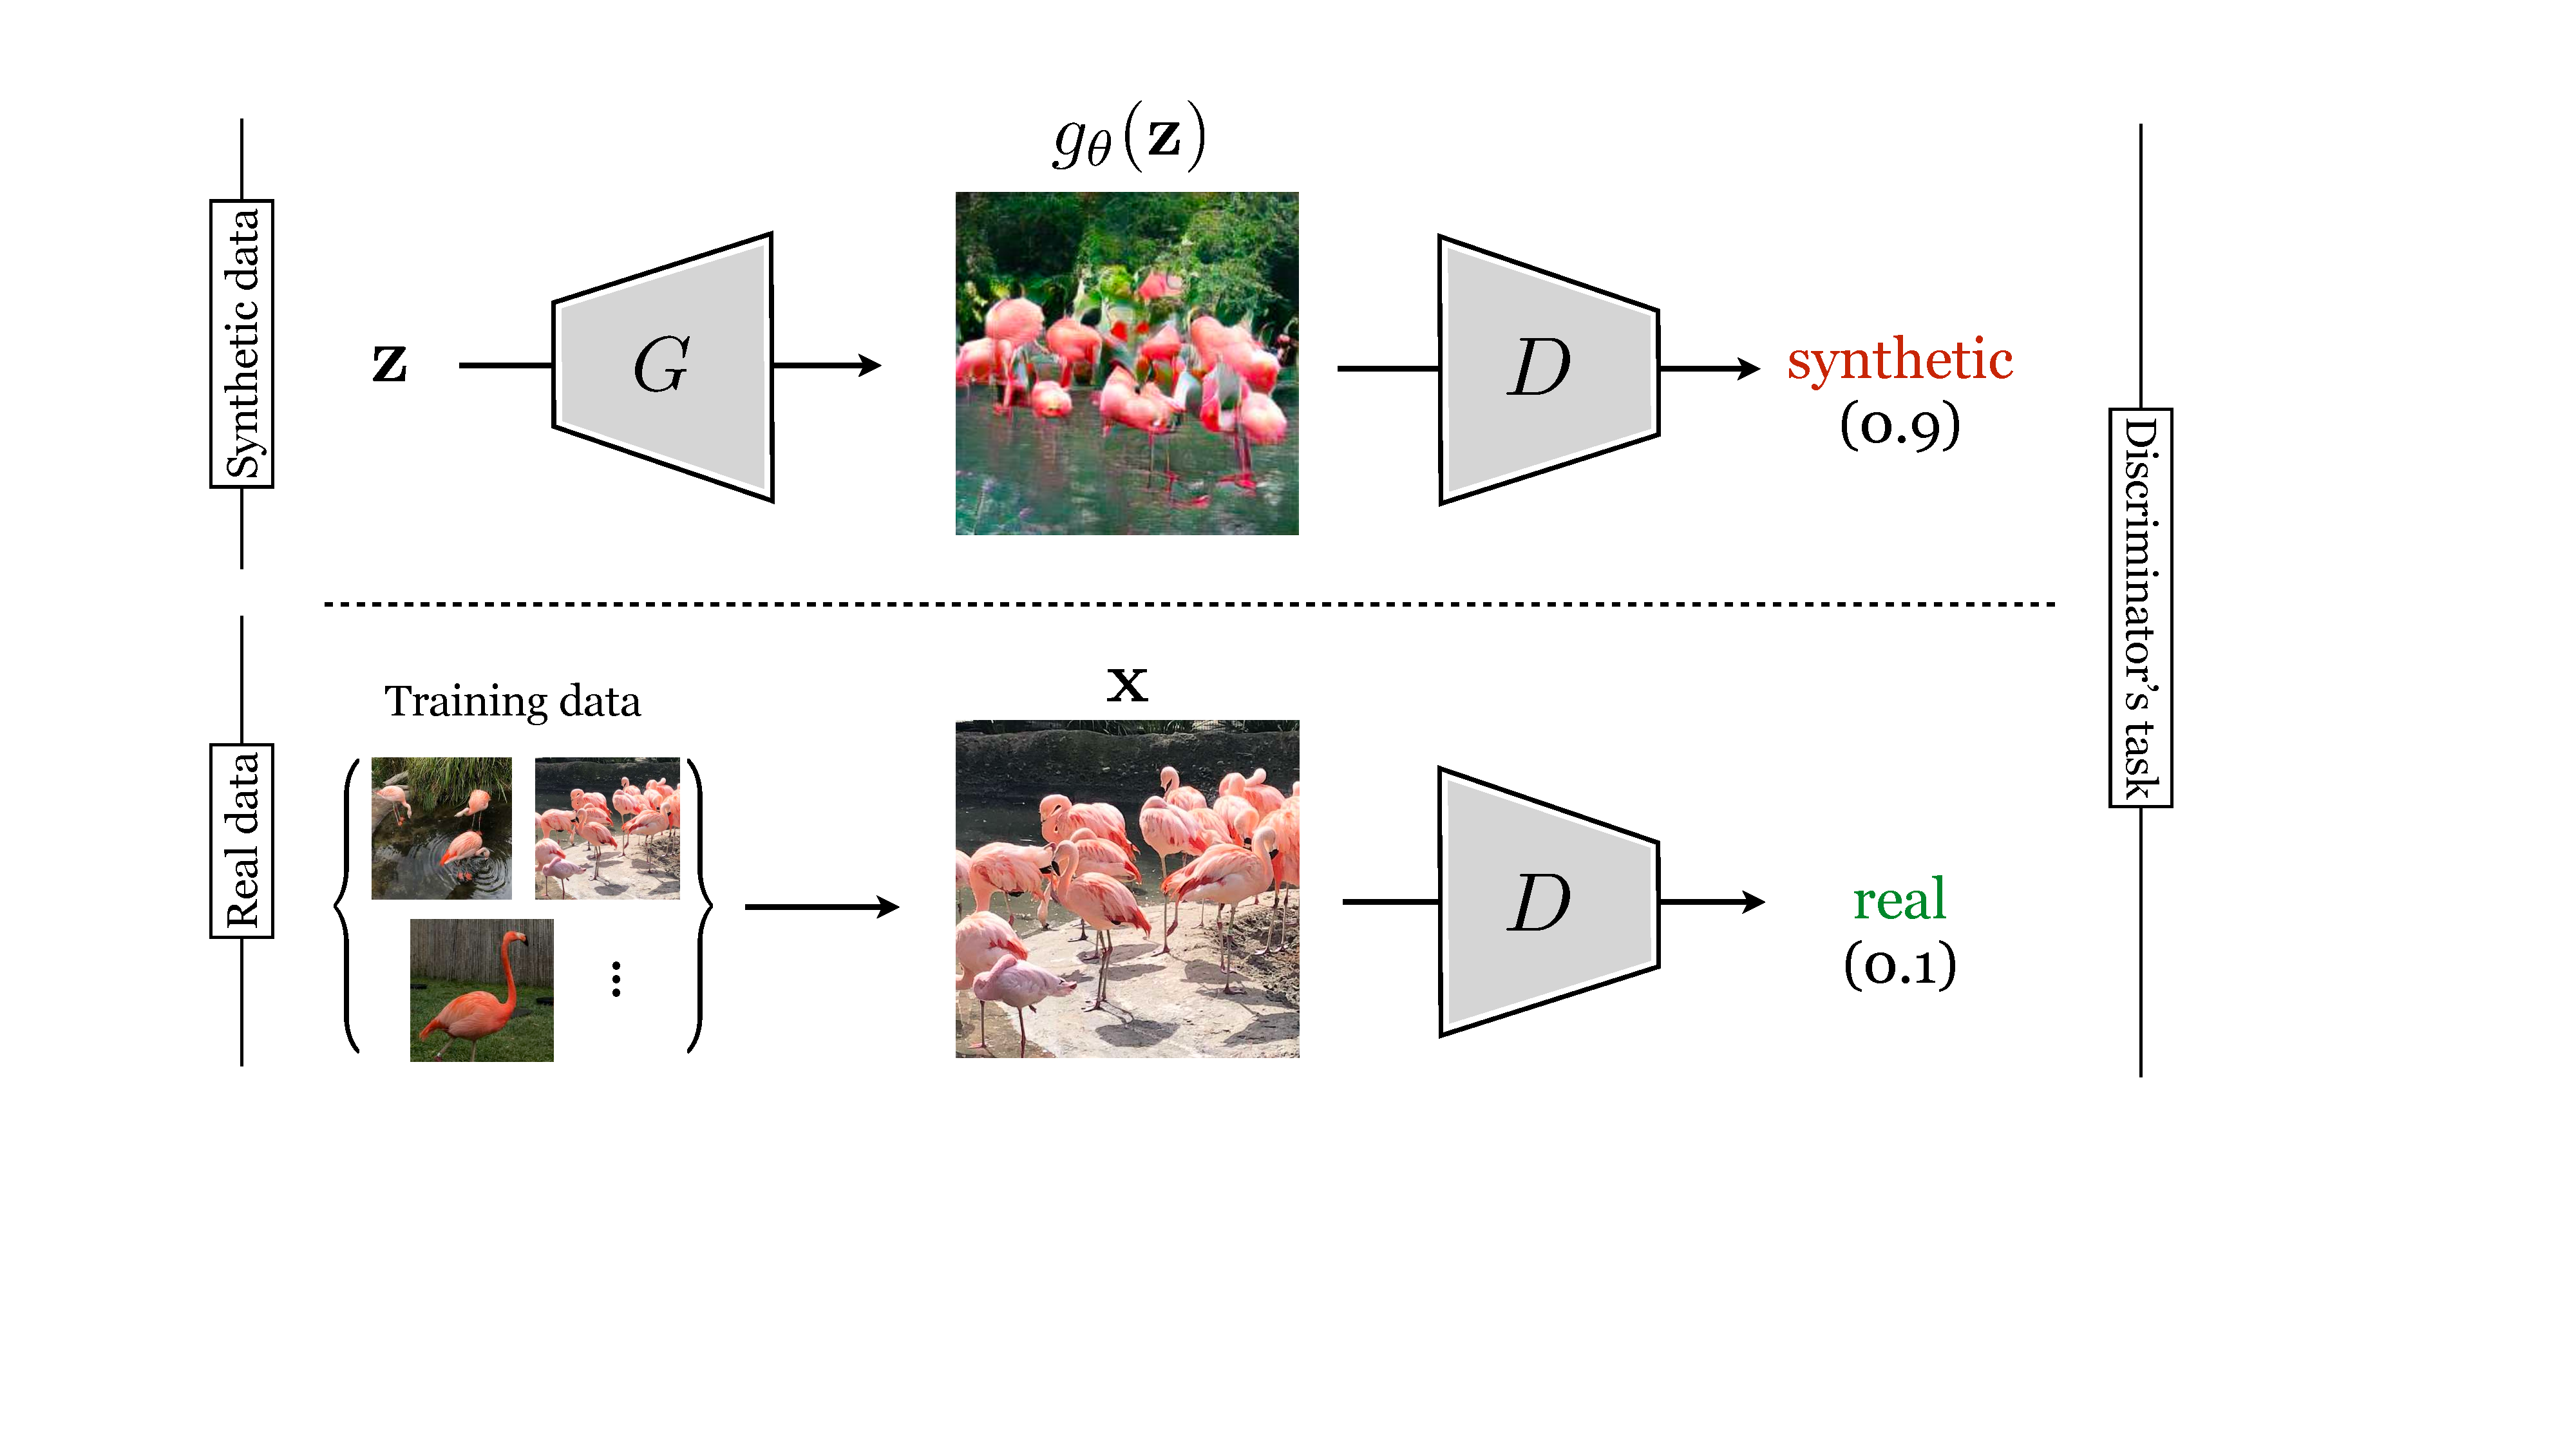
\includegraphics[width=1.0\linewidth]{./figures/generative_models/gan_schematic.pdf}
    }
    \caption{Architecture of a GAN being trained to generate images of flamingos. The synthetic image in this example is generated by BigGAN~\cite{brock2018large}. Notice the artifacts in the synthetic image; after more training, the discriminator could pick up on these and tell the generator to correct them.}
    \label{fig:generative_models:generative_models:gan_schematic}
\end{figure}

Although we call this an adversarial game, the discriminator is in fact helping the generator to perform better and better, by pointing out its current errors (we call it an adversary because it tries to point out errors). You can think of the generator as a student taking a painting class and the discriminator as the teacher. The student is trying to produce new paintings that match the quality and style of the teacher. At first the student paints flat landscapes that lack shading and the illusion of depth; the teacher gives feedback: ``This mountain is not well shaded; it looks 2D.'' So the student improves and corrects the error, adding haze and shadows to the mountain. The teacher is pleased but now points out a different error: ``The trees all look identical; there is not enough variety.'' The teacher and student continue on in this fashion until the student has succeeded at satisfying the teacher. Eventually, in theory, the student—the generator—produces paintings that are just as good as the teacher’s paintings.

This objective may be easier to understand if we think of the objectives for $g_{\theta}$ and $d_{\phi}$ separately. Given a particular generator $g_{\theta}$, $d_{\phi}$ tries to maximize its ability to discriminate between real and synthetic images (synthetic images are anything output by $g_{\theta}$). The objective of $d_{\phi}$ is logistic regression between a set of real data $\{\mathbf{x}^{(i)}\}_{i=1}^N$ and synthetic data $\{\hat{\mathbf{x}}^{(i)}\}_{i=1}^N$, where $\hat{\mathbf{x}}^{(i)} = g_{\theta}(\mathbf{z}^{(i)})$.

Let the optimal discriminator be labeled $d_{\phi}^*$. Then we have, 
\begin{align}
    d_{\phi}^* = \argmax_{\phi} \mathbb{E}_{\mathbf{x} \sim p_{\texttt{data}}}[\log d_{\phi}(\mathbf{x})] + \mathbb{E}_{\mathbf{z} \sim p_{\mathbf{z}}}[\log (1-d_{\phi}(g_{\theta}(\mathbf{z})))] \label{eqn:generative_models:GAN_optimal_D}
\end{align}

Now we turn to $g_{\theta}$'s perspective. Given $d_{\phi}^*$, $g_{\theta}$ tries to solve the following problem:
\begin{align}
    \argmin_{\theta} \mathbb{E}_{\mathbf{z} \sim p_{\mathbf{z}}}[\log (1-d_{\phi}^*(g_{\theta}(\mathbf{z})))] \label{eqn:generative_models:GAN_optimal_G}
\end{align}

Now, because the optimal discriminator $d_{\phi}^*$ depends on the current behavior of $g_{\theta}$, as soon as we \textit{change} $g_{\theta}$, updating it to better fool $d_{\phi}^*$, then $d_{\phi}^*$ no longer is the optimal discriminator and we need to again solve problem in \eqn{\ref{eqn:generative_models:GAN_optimal_D}}. To optimize a GAN, we simply alternate between taking one gradient step on the objective in \eqn{\ref{eqn:generative_models:GAN_optimal_G}} and then $K$ gradient steps on the objective in \eqn{\ref{eqn:generative_models:GAN_optimal_D}}, where the larger the $K$, the closer we are to approximating the true $d_{\theta}^*$. In practice, setting $K=1$ is often sufficient.

%Idea that D is the loss for G. (see AGM script)

%[Show some samples from a GAN during different iterates of training?]

\subsection{GANs are Statistical Image Models}
GANs are related to the image and texture models we saw in \chaps{\ref{chapter:stat_image_models}} and \ref{chap:textures}. For example, in the Heeger-Bergen model (\sect{\ref{section:Heeger_Bergen}}; \cite{RG:Heeger-Bergen95}), we synthesize images with the same statistics as a source texture. This can be phrased as an optimization problem in which we optimize image pixels until certain statistics of the images match those same statistics measured on a source (training) image. In the Heeger-Bergen model the objective is to match subband histograms. In the language of GANs, the loss that checks for such a match is a kind of discriminator; it outputs a score related to the difference between a generated image's statistics and the real image's statistics. However, unlike a GAN, this discriminator is hand-defined in terms of certain statistics of interest rather than learned. Additionally, GANs amortize the optimization via learning. That is, GANs learn a mapping $g_{\theta}$ from latent noise to samples rather than arriving at samples via an optimization process that starts from scratch each time we want to make a new sample.


%\section{Conditional generative models}



% \section{Generative versus Discriminative}
% Classically, a distinction was made between \textbf{discriminative models} and generative models, in the context of data classification problems. The former referred to models of $p(Y \given X)$, where $Y$ represented a \emph{label} and $X$ represented \emph{data}. The latter were models of $p(Y, X)$, which can be factored as $p(X \given Y)p(Y)$ (the idea is that $p(X | Y)$ is a model of how the data is generated). This distinction has become less useful in modern AI, since often it's hard to tell what is a \emph{label} and what is \emph{data} -- generally, both the inputs and outputs to our models are high-dimensional structured objects. %For example, an input may be an image, and an output a label map. Or an input may be a scenegraph and an output may be a photograph.

% These days, generative models usually simply refer to models of $p(X)$ or $p(X \given Y)$ with two key properties: (1) $X$ is high-dimensional (usually we think of it as data); and 2) the dimensions of $X$ are nonindependent.


\section{Concluding Remarks}
Generative models are models that synthesize data. They can be useful for content creation—artistic images, video game assets, and so on—but also are useful for much more. In the next chapters we will see that generative models also learn good \textit{image representations}, and conditional generative models can be viewed as a general framework for answering questions and making predictions. As Richard Feynman famously wrote, ``What I cannot create, I do not understand.''\footnote{https://en.wikiquote.org/wiki/Richard\_Feynman} By modeling creation, generative models also help us understand the visual world around us.


